%\documentclass[handout,xcolor=pdftex,dvipsnames,table,mathserif]{beamer} 
\documentclass[xcolor=pdftex,dvipsnames,table]{beamer}
\usepackage{subfigure}
\usepackage{amsbsy}
\usepackage{tikz}
\usetikzlibrary{arrows}
\usepackage{amsmath,graphicx,dsfont,color}
\usepackage{amsfonts}
\usepackage{amssymb}
\usepackage{array}

\bibliographystyle{apalike}

\setbeamertemplate{bibliography item}{\insertbiblabel}
\setbeamertemplate{bibliography entry title}{}
\setbeamertemplate{bibliography entry location}{}
\setbeamertemplate{bibliography entry note}{}

%Definitiona

\newcommand{\x}{\mathbf{x}}
\newcommand{\X}{\mathbf{X}}
\newcommand{\W}{\mathbf{W}} %Weight
\newcommand{\bais}{\mathbf{b}}%Bais
\newcommand{\act}{\texttt{g}}%Activation
\newcommand{\loss}{L}
\newcommand{\pdata}{\hat{p}_{\texttt{data}}}
\newcommand{\nsize}{n}
\newcommand{\param}{\boldsymbol{\theta}}
\newcommand{\featmap}{\boldsymbol{\phi}}
\newcommand{\EV}{\mathbb{E}}









\title{Deep Learning for Image Analysis - \\ 
	   Visualization of Neural Networks}
\author{Thomas Walter, PhD}
\date{Centre for Computational Biology (CBIO) \\
	  MINES Paris-Tech, PSL Research University \\
	  Institut Curie, PSL Research University \\
	  INSERM U900}


%To include LOGO?
%\logo{\includegraphics[width=.1\columnwidth]{MinesLogo}}
\useinnertheme{rounded}
\usecolortheme{rose}

\usepackage{xcolor}
\definecolor{lightblue}{RGB}{0,200,255}


\setbeamertemplate{footline}[frame number]{}
\setbeamertemplate{navigation symbols}{}
\setbeamertemplate{section in toc}[square]
\setbeamertemplate{items}[square]

%% For image credits on image bottom right
\usepackage[absolute,overlay]{textpos}
\setbeamercolor{framesource}{fg=gray}
\setbeamerfont{framesource}{size=\tiny}
\newcommand{\source}[1]{\begin{textblock*}{4cm}(8.7cm,8.6cm)
    \begin{beamercolorbox}[ht=0.5cm,right]{framesource}
      \usebeamerfont{framesource}\usebeamercolor[fg]{framesource} Credits: {#1}
    \end{beamercolorbox}
\end{textblock*}}


\begin{document}

\begin{frame}
\titlepage
\end{frame}

\begin{frame}{Overview}
\tableofcontents
\end{frame}

%%%%%%%%%%%%%%%%%%%%%%%%%%%%%%%%%%%%%%%%%%%%%%%%%%%%%%%%%%%%%%%%%%%%%%%%%
%%%%%%%%%%%%%%%%%%%%%%%%%%%%%%%%%%%%%%%%%%%%%%%%%%%%%%%%%%%%%%%%%%%%%%%%%
\section{Introduction}

% \subsection{Motivation: visualization and understanding}
\begin{frame}{Motivation: visualization and understanding}
	\begin{itemize}
		\item Convolutional Neural Networks have achieved stunning performance for many tasks, such as image classification, image segmentation and object detection. 
		\item CNN can be difficult to train, and results can be very variable for different settings of hyperparameters. 
		\item It is unclear, how design choices (network architecture, initialization, weight decay, $\ldots$) effect trainability and performance. 
		\item It is not very well understood what Neural Networks actually learn. 
		\item One idea to approach these issues relies on {\bf visualization}.
	\end{itemize}
\end{frame}

\begin{frame}{Motivation: 3 scenarios}
\begin{enumerate}
	\item AI worse than humans: visualization can thus help understanding failure modes to guide the research.
	\item AI on par with humans: establish appropriate trust and identify and remove potential biases. 
	\item AI better than humans: visualization can help in machine teaching.
\end{enumerate}
\end{frame}


% \subsection{Categorization}
% \begin{frame}{Categorization of visualization approaches}
% 	\begin{itemize}
% 		\item Image-dependent visualizations
% 		\item Image-independent visualizations
% 	\end{itemize}
% \end{frame}


%%%%%%%%%%%%%%%%%%%%%%%%%%%%%%%%%%%%%%%%%%%%%%%%%%%%%%%%%%%%%%%%%%%%%%%%%
%%%%%%%%%%%%%%%%%%%%%%%%%%%%%%%%%%%%%%%%%%%%%%%%%%%%%%%%%%%%%%%%%%%%%%%%%
\section{Visualization of filters}
\frame{\frametitle{Overview}\tableofcontents[currentsection]}

\begin{frame}{Filters in Neural Networks}
\begin{figure}[htb]
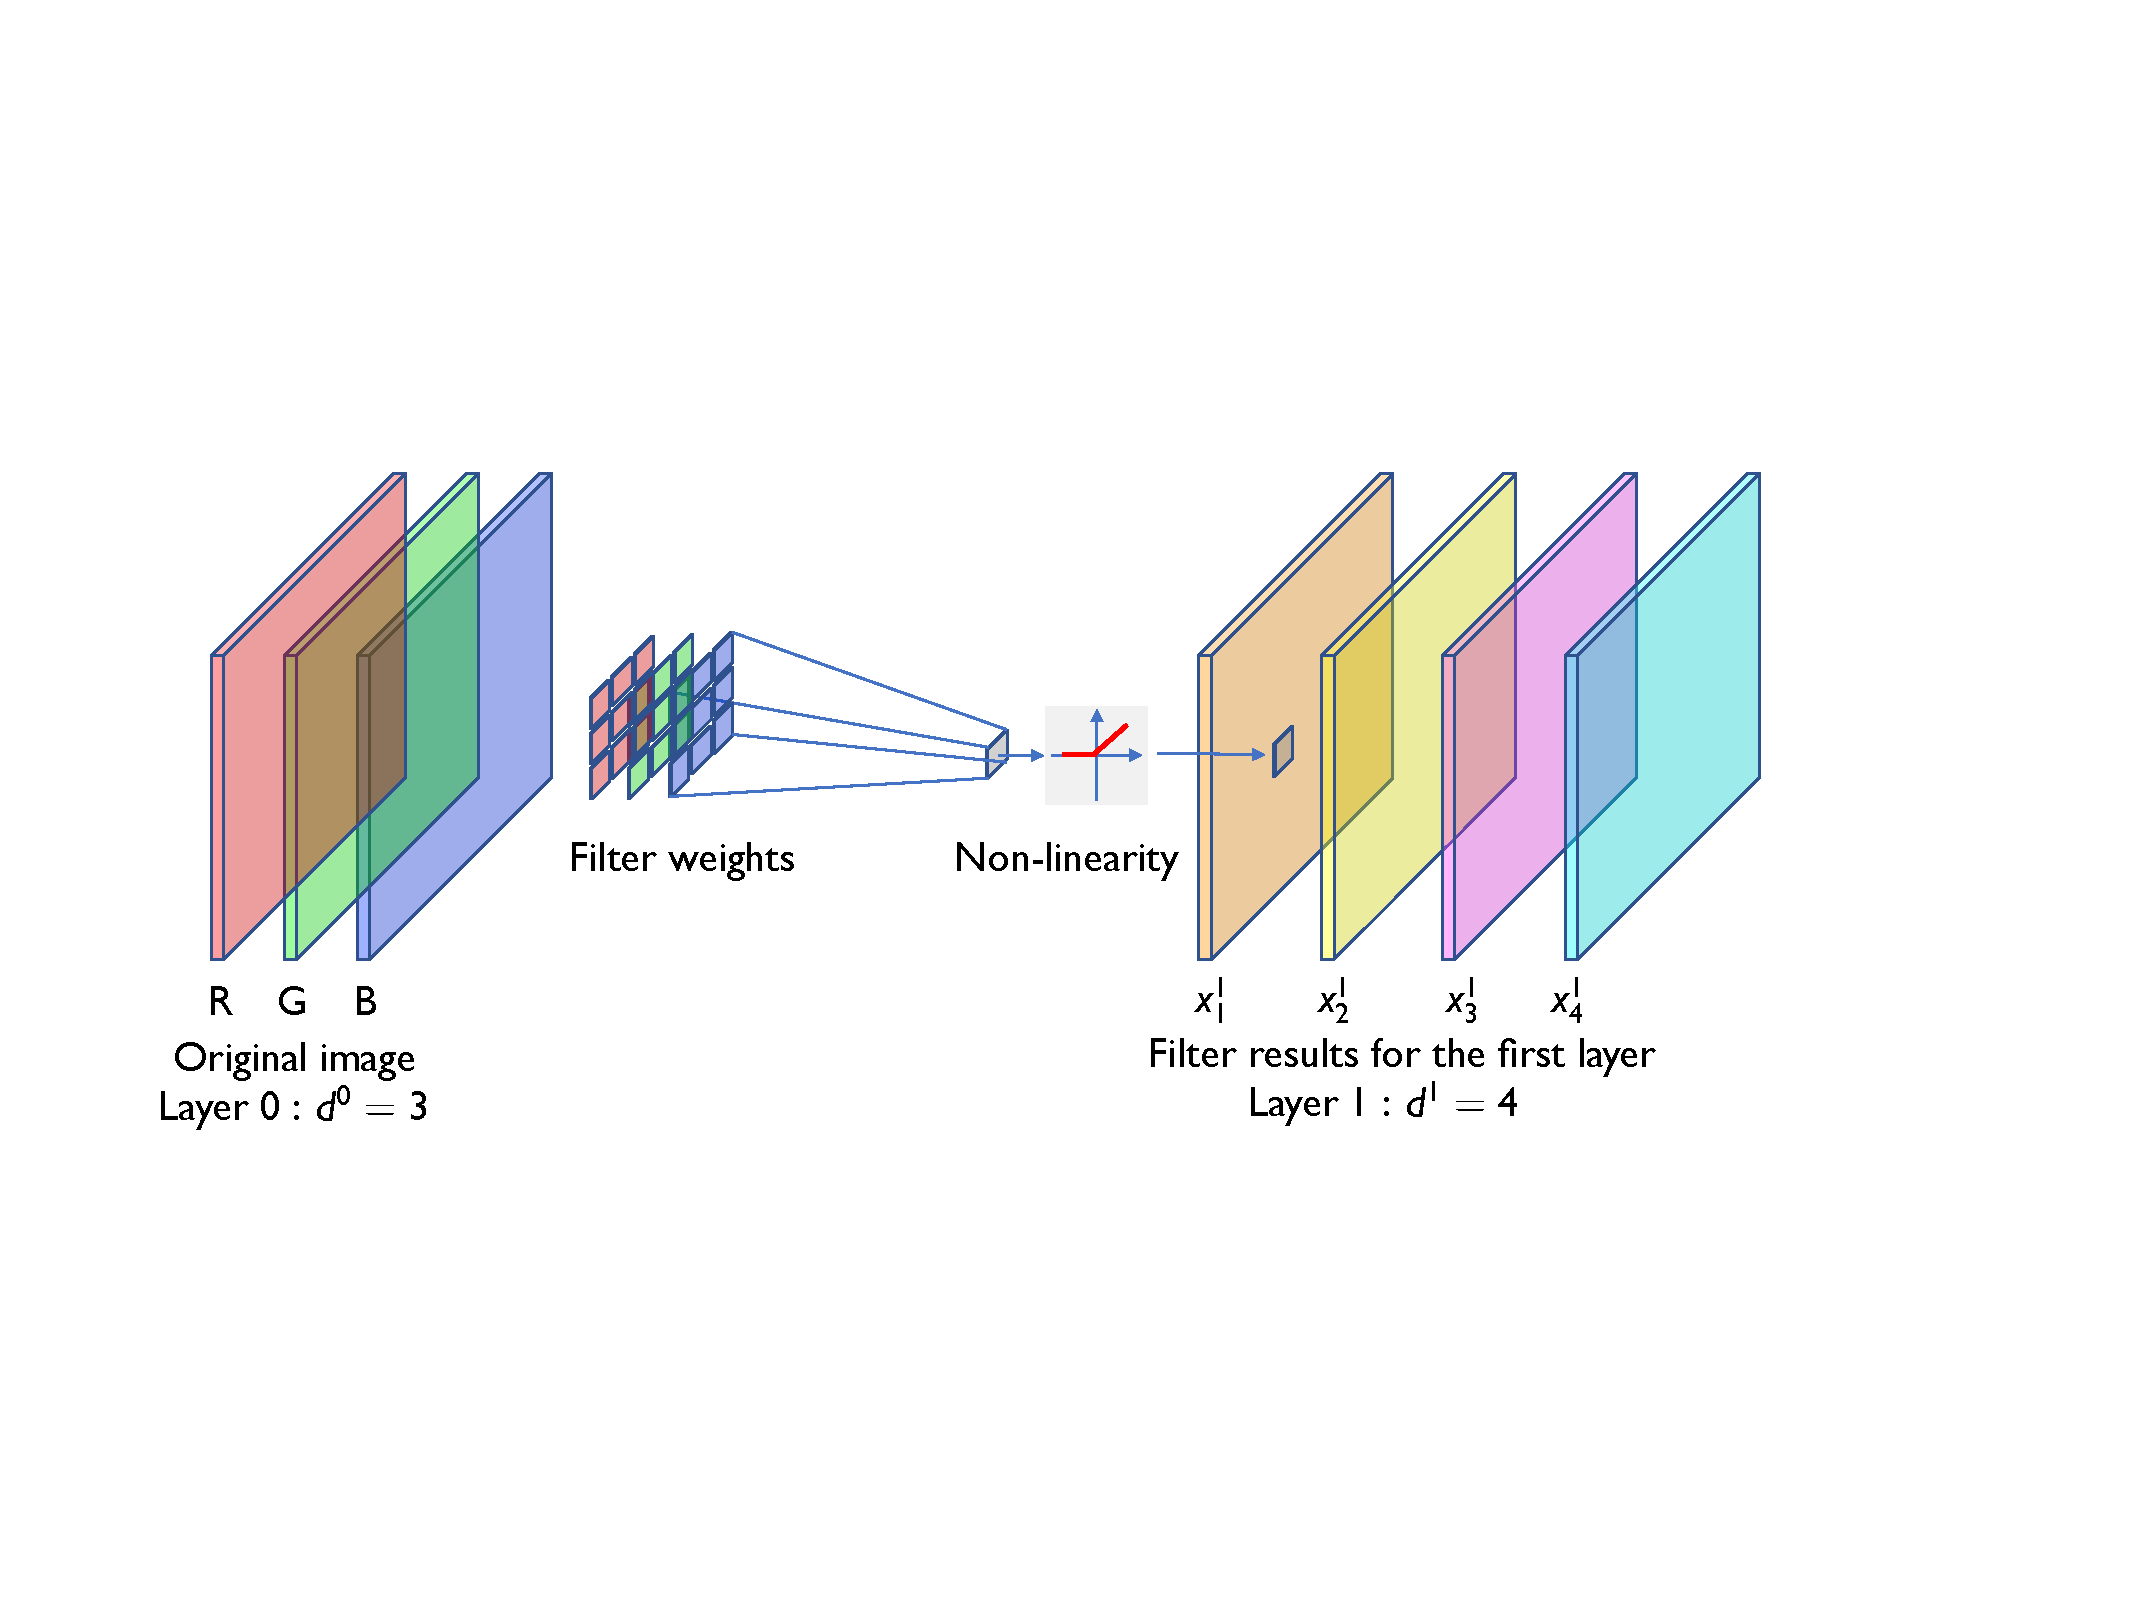
\includegraphics[width=0.9\textwidth]{../graphics/CNN_FirstLayer.pdf}
\end{figure}
In Convolutional Neural Networks (CNN), a pixel value in activation map $r$ in layer $l$ depends on the pixel values in layer $l-1$ within the receptive field of the filter $W^{l}_r$ across all channels. The pixel value $x^{l}_{r}(n,m)$ at position $n,m$ in the activation map $r$ in layer $l$ is\footnote{For simplicity, we do not consider downsampling.}: 
\begin{equation}
	x^{l}_{r}(n,m) = g(\sum_{k}\sum_{i,j}W^{l}_r(i,j,k)x^{l-1}_{k}(n+i,m+j) + b^l_r)
\end{equation} 
\end{frame}

\begin{frame}{Filters in Neural Networks}
\begin{figure}[htb]
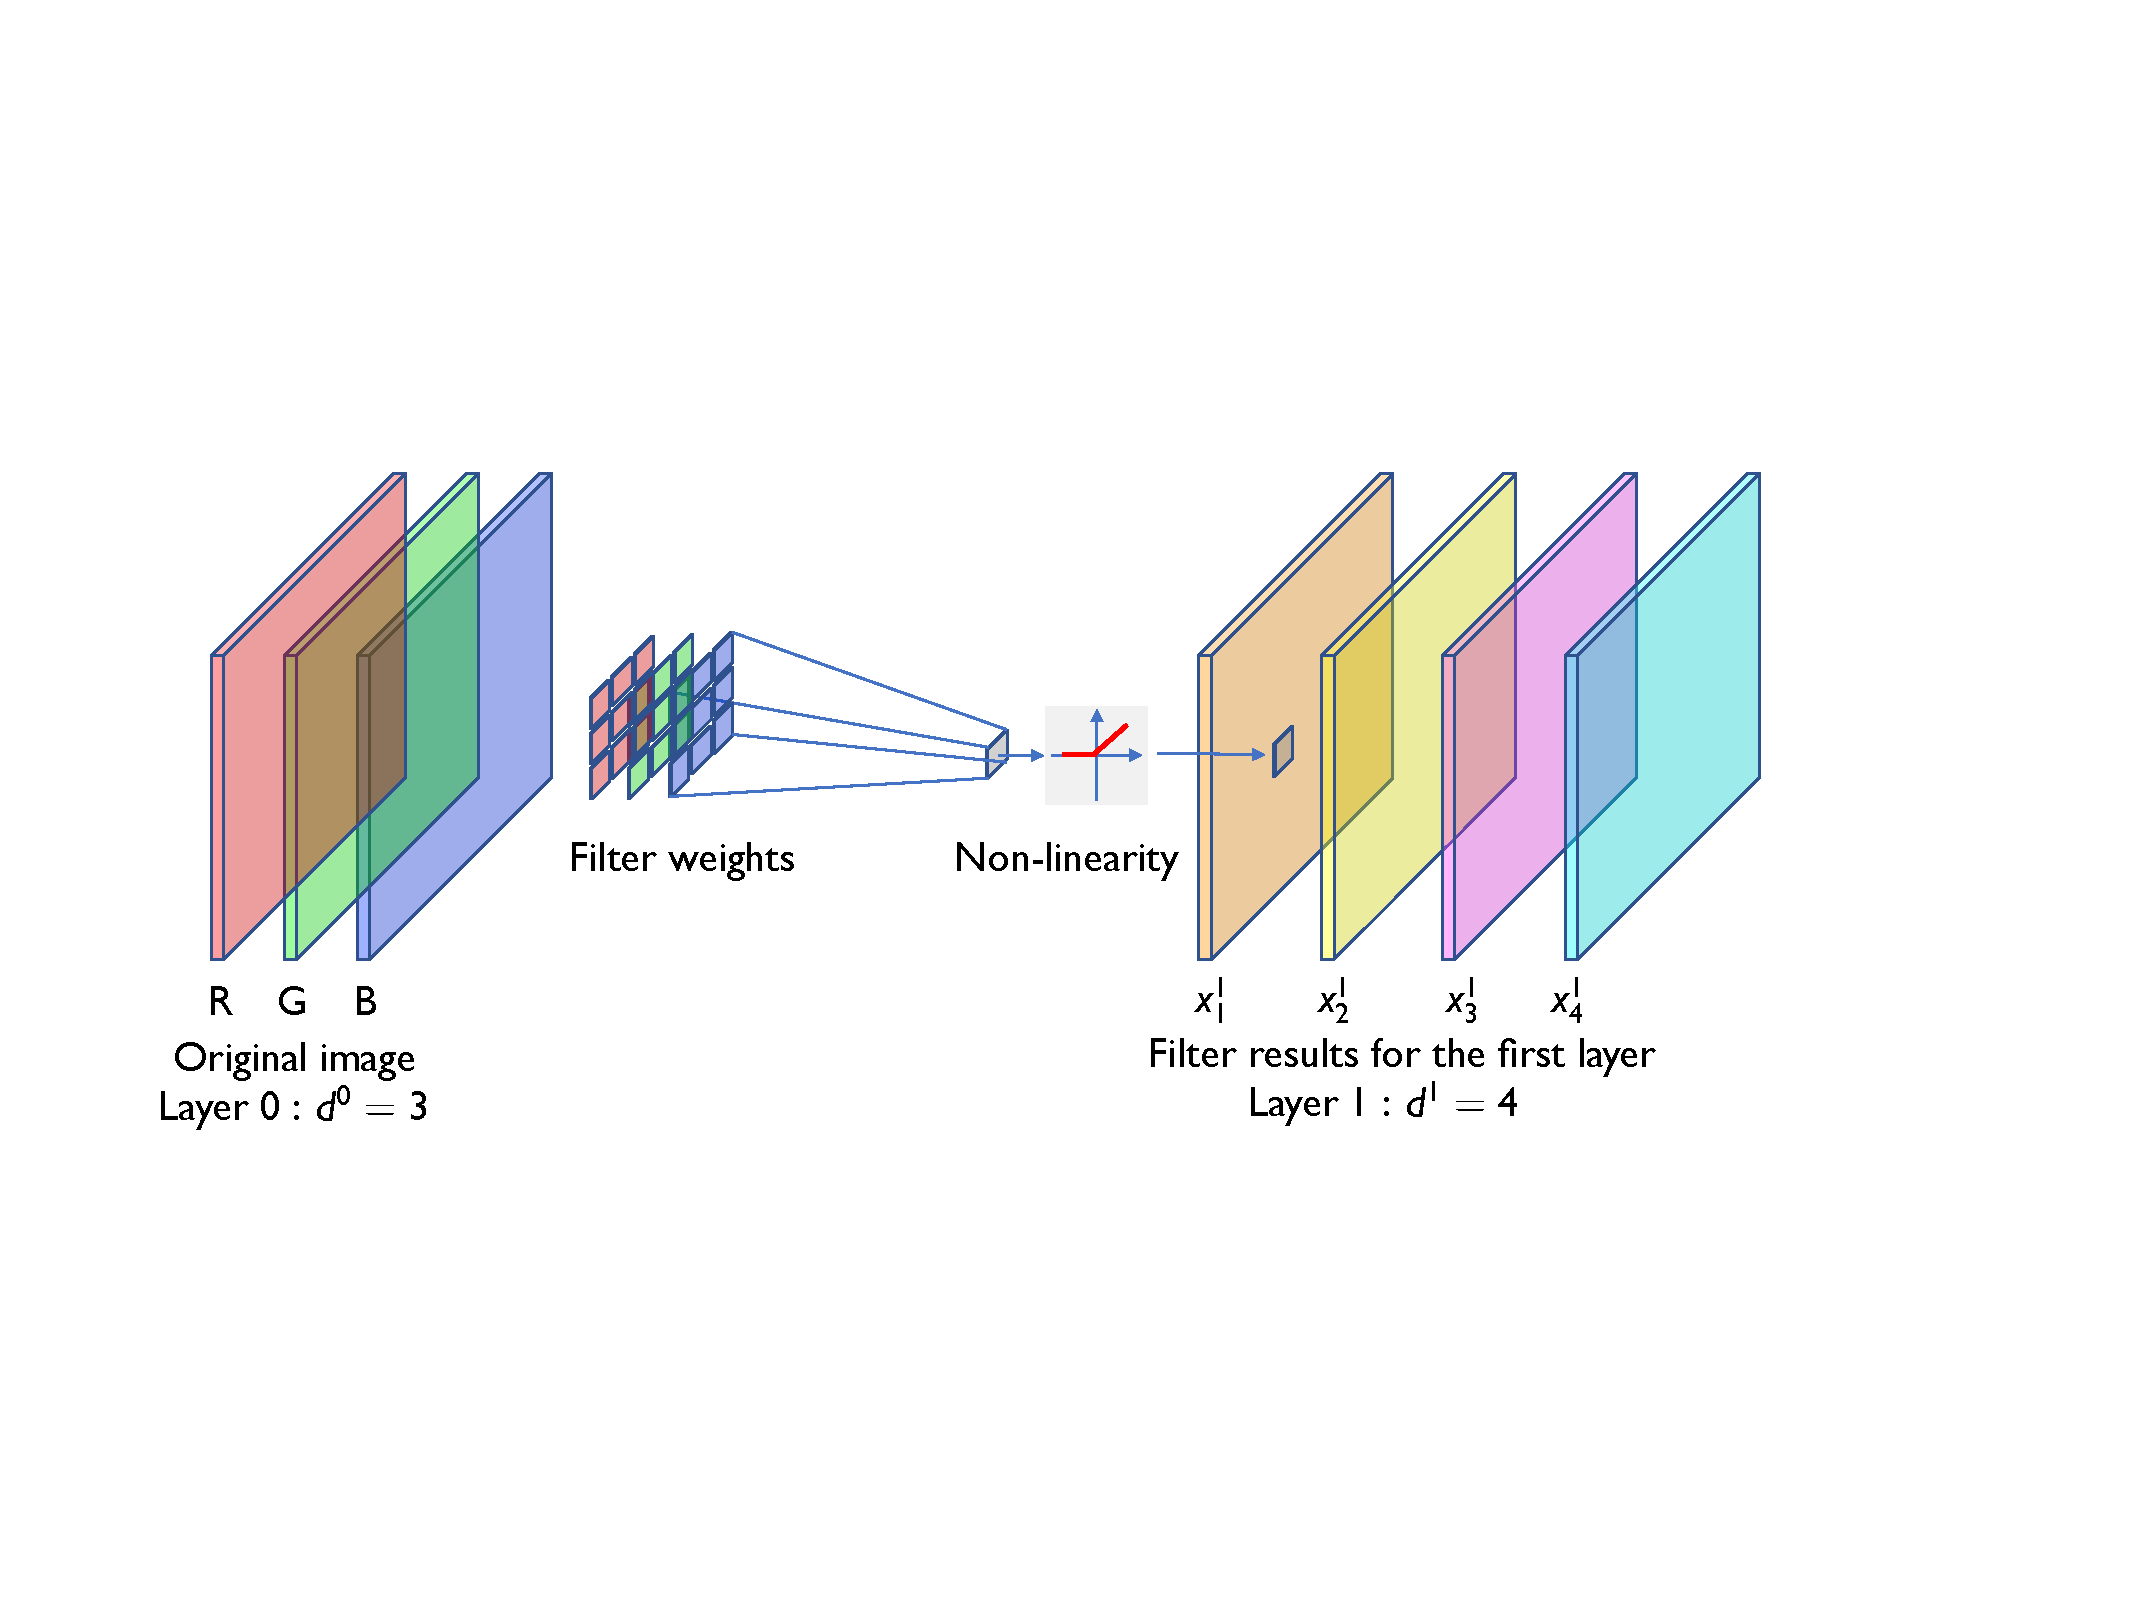
\includegraphics[width=0.9\textwidth]{../graphics/CNN_FirstLayer.pdf}
\end{figure}
\begin{itemize}
	\item Each filter $W^l_r$ (filter $r$ in layer $l$) is thus a 3D tensor of values with dimension $d^{l-1}\times \nu^l\times \nu^l$ ($\nu$: filter width).
	\item For the first layer, the number of input channels is typically 3, i.e. for each pixel, there are 3 values available ($R$, $G$ and $B$).  
	\item For this reason, all filters of layer 1 have the dimension $3\times \nu^{1}\times \nu^{1}$. 
	\item This means that each filter corresponds itself to an $RGB$ image of size $\nu^{1}\times \nu^{1}$. 
\end{itemize}
\end{frame}

\begin{frame}{Visualization of the first layer filters}
\begin{figure}[htb]
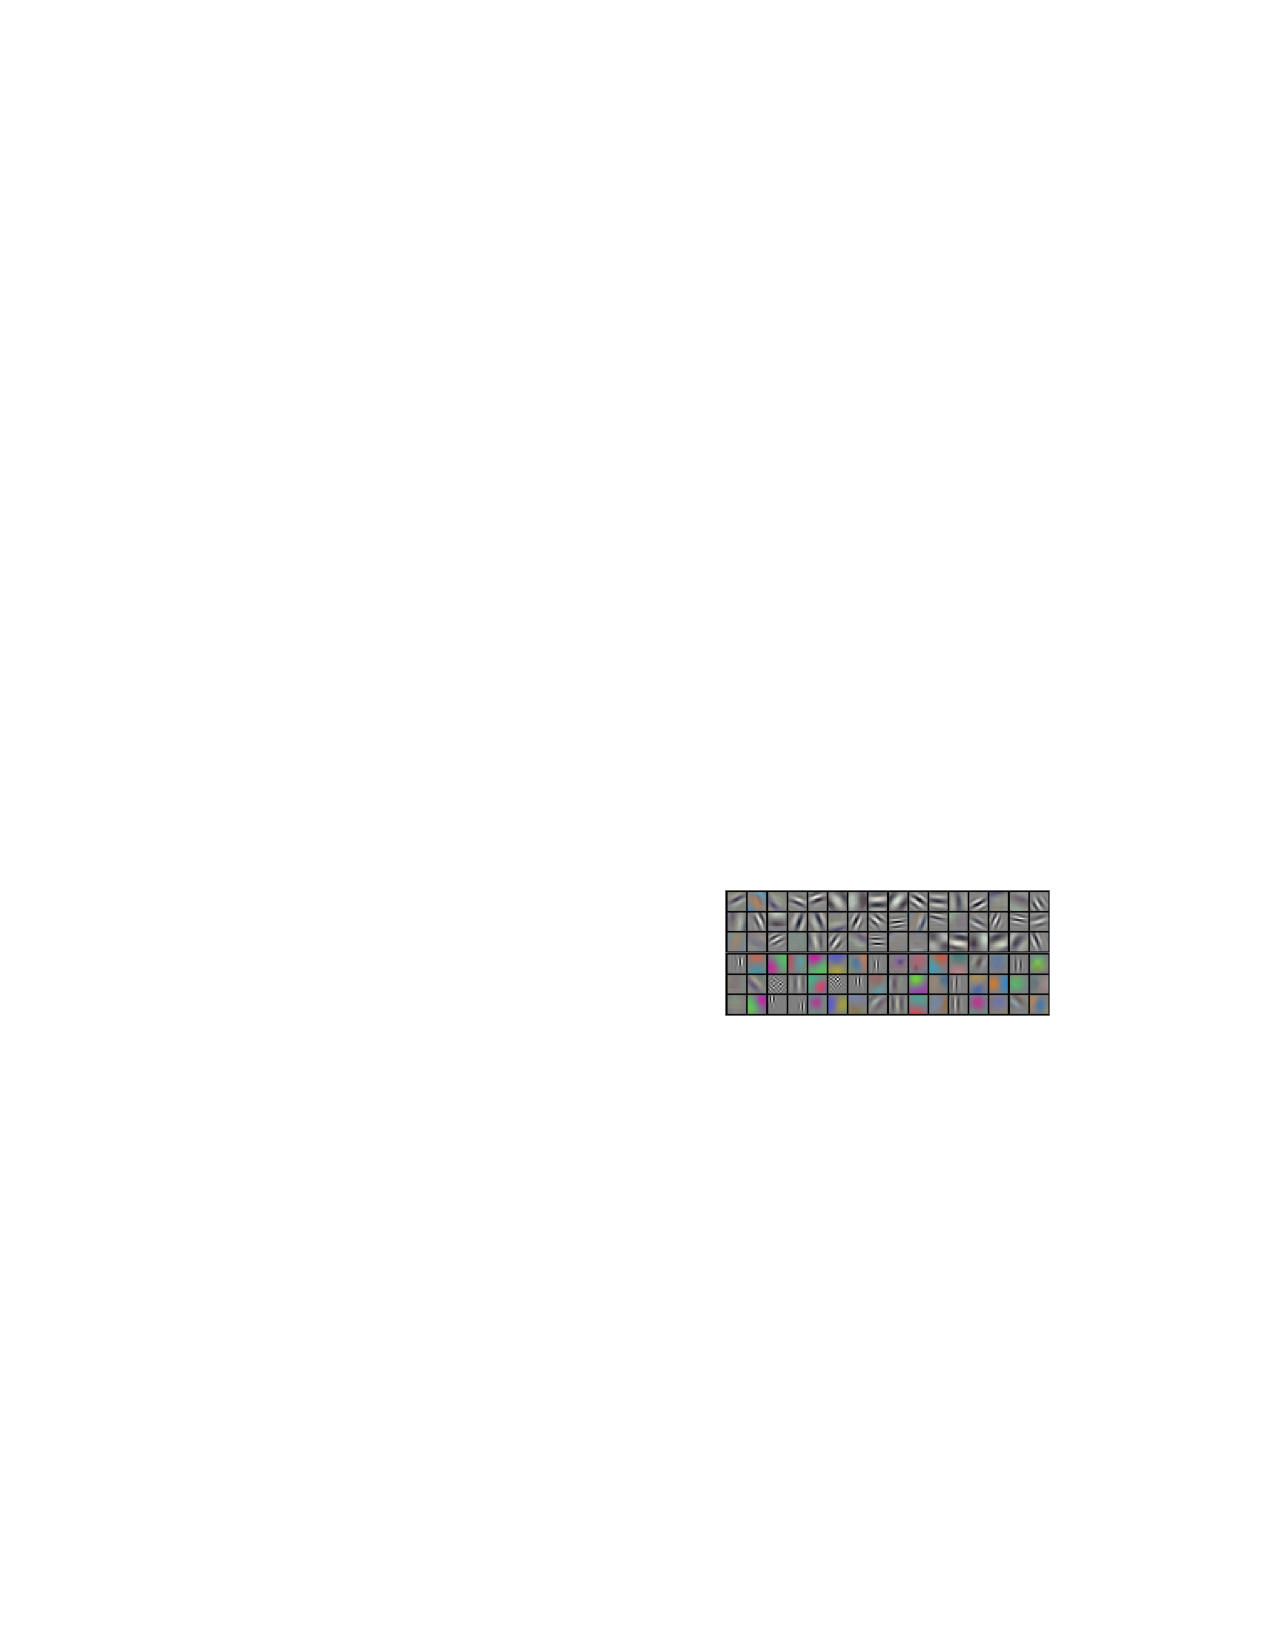
\includegraphics[width=0.9\textwidth]{../graphics/Vis_filter_imagenet.pdf}
\end{figure}
\begin{itemize}
	\item First layer filters obtained by the Alexnet in the Imagenet competition \cite{Krizhevsky:2012}. 
	\item Observation: they contain oriented contours (top row) and color blobs (bottom row). 
	\item How can we interpret this? 
\end{itemize}
\end{frame}

\begin{frame}{Visualization of first layer filters}
\begin{itemize}
	\item The scalar product $w^Tx$ is maximal if $x$ points into the same direction as $w$:
	\begin{equation*}
	w^Tx = \|w\|\|x\|\cos{\alpha_{x,w}}
	\end{equation*}
	\item Consequently the activation maps have high values, if the patterns in the image coincide with the filters. 
	\item We therefore see, that the first layer of a trained convolutional neural network extracts low-level visual information, such as corners, edges, colors. 
	\item The filter visualization strategy is not really applicable to deeper layers: as the filters in deeper layers act on the outputs of the activation maps of the previous filters, it is unclear how to interpret the patterns they might show.
\end{itemize}
\end{frame}

%%%%%%%%%%%%%%%%%%%%%%%%%%%%%%%%%%%%%%%%%%%%%%%%%%%%%%%%%%%%%%%%%%%%%%%%%
%%%%%%%%%%%%%%%%%%%%%%%%%%%%%%%%%%%%%%%%%%%%%%%%%%%%%%%%%%%%%%%%%%%%%%%%%
\section{Visualization of image representations}
\frame{\frametitle{Overview}\tableofcontents[currentsection]}

\begin{frame}{Visualization of image representation}
\begin{figure}[htb]
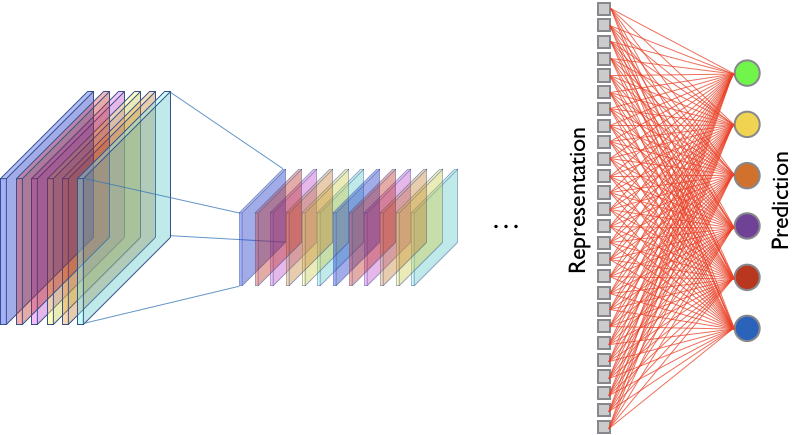
\includegraphics[width=0.8\textwidth]{../graphics/Vis_last_layer.png}
\end{figure}
\begin{itemize}
	\item CNNs learn representations of the images (last layer prior to classification).  
	\item We can now collect these representations $x^{l_{max}}$ for all images in the training set. 
	\item In order to visualize these representations, we seek low dimensional representations of these high dimensional vectors. 
\end{itemize}
\end{frame}

\begin{frame}{t-SNE (sketch) 1/3}
\begin{itemize}
	\item Many low dimensional representations: PCA, ICA, $\ldots$
	\item A recent technique that is widely used in this field is called \emph{t-Distributed Stochastic Neighbor Embedding (t-SNE)} \cite{Maaten:2008}. 
	\item Let $\{x_i\}_{0\leq i < N}$ be the set of representations for all images in the training set. 
	\item We define the pairwise probability that $x_j$ is a neighbor of $x_i$ under the assumption that the neighbor probability is a Gaussian centered in $x_i$:  
	\begin{equation}
	p_{j|i} = \frac{\exp{\left(-\frac{\|x_i - x_j\|^2}{2 \sigma_i^2}\right)}}{\sum_{k\neq i} \exp{\left(-\frac{\|x_i - x_k\|^2}{2 \sigma_i^2}\right)} }
	\end{equation}
	Here, the parameter $\sigma_i$ varies with the sample $x_i$. 
\end{itemize}
\end{frame}


\begin{frame}{t-SNE (sketch) 2/3}
\begin{itemize}

	\item We now want to map the data $\mathcal{X} = \{x_i\}$ to low dimensional representations $\mathcal{Y} = \{y_i\}$ for which these neighborhood probabilities in the projected space $q_{j|i}$ are conserved: 
	\begin{equation}
	q_{j|i} = \frac{\exp{\left(-\|y_i - y_j\|^2\right)}}{\sum_{k\neq i} \exp{\left(-\|y_i - y_k\|^2\right)} }
	\end{equation}
	\item This is achieved by minimizing the Kulback-Leibler divergence between the distributions $P_i$ (distribution of $p_{j|i}$) and $Q_i$ (distribution of $q_{j|i}$): 
	\begin{equation}
		C = \sum_i KL(P_i\|Q_i) = \sum_i \sum_j p_{j|i}\log{\frac{p_{j|i}}{q_{j|i}}}
	\end{equation}
	\item If $x_i$ and $x_j$ are close in the original space, the algorithm will try to push $q_{j|i}$ to become close to $p_{j|i}$. 
	\item If $x_i$ and $x_j$ are far in the original space, they may or may not be far in the projected space. 
\end{itemize}
\end{frame}

\begin{frame}{t-SNE (sketch) 3/3}
\begin{itemize}
	\item The parameters $\sigma_i$ are determined by the algorithm. 
	\item They vary according to the neighbor density, such that for each $x_i$ we have roughly the same number of neighbors. 
	\item The user chooses a value for the \textit{perplexity}, which effectively measures the effective number of neighbors. 
	\item The problem now resumes to solving $\min_{y_i} C$ by gradient descent.
	\item Importantly, this method does not provide a transformation: the minimization is carried out w.r.t. $y_i$. If there is a new datapoint, the minimization problem has to be solved again. 
\end{itemize}
\end{frame}

% \begin{frame}{t-SNE map: example (localization patterns inside cells)}
% \begin{figure}[htb]
%   \centering
%   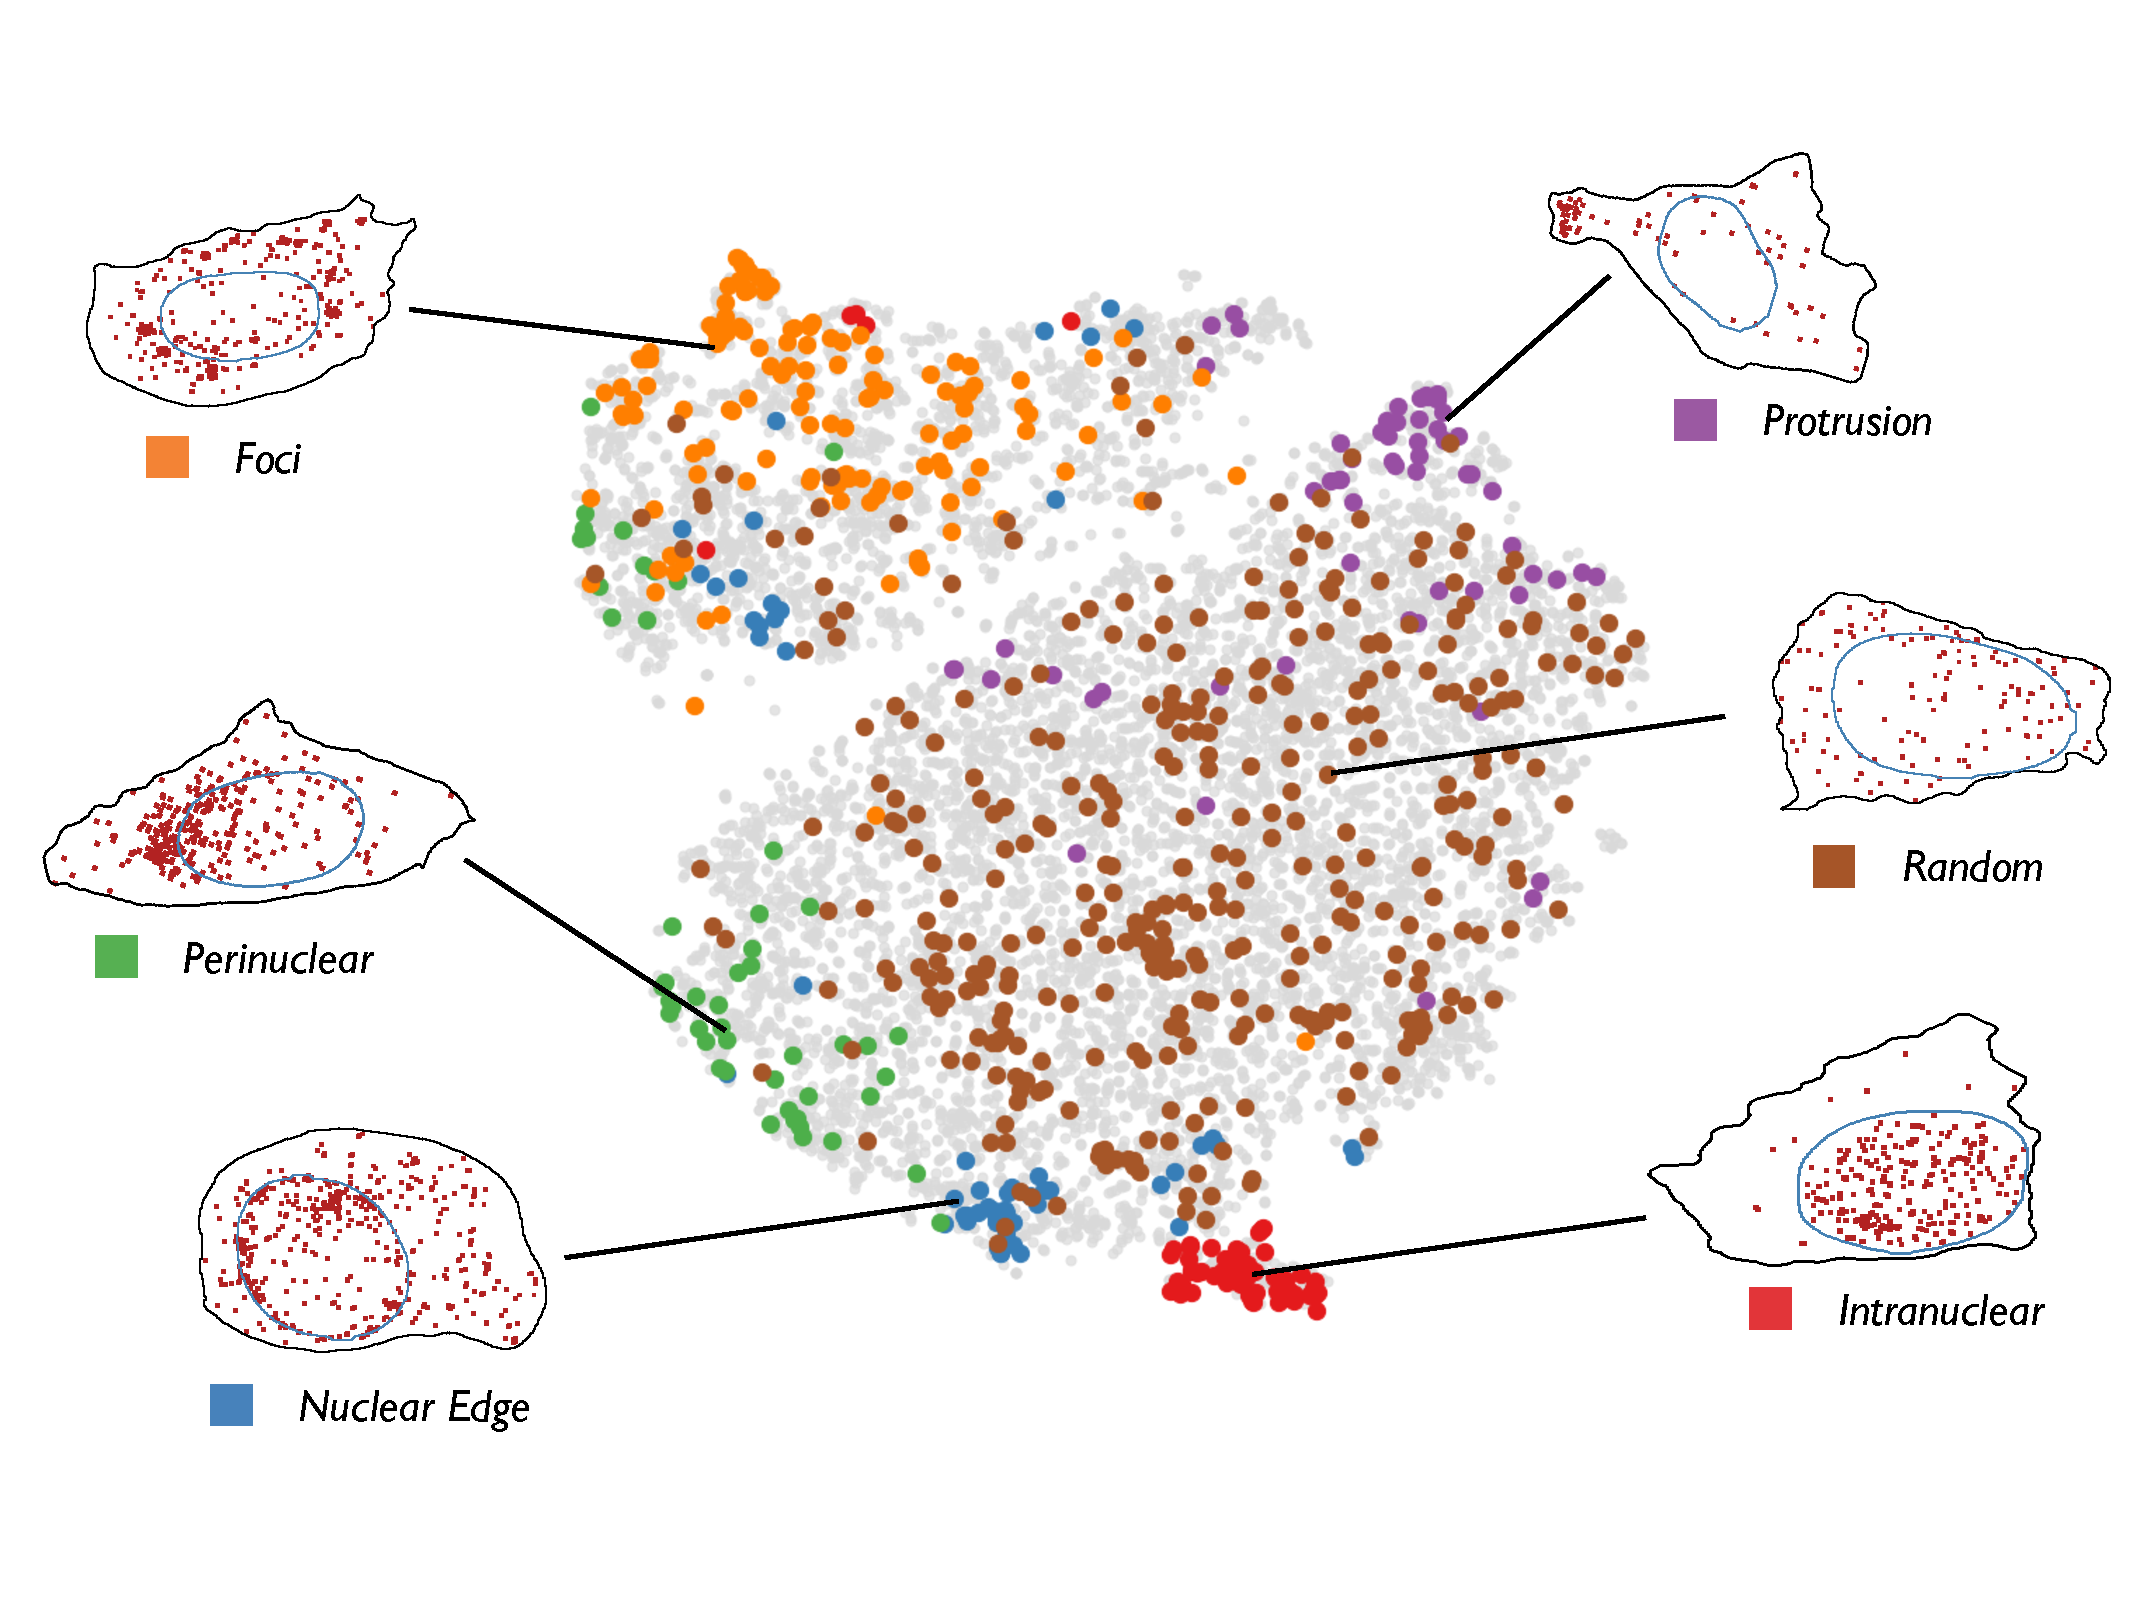
\includegraphics[width=\textwidth]{../graphics/Vis_tsne.pdf}
% \end{figure}
% \end{frame}

\begin{frame}{t-SNE map: ImageNet}
\begin{figure}[htb]
  \centering
  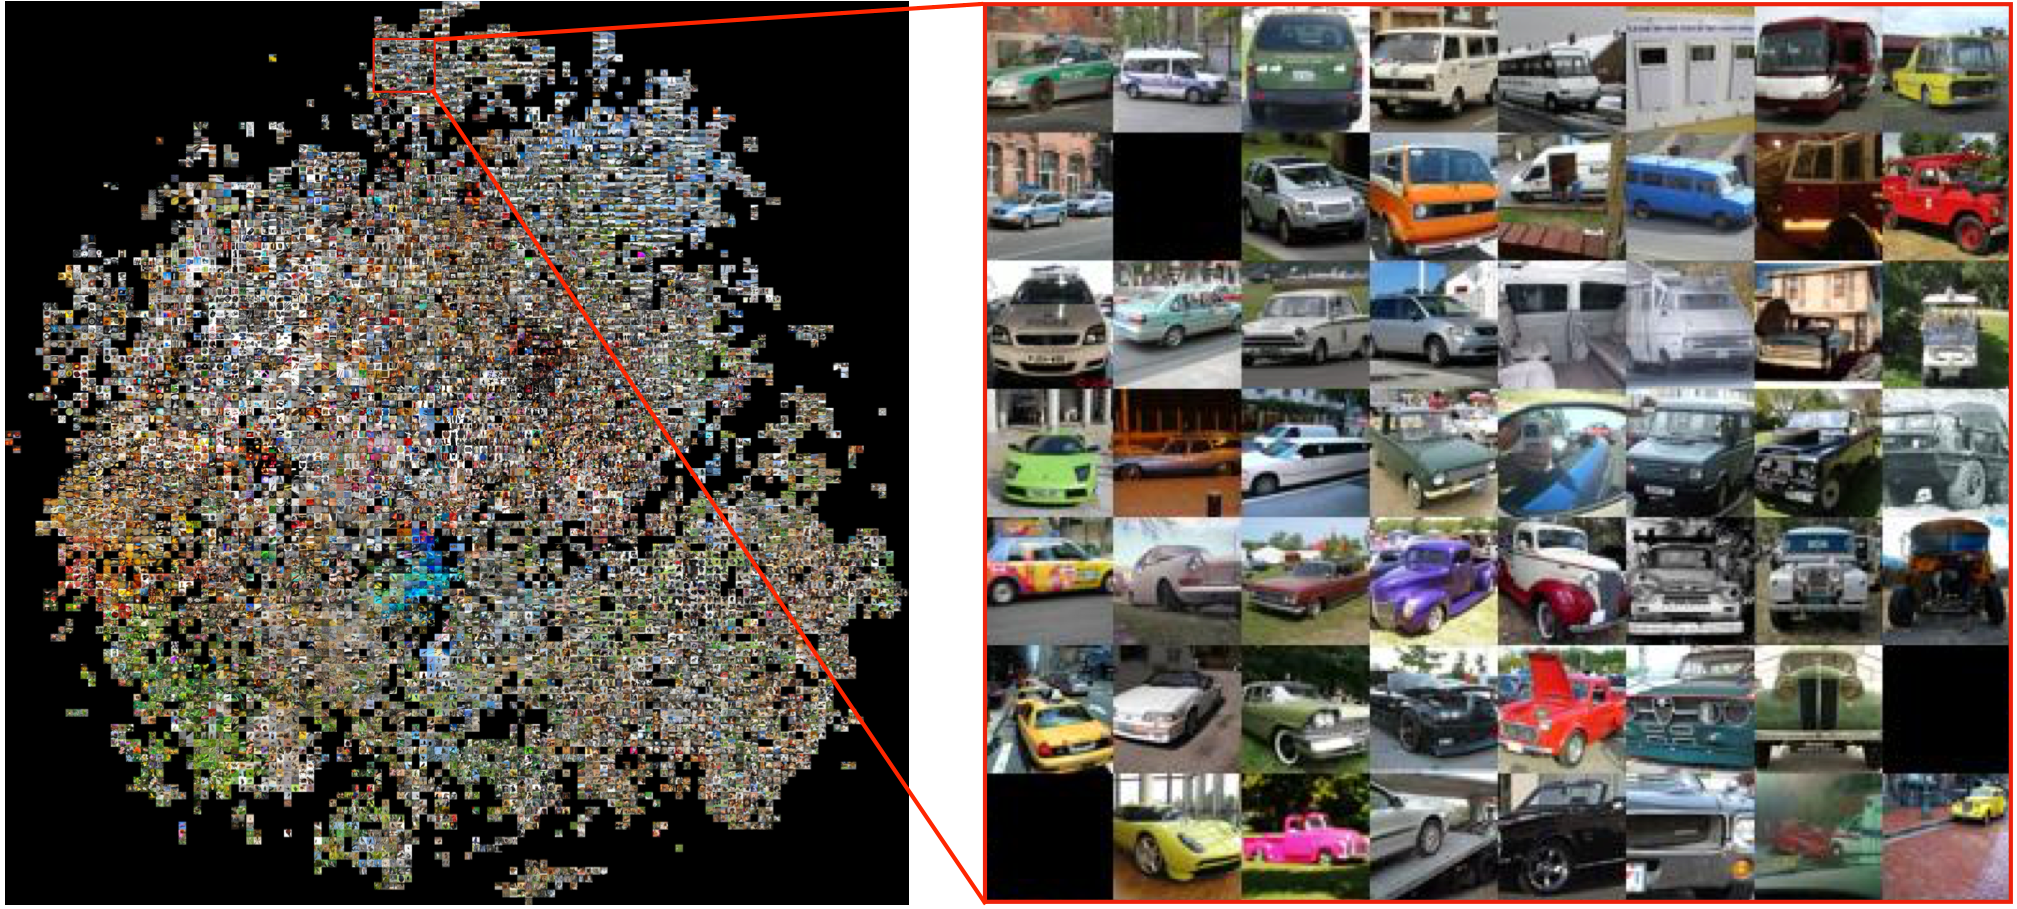
\includegraphics[width=\textwidth]{../graphics/Vis_tsne_imagenet1.pdf}
  \source{adapted from \url{https://cs.stanford.edu/people/karpathy/cnnembed/}}
\end{figure}
\end{frame}

\begin{frame}{t-SNE map: ImageNet}
\begin{figure}[htb]
  \centering
  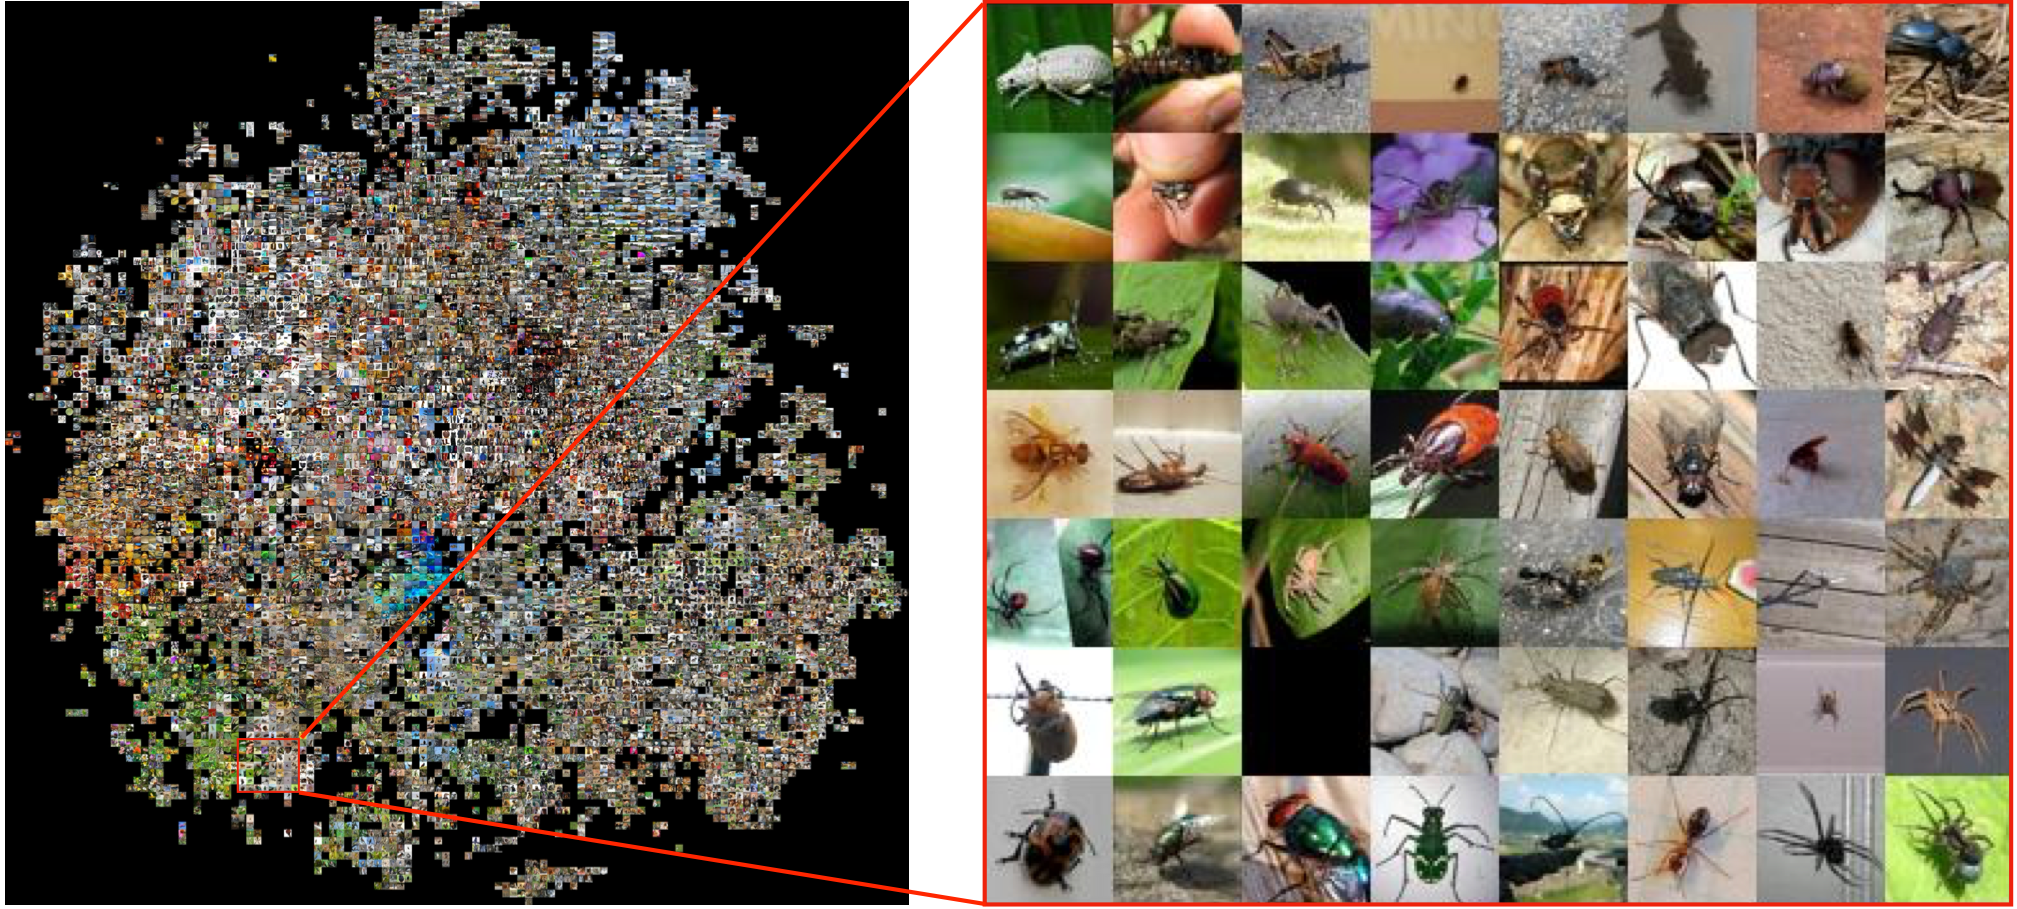
\includegraphics[width=\textwidth]{../graphics/Vis_tsne_imagenet2.pdf}
  \source{adapted from \url{https://cs.stanford.edu/people/karpathy/cnnembed/}}
\end{figure}
\end{frame}

\begin{frame}{t-SNE map: ImageNet}
\begin{figure}[htb]
  \centering
  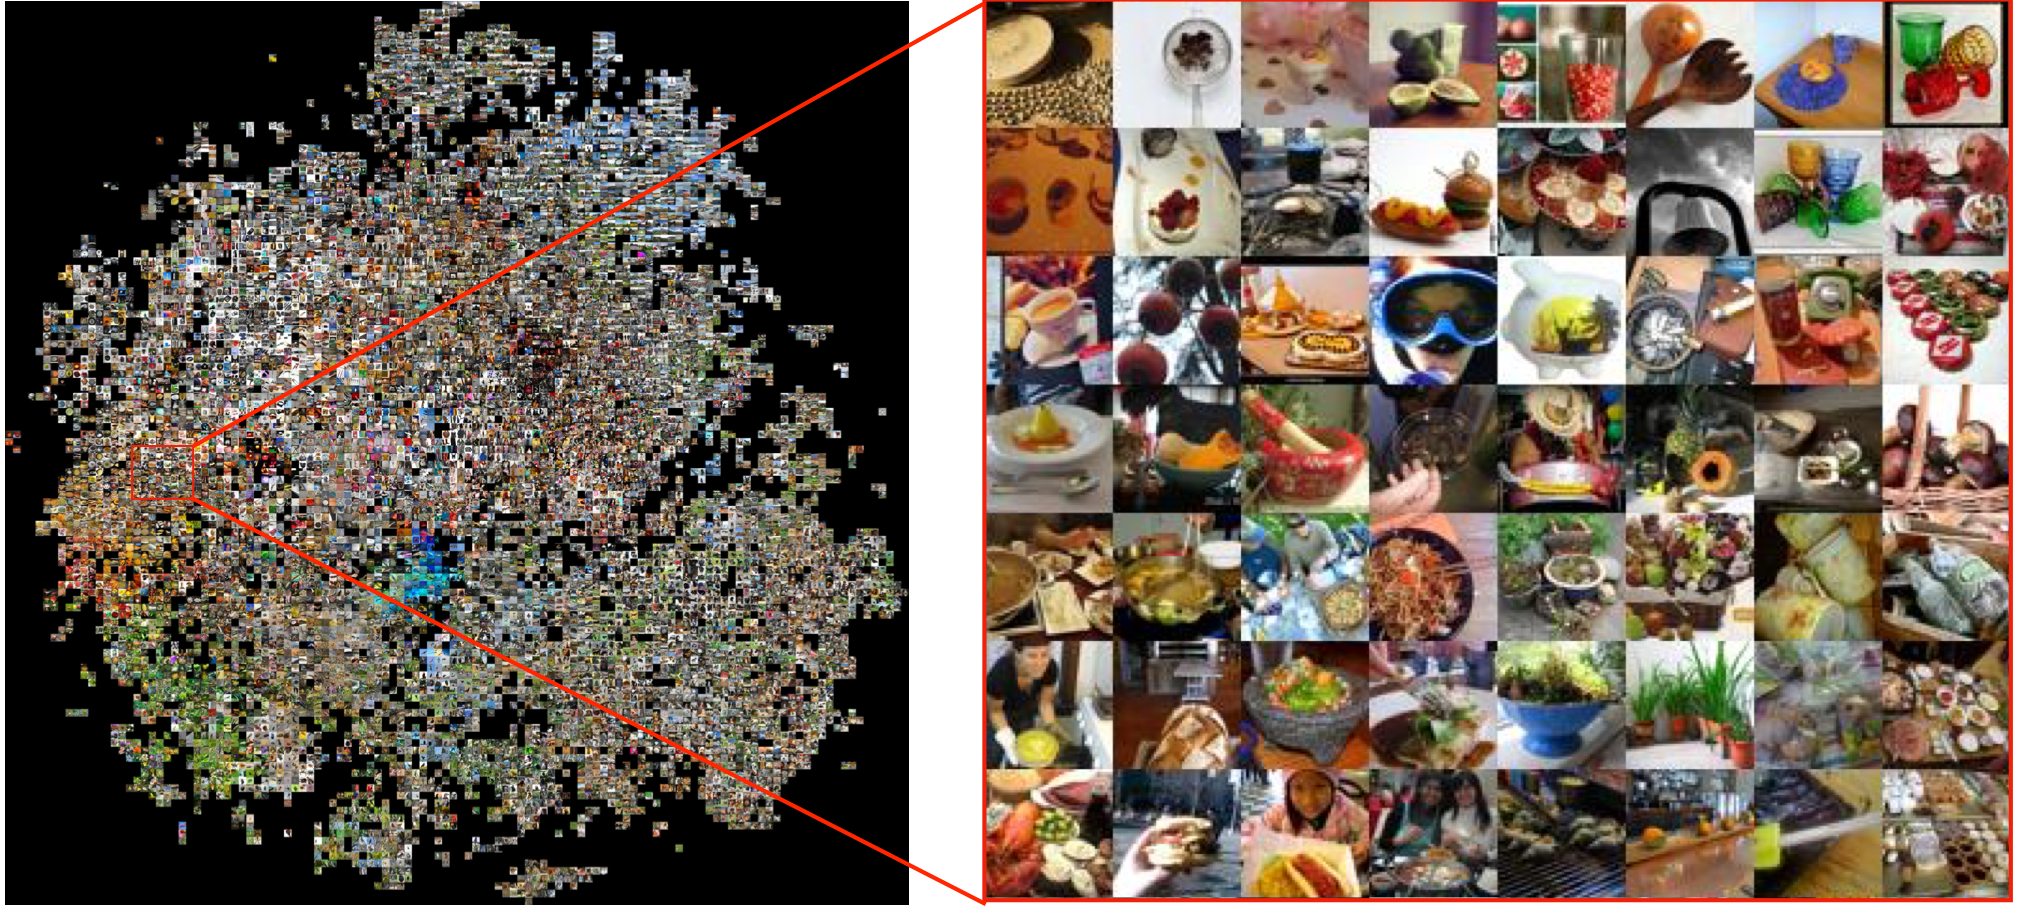
\includegraphics[width=\textwidth]{../graphics/Vis_tsne_imagenet3.pdf}
  \source{adapted from \url{https://cs.stanford.edu/people/karpathy/cnnembed/}}
\end{figure}
\end{frame}

%%%%%%%%%%%%%%%%%%%%%%%%%%%%%%%%%%%%%%%%%%%%%%%%%%%%%%%%%%%%%%%%%%%%%%%%%
%%%%%%%%%%%%%%%%%%%%%%%%%%%%%%%%%%%%%%%%%%%%%%%%%%%%%%%%%%%%%%%%%%%%%%%%%
\section{Visualization of input output relationships}
\frame{\frametitle{Overview}\tableofcontents[currentsection]}

\begin{frame}{Saliency maps}
	\begin{figure}[htb]
	  \centering
	  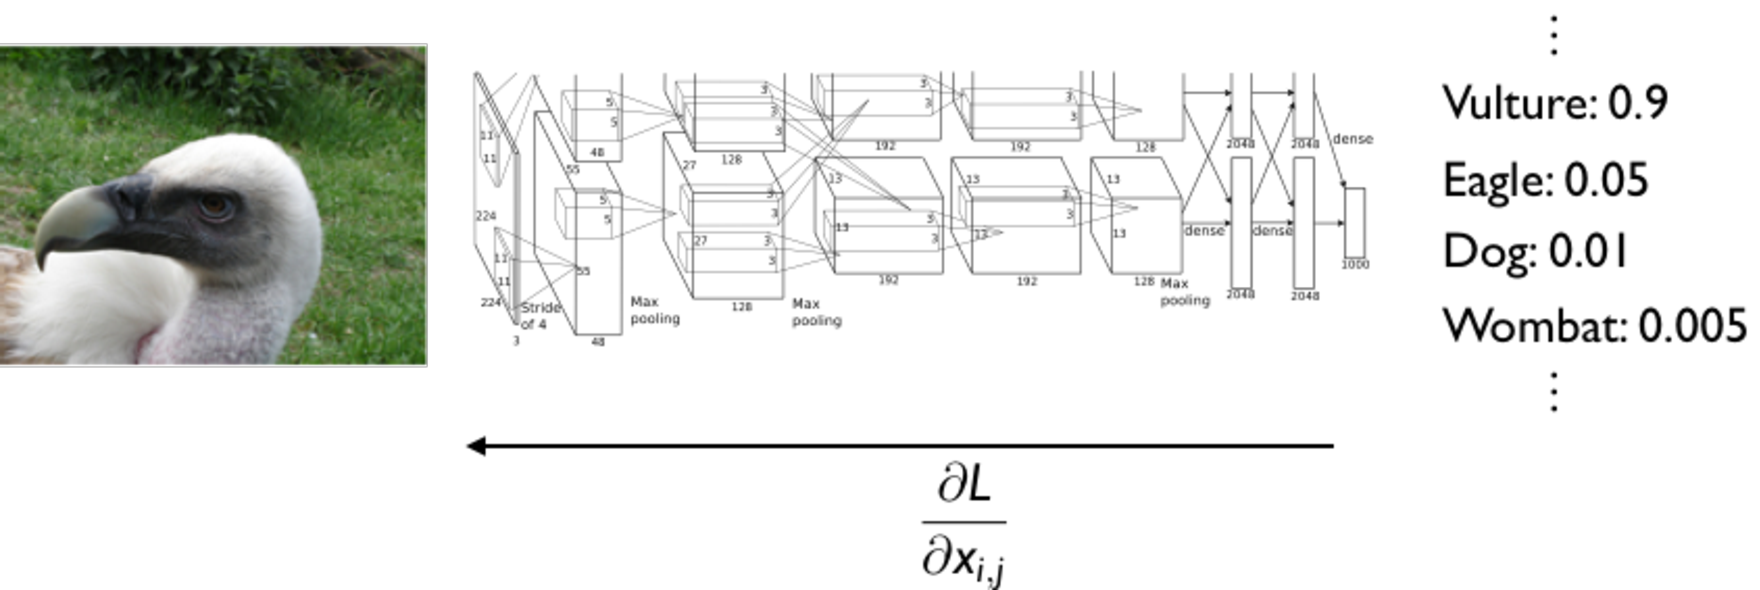
\includegraphics[width=\textwidth]{../graphics/Vis_saliency_map_principle.pdf}
	\end{figure}
\begin{itemize}
	\item For each pixel in the input image we can calculate the derivative of the loss with respect to that pixel value \cite{Simonyan:2013}.
	\item This allows us to visualize how much the loss changes with small variations of the pixel values.
	\item Calculation: simple backgropagation 
\end{itemize}
\end{frame}

% \begin{frame}{Saliency maps}
% \begin{itemize}
% 	\item Calculation: simple backpropagation:
% 	\begin{equation}
% 		\left|\frac{\partial L}{\partial x_{i,j}}\right|
% 	\end{equation} 
% 	\item Unpooling: the gradient is redirected to the selected input neuron (the one with maximal activation).
% 	\item ReLu: multiplication of the backpropagated gradient signal by the indicator function.
% 	\item Filtering: convolution with the transposed filter response.
% 	\begin{eqnarray}
% 		z &=& x \ast W \nonumber \\
% 		\frac{\partial L}{\partial x} &=& \frac{\partial L}{\partial z} \ast W^T 
% 	\end{eqnarray}
% \end{itemize}
% \end{frame}


\begin{frame}{Saliency maps}
\begin{figure}[htb]
  \centering
  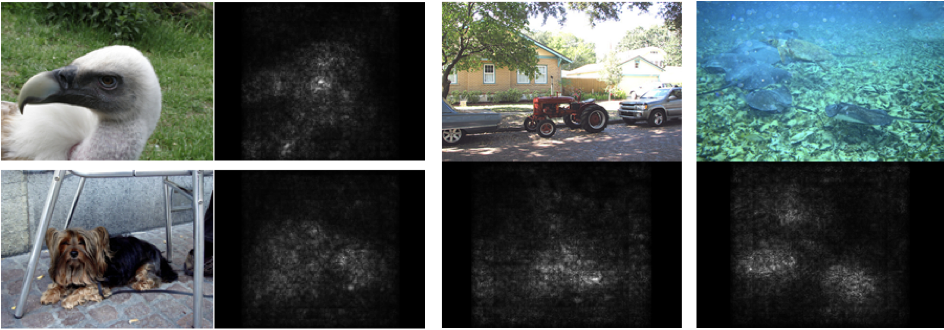
\includegraphics[width=\textwidth]{../graphics/Vis_saliency_maps.png}
  \source{adapted from \cite{Simonyan:2013}}
\end{figure}
Sensitivity analysis: we can see which pixels would have most effect on the classification results. 
\end{frame}

% \begin{frame}{Saliency maps - limitations }
% \begin{itemize}
% 	\item Individual pixels may only marginally contribute to the output. 
% 	\item 
% \end{itemize}
% \end{frame}


\begin{frame}{Occlusion of image patches}
	\begin{itemize}
		\item The output of a classification network is a vector of posterior probabilities $P(y|x)$, where $x$ is the image and $y$ the class label. 
		\item Experiment: we occlude a patch in the image and obtain a changed probability \cite{Zeiler:2013}. 
		\item Now we can assign to every position of the patch in the original image the probability of the correct class and the class label with maximal posterior probability. 
		\item While we can therefore measure the importance of parts of the image with respect to the classification result, this method is slow and not very elegant. 
	\end{itemize}
\end{frame}

\begin{frame}{Occlusion of image patches}
\begin{figure}[htb]
  \centering
  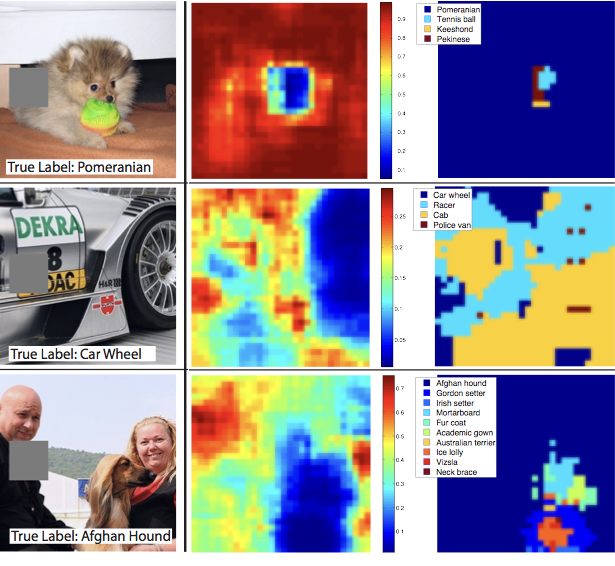
\includegraphics[width=.75\textwidth]{../graphics/Vis_occlusion.png}
  \source{adapted from \cite{Zeiler:2013}}
\end{figure}
\end{frame}

\begin{frame}{Class Activation Mapping (CAM)}
\begin{figure}[htb]
  \centering
  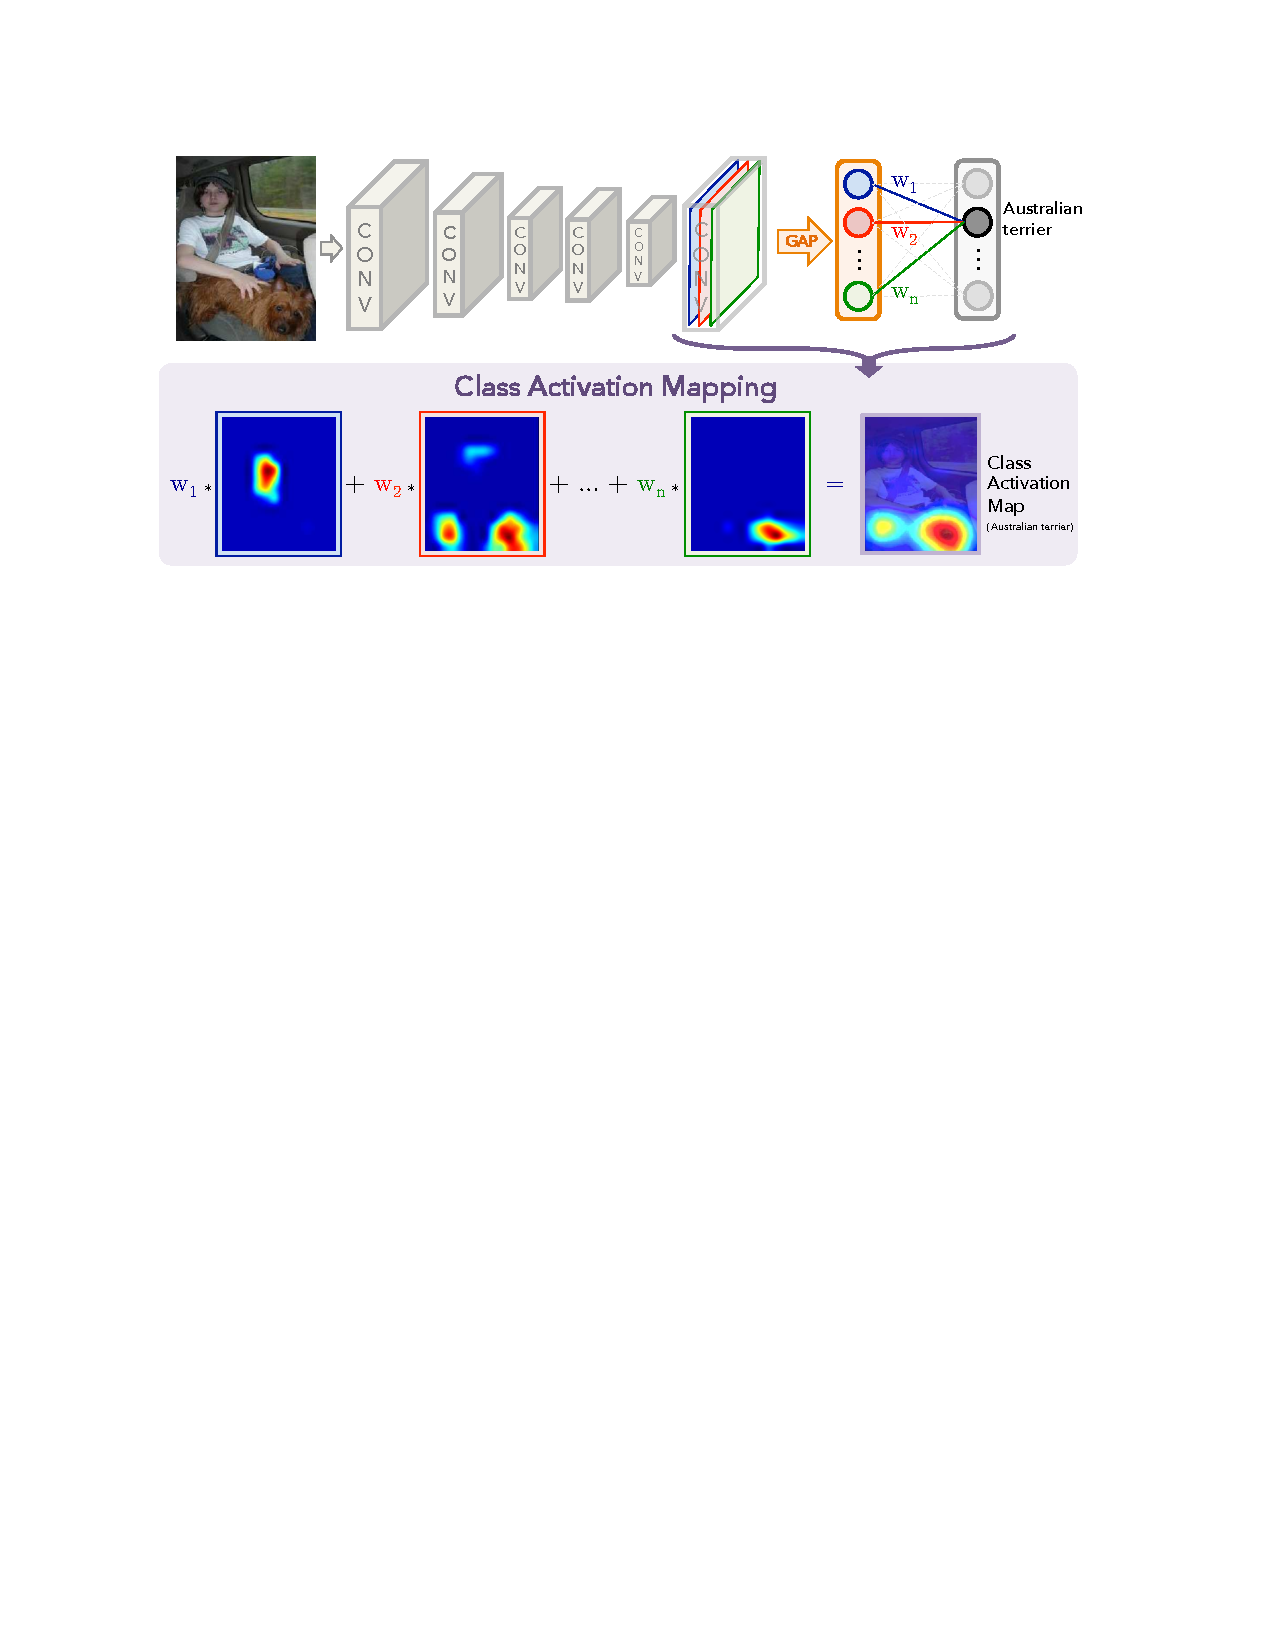
\includegraphics[width=.9\textwidth]{../graphics/Vis_CAM_principle.pdf}
  \source{adapted from \cite{Zhou:2016}}
\end{figure}
\begin{itemize}
\item In \cite{Zhou:2016}, the fully connected layers are replaced by Global Average Pooling (GAP). 
\item The final prediction is then made from the $n$-dimensional vector. The training provides us with a $n$-dimensional weight vector $w^c$ for each class. 
\end{itemize}
\end{frame}

\begin{frame}{Class Activation Mapping (CAM)}
\begin{itemize}
\item More formally, if the last convolutional layer has $n$ feature maps, GAP maps this layer to a $n$-dimensional vector: 
\begin{equation}
	GAP(k) = \frac{1}{N}\sum_{i,j}f_k(i,j) \quad \quad k = 1, \ldots, n
\end{equation}
where $N$ is the number of neurons in each feature map and $n$ the number of feature maps.
\item The score $S_c$ for each class $c$ is then the weighted sum of the vector entries:
\begin{equation}
	S_c = \sum_k w_k^c GAP(k)
\end{equation}
\item The posterior probabilities are obtained by softmax:
\begin{equation}
	P(c \, | \, x) = \frac{\exp{(S_c)}}{\sum_c \exp{(S_c)}}
\end{equation}
\item This modified network is then fine-tuned. Often, this simplification is not affecting classification accuracy very seriously \cite{Zhou:2016}. 
\end{itemize}
\end{frame}

\begin{frame}{Class Activation Mapping (CAM)}
\begin{itemize}
	\item The class scores can be written as:
	\begin{equation}
	S_c = \sum_k w_k^c \frac{1}{N}\sum_{i,j}f_k(i,j) = \frac{1}{N}\sum_{i,j} \sum_k w_k^c f_k(i,j) = \frac{1}{N}\sum_{i,j} M_c(i,j)
	\end{equation}
	$M_c$ is a class activation map, which is the weighted average of the last convolutional layer, with the weights optimized for prediction. 
	\item In practice, we might decide not to take the last convolutional layer, but one that is more upstream in order to get better spatial resolution. 
	\item In order to overlay to the original image, we simply upscale (interpolation). 
\end{itemize}
\end{frame}

\begin{frame}{Class Activation Mapping (CAM) - Results}
\begin{figure}[htb]
  \centering
  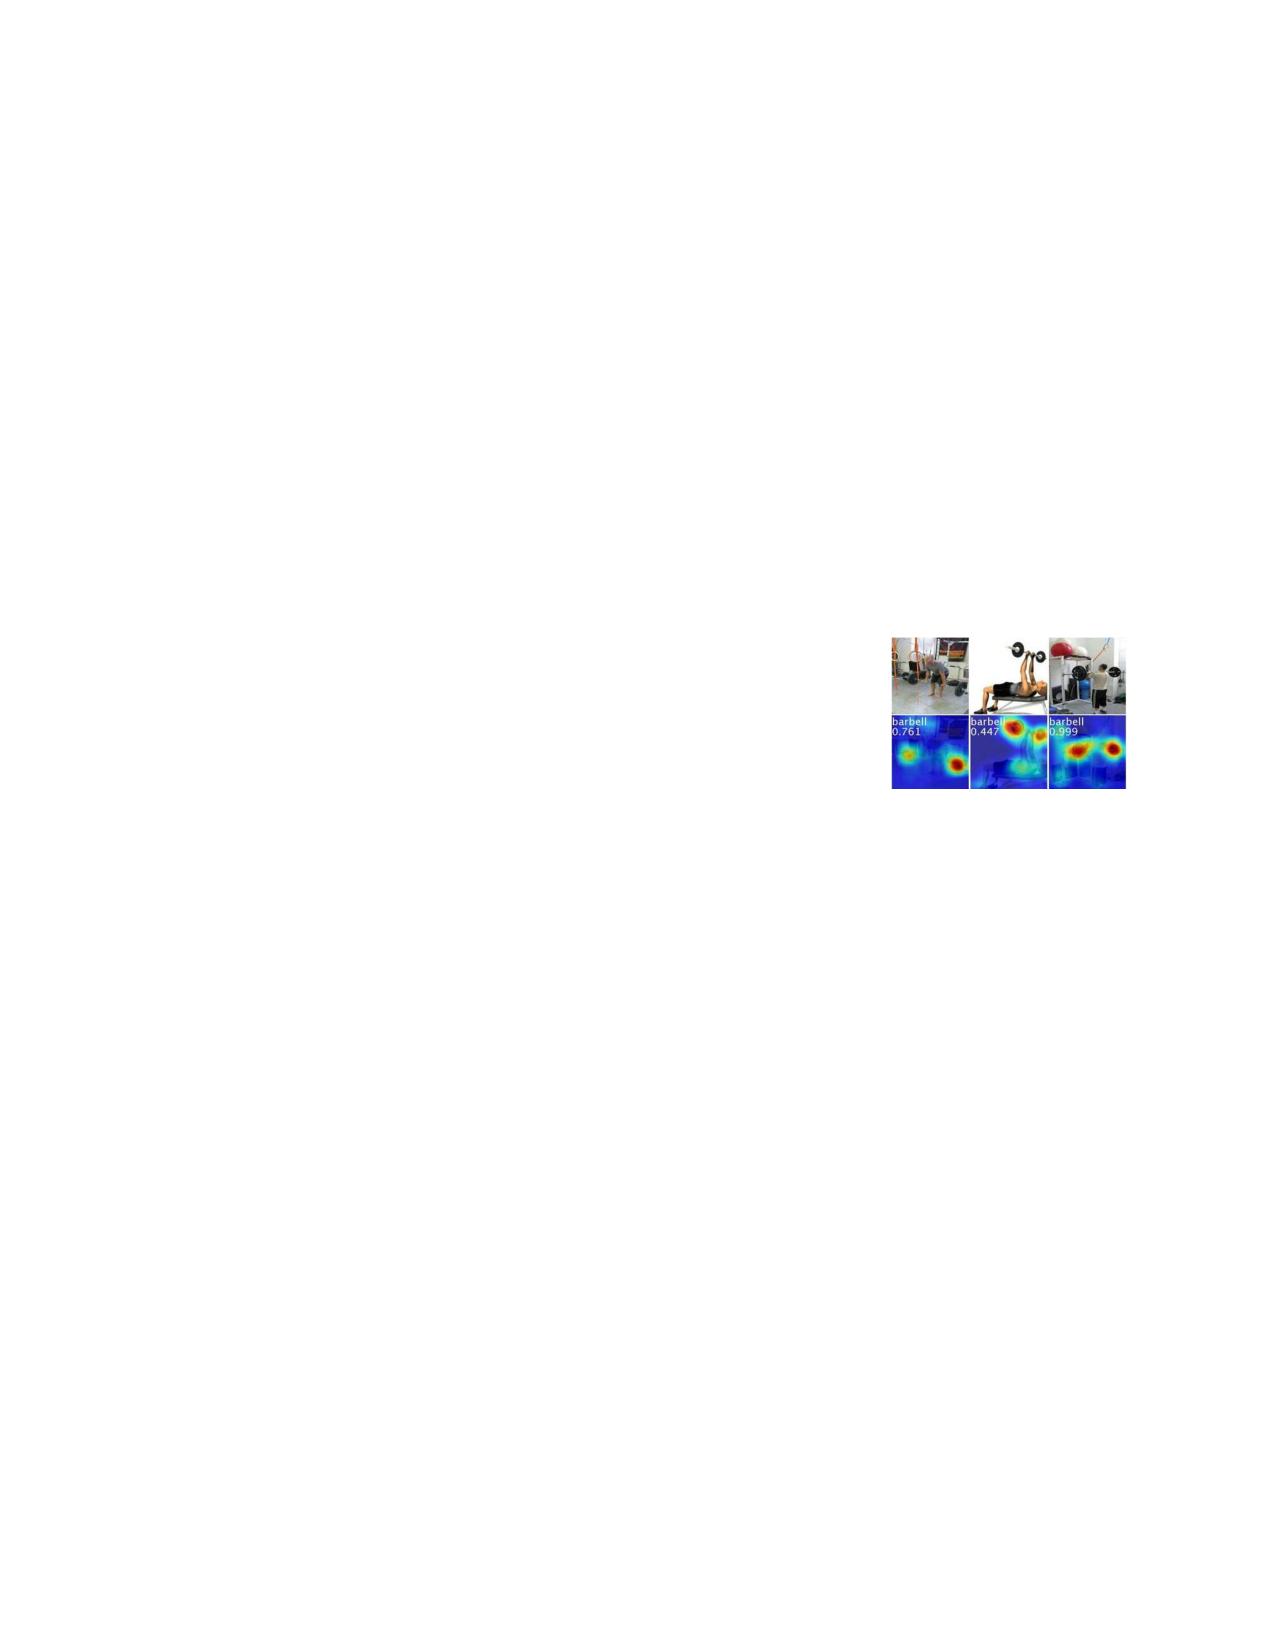
\includegraphics[width=.8\textwidth]{../graphics/Vis_CAM_Barbell.pdf}
  \source{adapted from \cite{Zhou:2016}}
\end{figure}
We see that the CAM highlights the regions which are discriminative for the predicted class ("barbell"). 
\end{frame}

\begin{frame}{Class Activation Mapping (CAM) - Results}
\begin{figure}[htb]
  \centering
  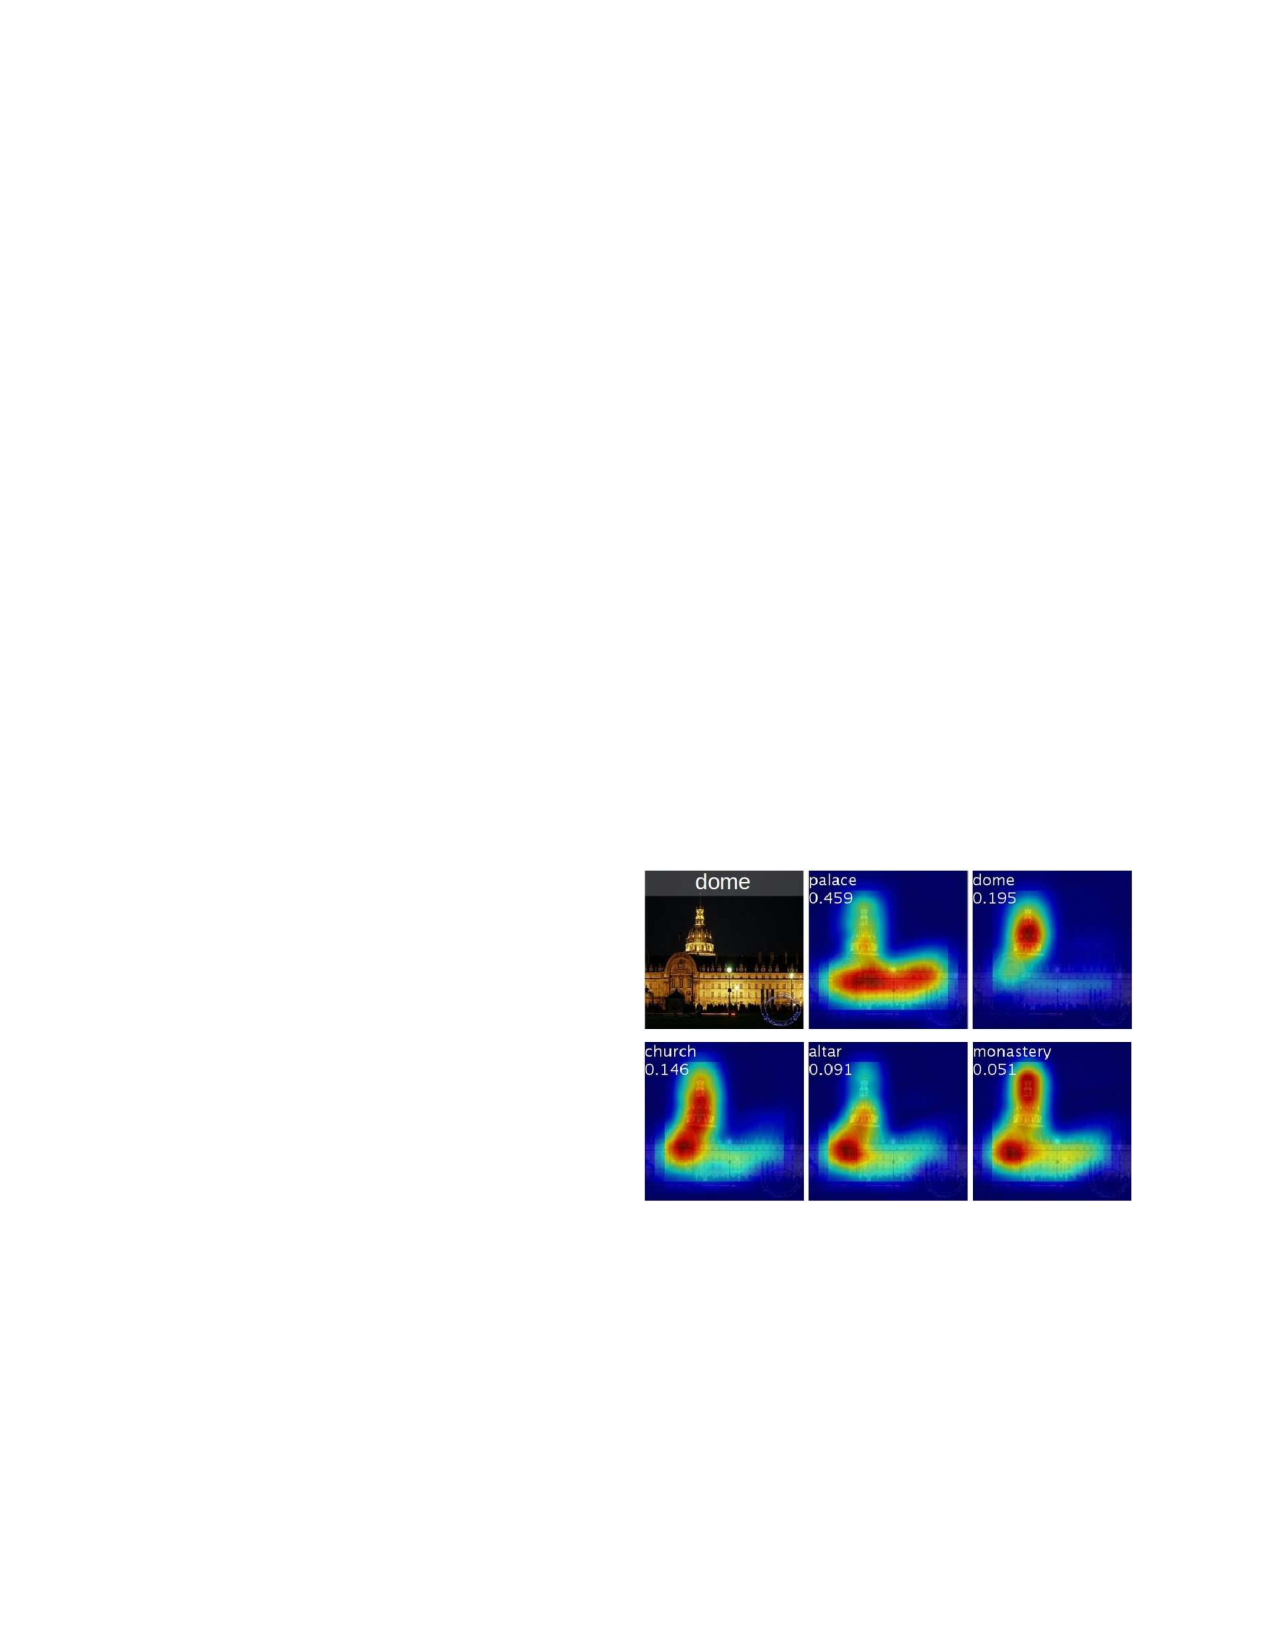
\includegraphics[width=.8\textwidth]{../graphics/Vis_CAM_Dome.pdf}
  \source{Image taken from  \cite{Zhou:2016}}
\end{figure}
We observe the variation of the CAM according to the predicted label. Here the correct label would have been "Dome". 
\end{frame}

\begin{frame}{Generalization of CAM: Grad-CAM}
\begin{itemize}
	\item A drawback of CAM is that we are not really analyzing a given network, but we design a similar network that we can then analyze. 
	\item This can be avoided by grad-CAM \cite{Selvaraju:2020}, that is based on the evaluation of gradients:
	\begin{equation}
		\alpha_k^c = \frac{1}{N}\sum_{i,j} \frac{\partial S_c}{\partial f_k(i,j)}
	\end{equation}
	\item If the fully connected layer is replaced by a global average pooling, this is identical to the $w_k^c$ we have calculated in CAM (up to a constant factor). 
	\item The final map is then calculated by:
	\begin{equation}
	M^{gradCAM}(c) = ReLu(\sum_k \alpha_k^c f_k)
	\end{equation}
	The ReLu is used to only account for positive contributions. 
\end{itemize}
\end{frame}

\begin{frame}{Grad-CAM results}
\begin{figure}[htb]
  \centering
  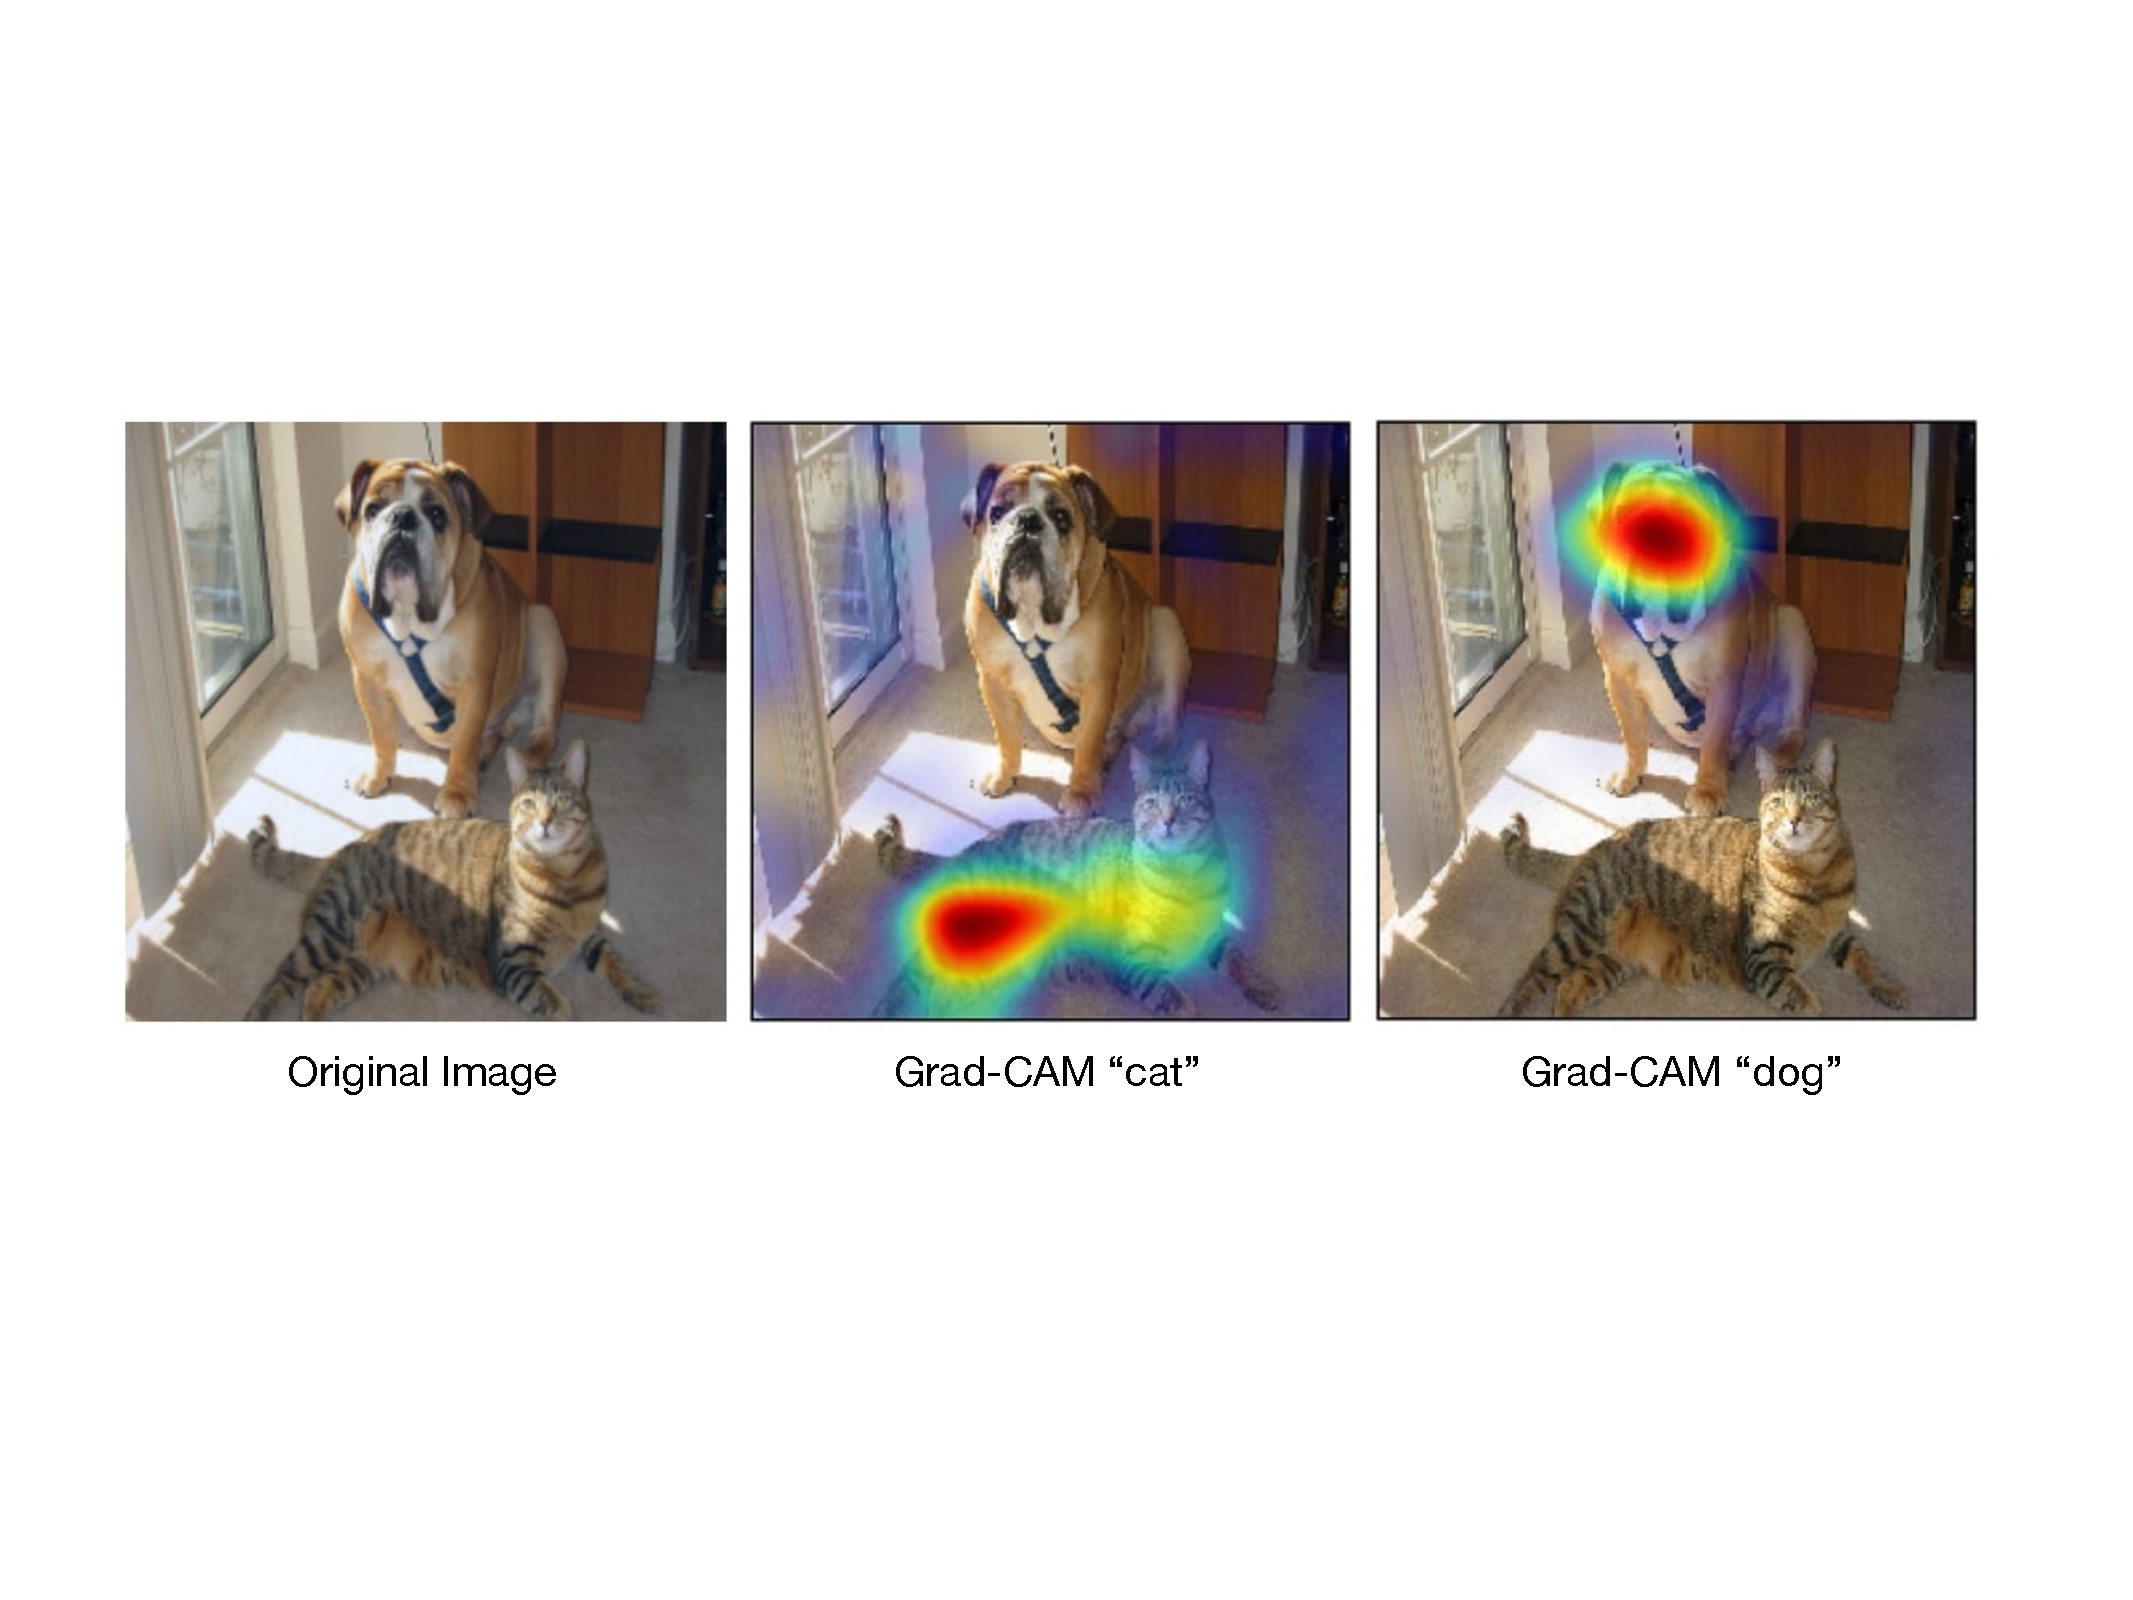
\includegraphics[width=.7\textwidth]{../graphics/Vis_GRADCAM_cat_and_dog.pdf}
  \source{adapted from \cite{Selvaraju:2020}}
\end{figure}
Grad-CAM result for an image with double label ("tiger-cat" and "boxer"). 
\end{frame}

\begin{frame}{Grad-CAM results: counter-factual image regions}
\begin{figure}[htb]
  \centering
  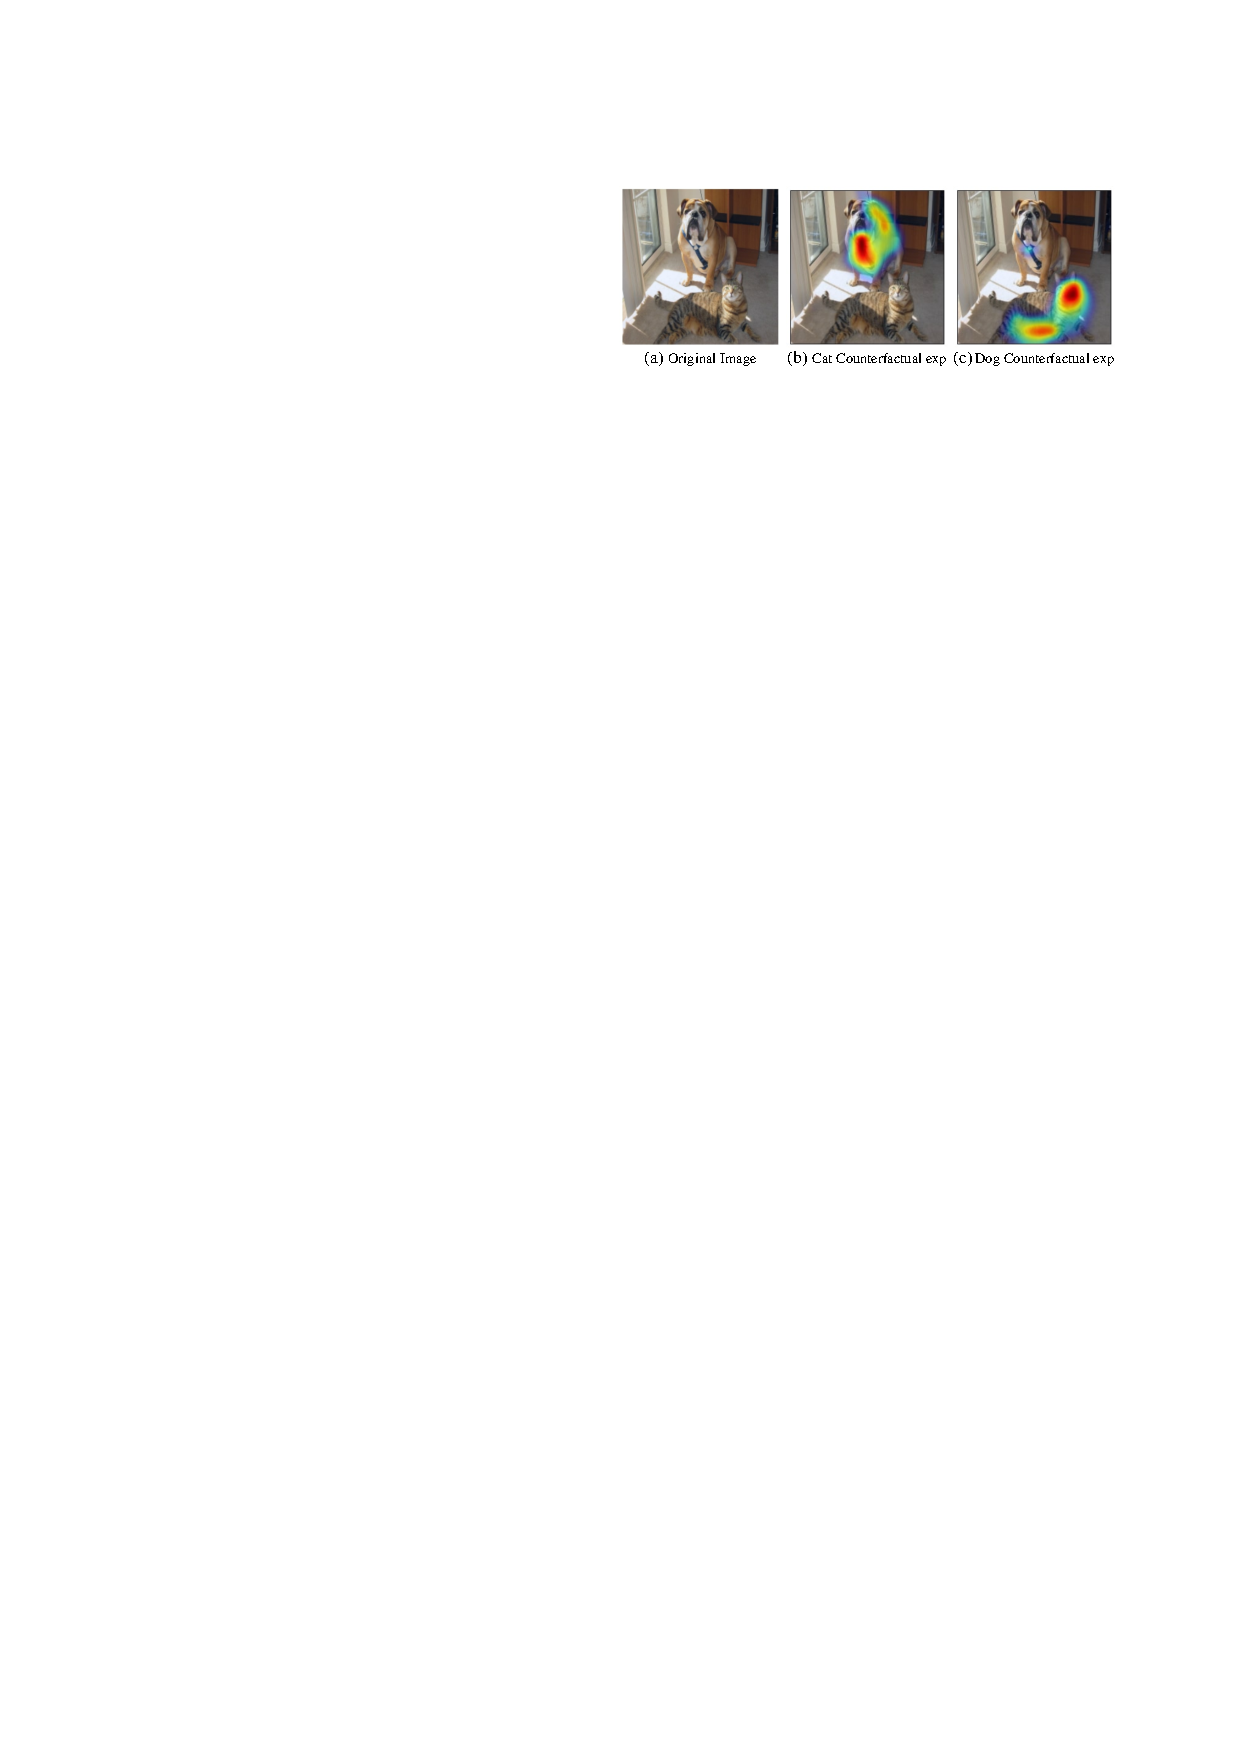
\includegraphics[width=.7\textwidth]{../graphics/Vis_GRADCAM_Counter.pdf}
  \source{adapted from \cite{Selvaraju:2020}}
\end{figure}
Here, the authors investigated which regions would rather make the network change its prediction. This is simply done by inverting the sign: 
\begin{equation}
	\alpha_k^c = \frac{1}{N}\sum_{i,j} -\frac{\partial S_c}{\partial f_k(i,j)}
\end{equation}
\end{frame}

\begin{frame}{Grad-CAM results: spotting bias}
\begin{figure}[htb]
  \centering
  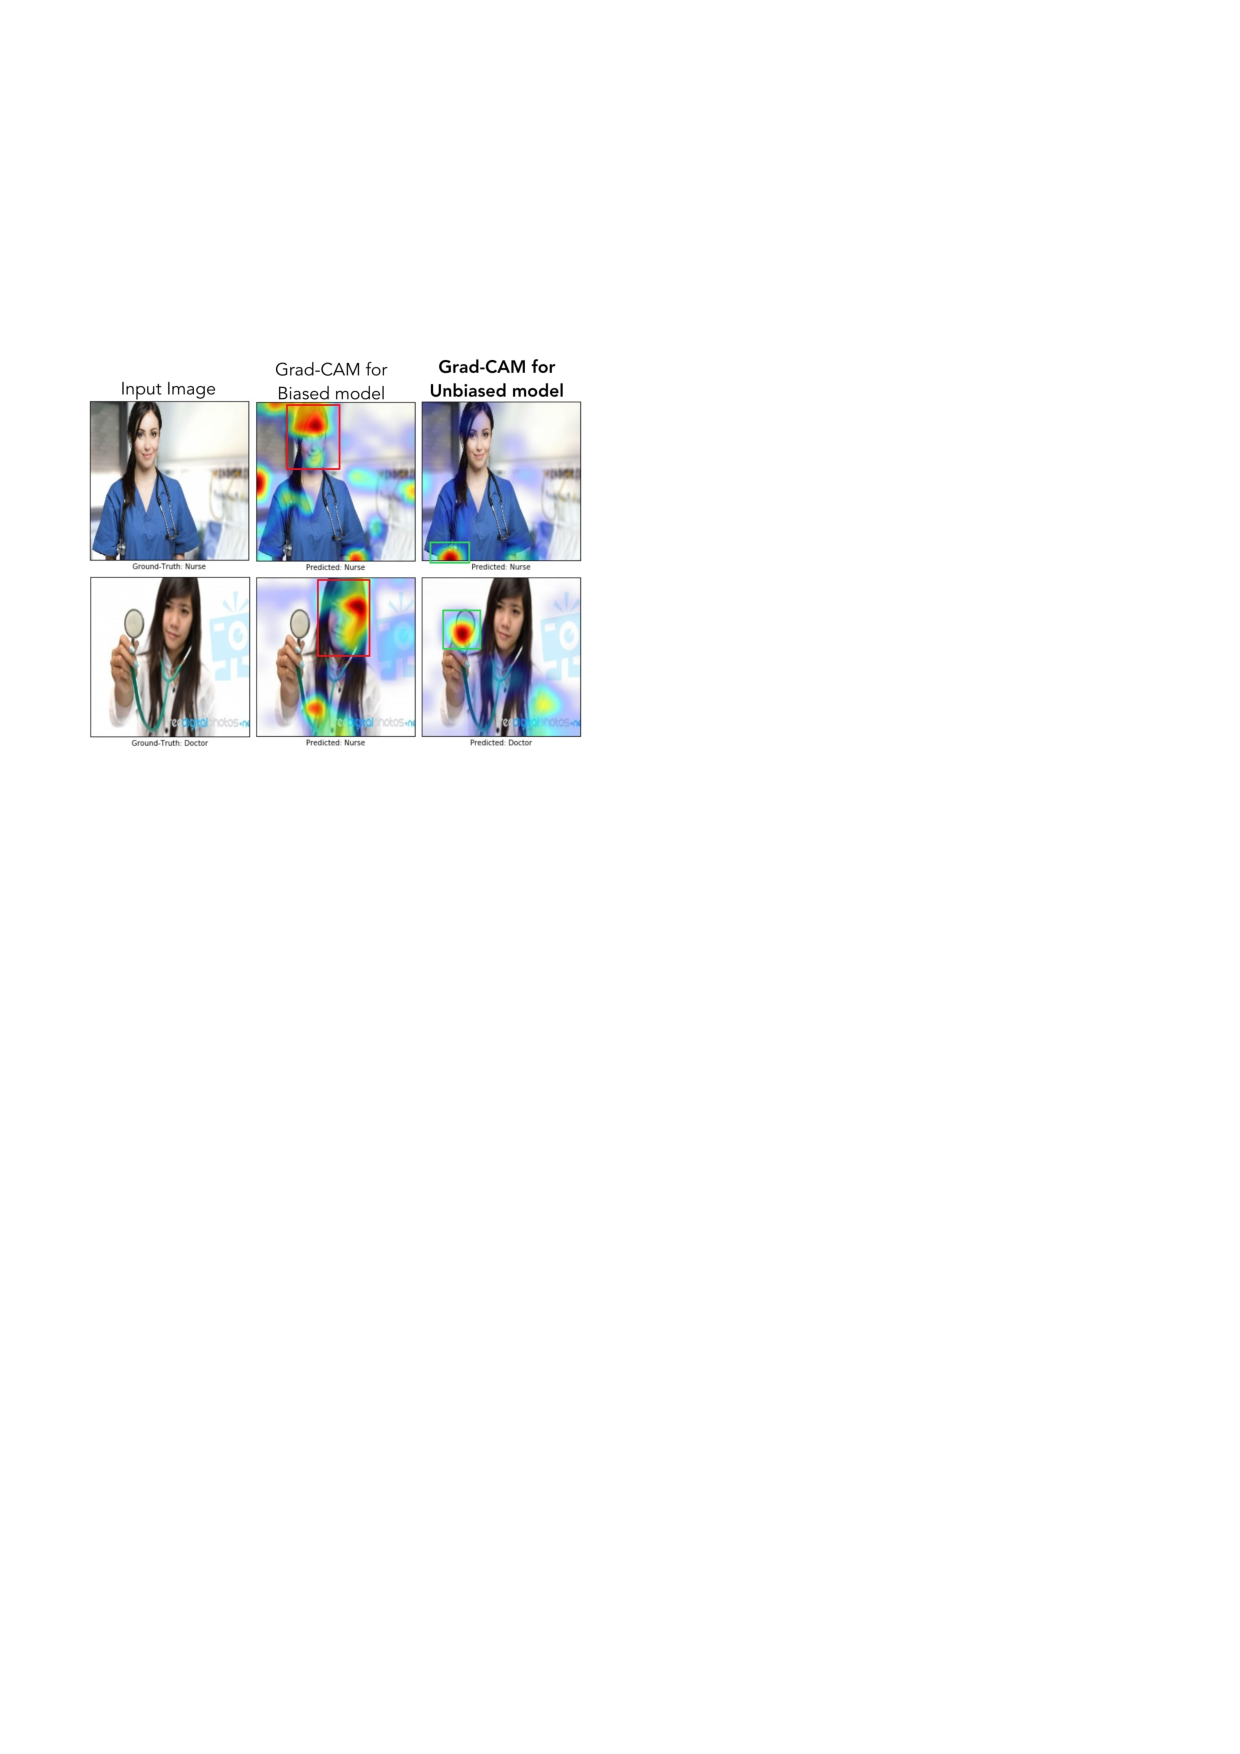
\includegraphics[width=.6\textwidth]{../graphics/Vis_GRADCAM_bias.pdf}
  \source{adapted from \cite{Selvaraju:2020}}
\end{figure}
In \cite{Selvaraju:2020}, a neural network was trained to distinguish between two classes "Nurse" and "Doctor". 
The training set contained a gender bias. We see that the important regions differ when the bias is removed.
%We see that the decision was then made according to regions in the face and hair. For the unbiased version, the decision was based on the coat color, the sleeves and the stethoscope. 
\end{frame}

\begin{frame}{Maximally activating images}
\begin{itemize}
	\item Another strategy is to generate an image that maximizes a particular neuron, typically a class score:
	\begin{equation}
	X^{\ast} = \argmax_{X} S_c(X) - \lambda \|X\|^2
	\end{equation}
	\item This can be achieved by a similar technique as training the network, but this time the parameters of the network are fixed and the image is adapted as to maximize the objective function. 
	\item Here, we do not optimize the softmax, but the class score, as the softmax contains contributions from all classes. 
\end{itemize}
\end{frame}

\begin{frame}{Maximally activating images - Results}
\begin{figure}[htb]
  \centering
  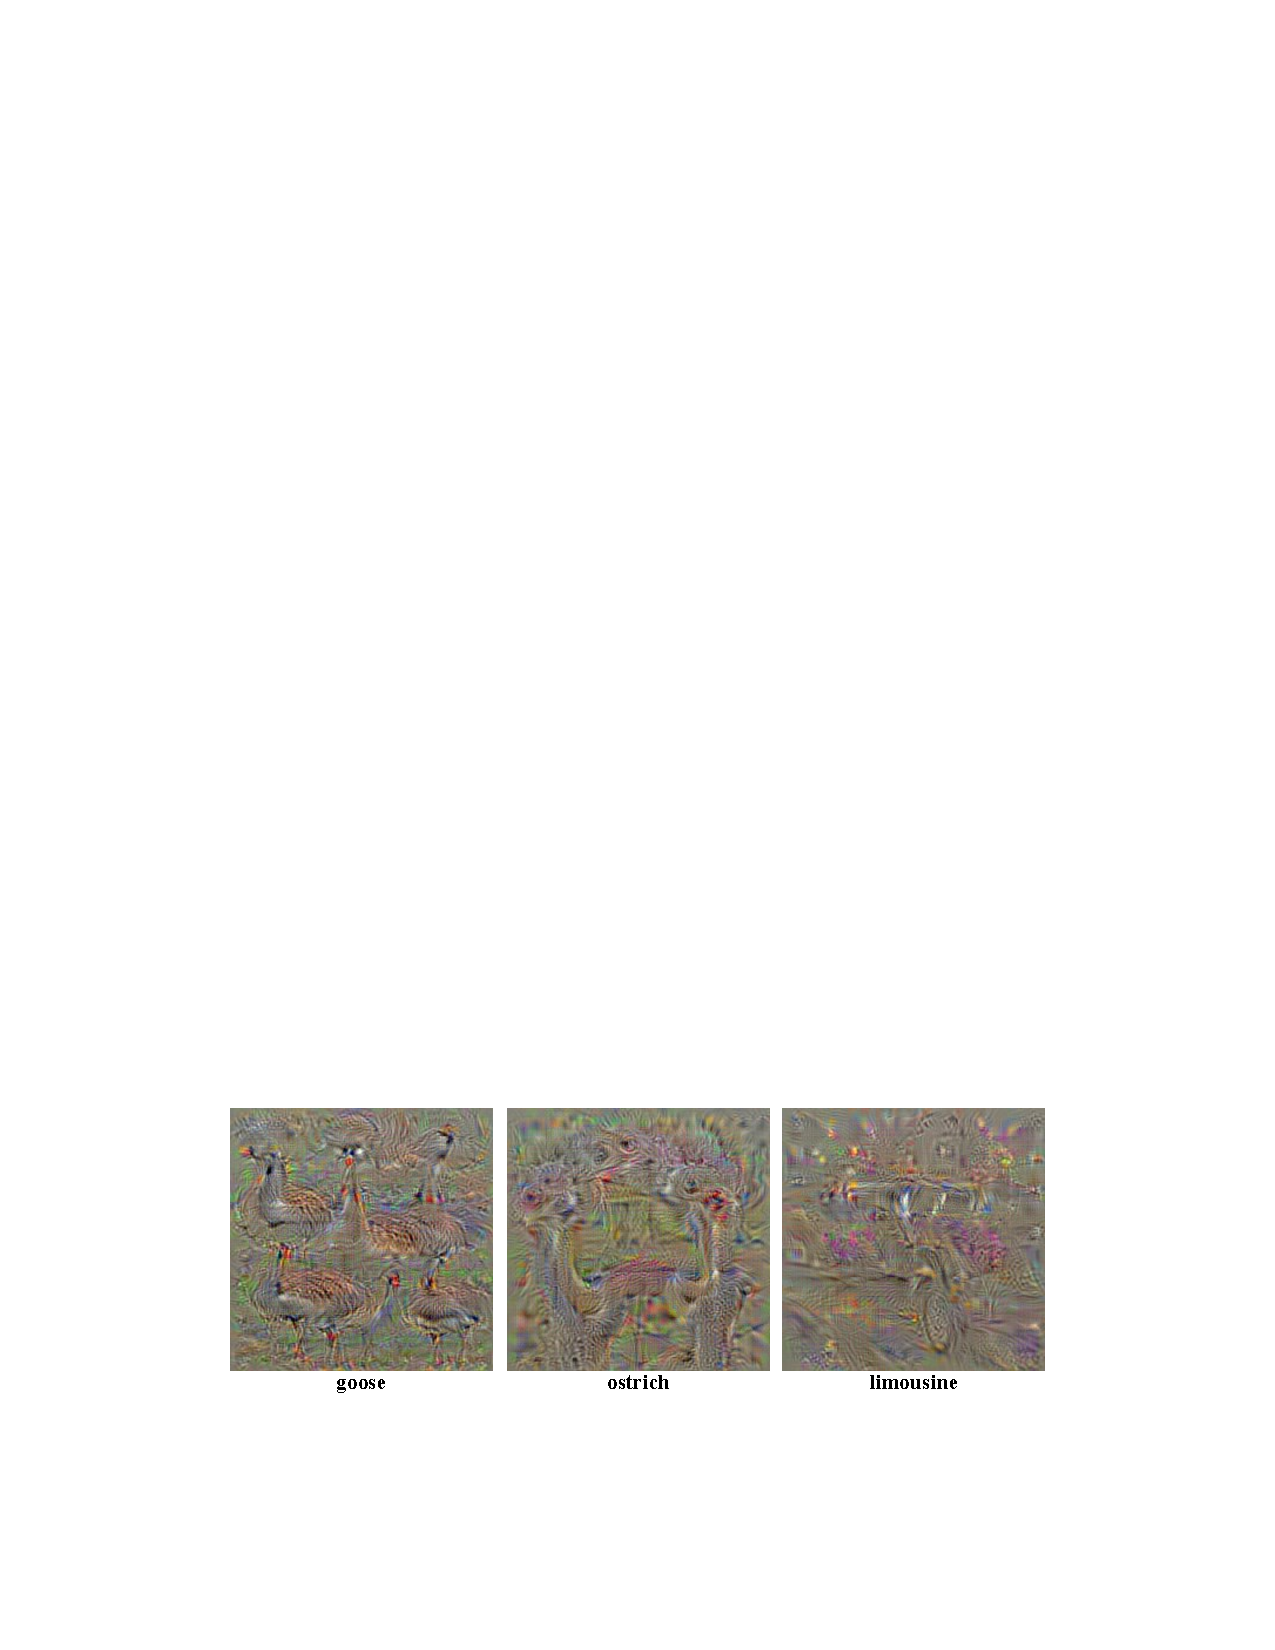
\includegraphics[width=.9\textwidth]{../graphics/Vis_dream.pdf}
  \source{adapted from \cite{Simonyan:2014}}
\end{figure}
We observe various elements the network is trained to react on.
\end{frame}

\begin{frame}{Application in digital pathology 1/2}
\begin{itemize}
	\item Task: grading cervix cancer according to severity
	\item Input data: stained tissue sections from biopsies or surgical specimen. 
	\item Multi-class-classification problem: (1) normal, (2) low grade displasia, (3) high grade displasia, (4) carcinoma
	\item Challenging question: which morphological patterns trigger the decision?
\end{itemize}
\end{frame}

\begin{frame}{Application in digital pathology 2/2}
\begin{figure}[htb]
  \centering
  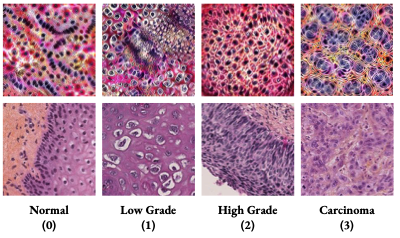
\includegraphics[width=.9\textwidth]{../graphics/Vis_max_activation_histopath.png}
  \source{adapted from \cite{Lubrano:2022}}
\end{figure}
\begin{itemize}
\item Maximally activating images are realistically looking images
\item The patterns correspond to known morphological hallmarks for grading.
\end{itemize}
\end{frame}



%%%%%%%%%%%%%%%%%%%%%%%%%%%%%%%%%%%%%%%%%%%%%%%%%%%%%%%%%%%%%%%%%%%%%%%%%
%%%%%%%%%%%%%%%%%%%%%%%%%%%%%%%%%%%%%%%%%%%%%%%%%%%%%%%%%%%%%%%%%%%%%%%%%
\section{Visualization of intermediate layers}
\frame{\frametitle{Overview}\tableofcontents[currentsection]}

\begin{frame}{Looking at activation maps}
   \begin{columns}
      \column{0.38\linewidth}
		\begin{figure}[htb]
				\centering
				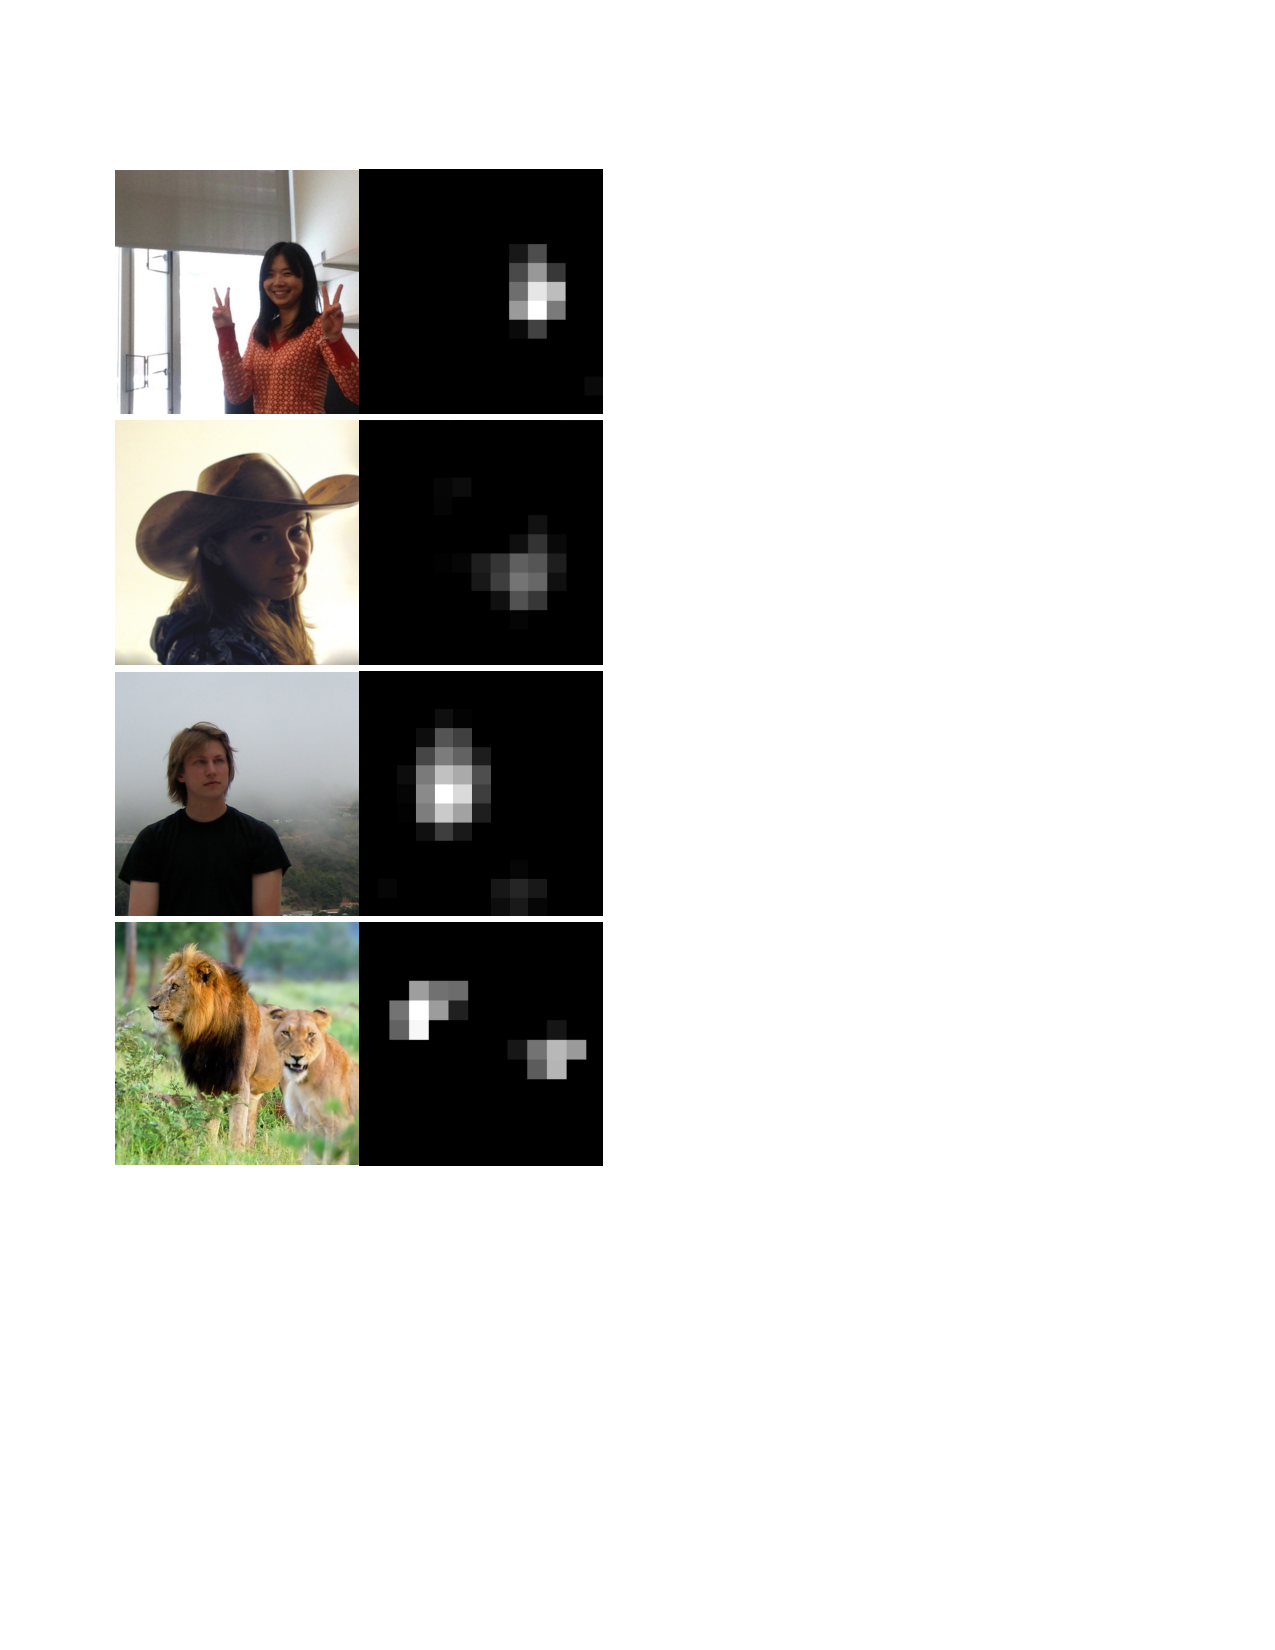
\includegraphics[width=3.5cm]{../graphics/Vis_looking_activation_maps.pdf}
		    \source{Image taken from \cite{Yosinski:2015}}
		\end{figure}

       \column{0.65\linewidth}
       \begin{itemize}
       		\item Simple visualization of activation maps inside the network. 
       		\item Example: channel 151 of conv5 layer. 
       		\item Sometimes, the information is very local, i.e. there are strong activations in one map of one layer (specialized map for text, faces, etc.)
       		\item Interestingly, there was no specific face class in the data set.
       		\item There are tools to perform these visualizations efficiently \cite{Yosinski:2015}.
       \end{itemize}
     \end{columns} 
\end{frame}


\begin{frame}{Mapping activation maps to the original pixel space}
\begin{figure}[htb]
  \centering
  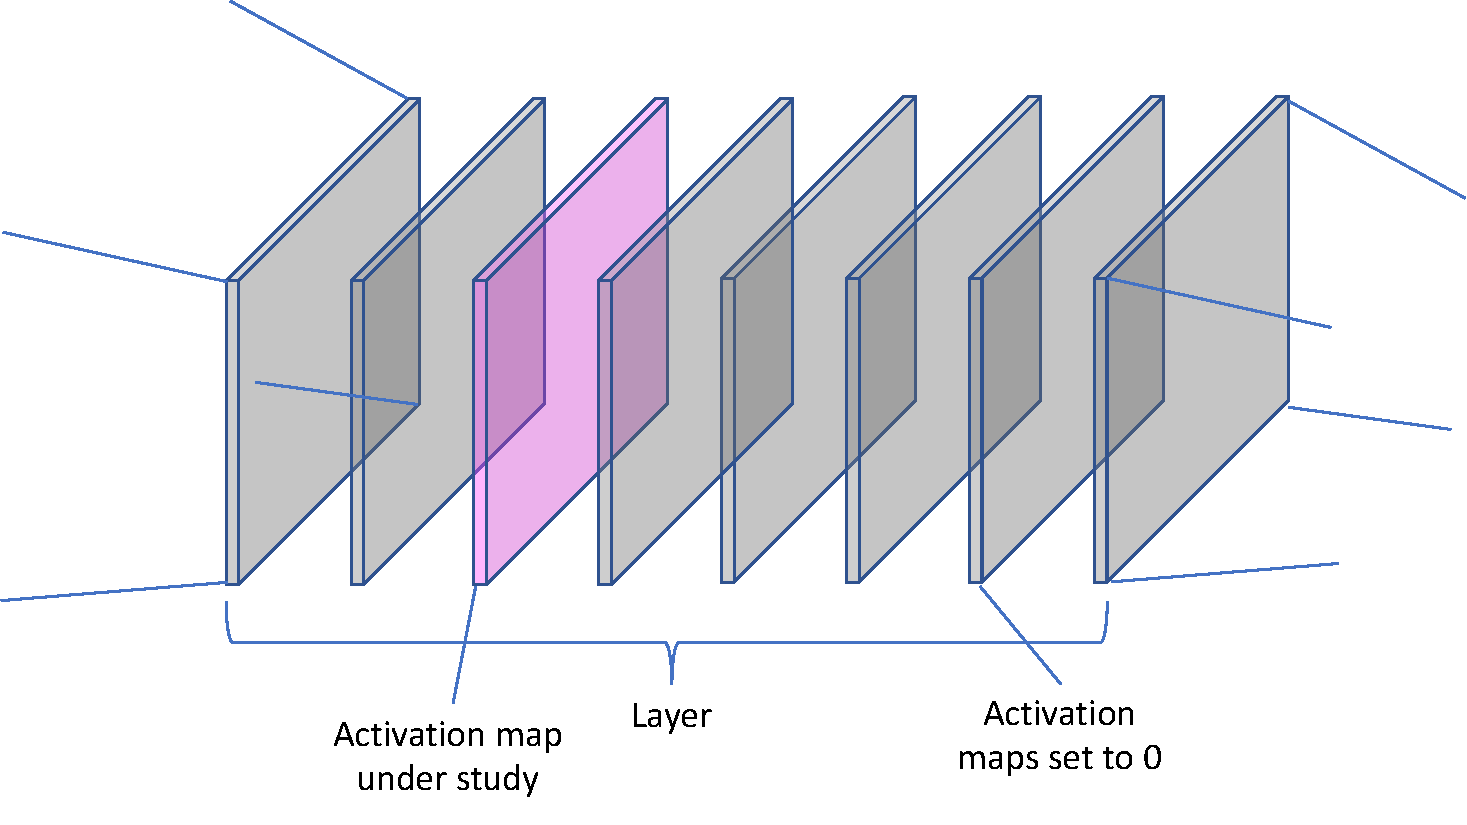
\includegraphics[width=.7\textwidth]{../graphics/Vis_activationmaps_zero.pdf}
\end{figure}
\begin{itemize}
	\item We would also like to understand which patterns in the original image are important for a particular activation map.
	\item In this case, we need to map activities back to the input pattern that caused the activity \cite{Zeiler:2013}. 
	\begin{itemize}
		\item We set all other maps in the layer to 0. 
		\item We "revert" the neural network from the feature map by using a deconvnet \cite{Zeiler:2011}.
	\end{itemize}
\end{itemize}
\end{frame}

\begin{frame}{How to map activities back to input pixel space}
\begin{itemize}
	\item There are three operations that need to be "reversed": convolution, ReLu, max-pooling. 
	\item {\bf Deconvolution:} \cite{Zeiler:2013} propose to simply convolve the activation map at the upper level with the transposed learned filter. 
	\item {\bf ReLu:} The Relu cannot be reversed. \cite{Zeiler:2013}  propose to simply put a ReLu in the deconvolution path as to only keep positive contributions. 
	\item {\bf Unpooling:} Pooling operations cannot be reverted. The deconvnet remembers where the maximum pixels originated from in the corresponding convolutional network. 
\end{itemize}
\end{frame}

\begin{frame}{How to map activities back to input pixel space}
\begin{figure}[htb]
  \centering
  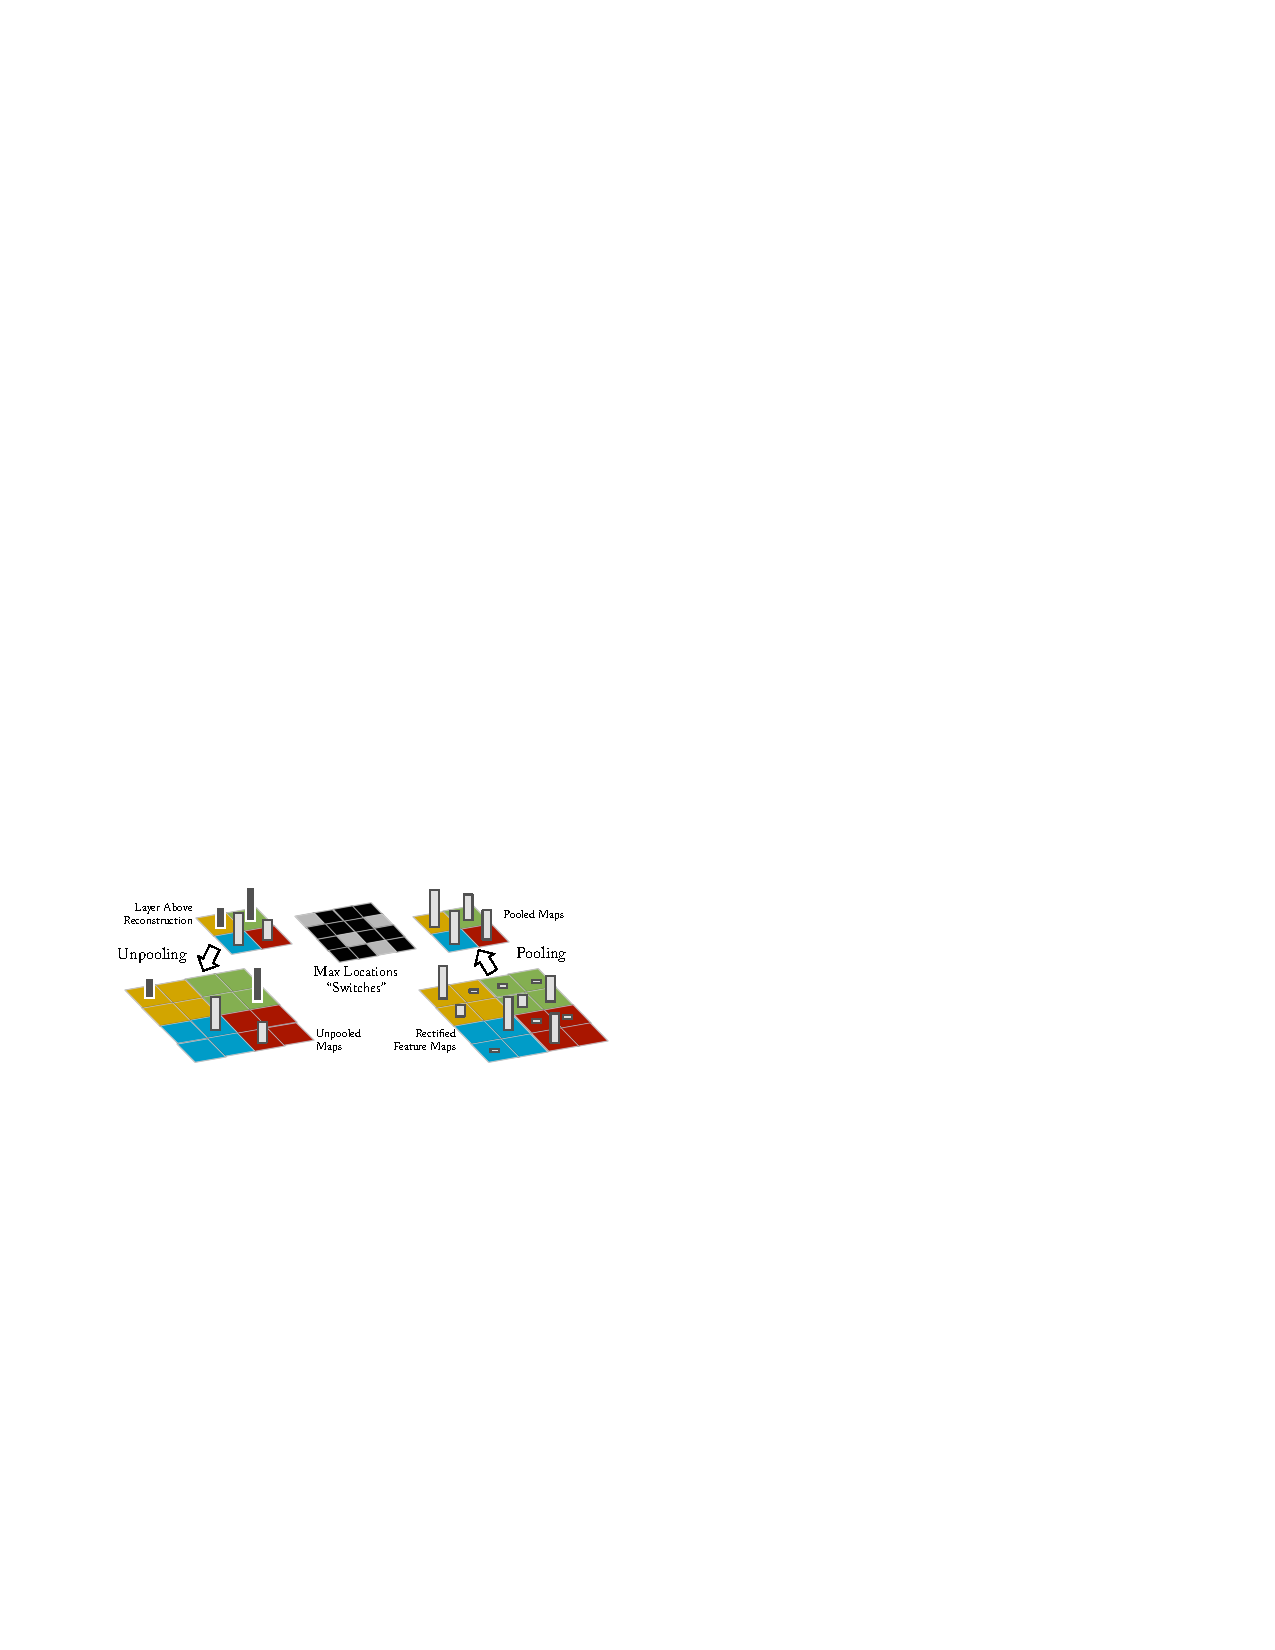
\includegraphics[width=.96\textwidth]{../graphics/Vis_unpooling2.pdf}
  \source{Image taken from \cite{Zeiler:2013}}
\end{figure}
% {\bf Unpooling:} 
% \begin{itemize}
% 	\item Pooling operations cannot be inverted (we lost the values that were discarded). 
% 	\item The deconvnet remembers where the maximum pixels originated from in the corresponding convolutional network. 
% \end{itemize}
\end{frame}

\begin{frame}{Experiments}
\begin{itemize}
	\item ImageNet Validation Set. 
	\item For a layer, a number of feature maps is (randomly) selected.
	\item For these feature maps, the 9 maximal activations are then reconstructed at the pixel level. 
	\item Both the reconstructed image and the original crops are visualized.
\end{itemize}
\end{frame}

\begin{frame}{Visualization of image features for layer 2 activation maps}
\begin{figure}[htb]
  \centering
  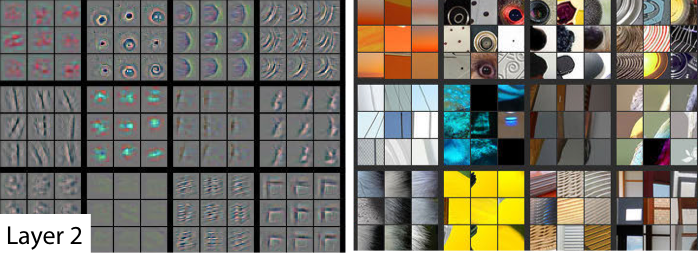
\includegraphics[width=\textwidth]{../graphics/Vis_Layer2_activationmaps.pdf}
\end{figure}
The top 9 activation maps with the strongest signal across the validation set for layer 2. \\
Layer 2 features are slightly more complex patterns (corners, bended contours, color combinations) than in layer 1, but still relatively basic.
\end{frame}

\begin{frame}{Visualization of image features for layer 3 activation maps}
\begin{figure}[htb]
  \centering
  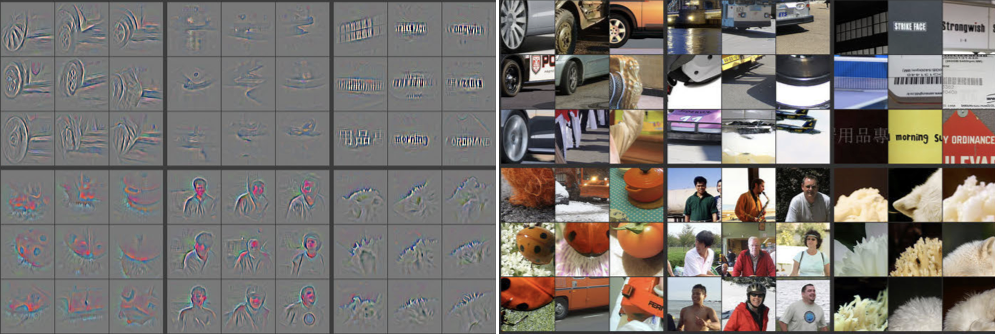
\includegraphics[width=\textwidth]{../graphics/Vis_Layer3_activationmaps.png}
\end{figure}
The top 9 activation maps with the strongest signal across the validation set for layer 3. \\
Higher Level features: faces, text, geometrical features.
\end{frame}

\begin{frame}{Visualization of image features for layer 5 activation maps}
\begin{figure}[htb]
  \centering
  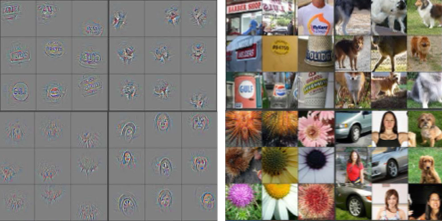
\includegraphics[width=\textwidth]{../graphics/Vis_Layer5_activationmaps.pdf}
\end{figure}
The top 9 projected activation maps for layer 5 across the validation set. \\
e.g. faces: contours, hair, nose ... 
\end{frame}

\begin{frame}{Visualization of image features for layer 5 activation maps}
\begin{figure}[htb]
  \centering
  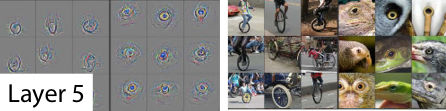
\includegraphics[width=\textwidth]{../graphics/Vis_Layer5_activationmaps_c.pdf}
\end{figure}
Here, we observe an eye detector and a wheel detector. \\
The image analysis community has developed many algorithms for eye detection; here the detection is implicit.
\end{frame}

\begin{frame}{Visualization of image features for layer 5 activation maps}
\begin{figure}[htb]
  \centering
  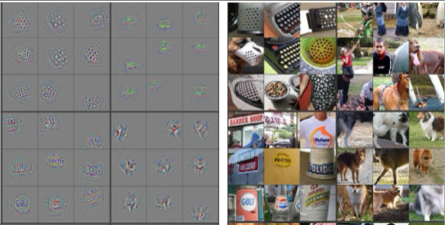
\includegraphics[width=\textwidth]{../graphics/Vis_Layer5_activationmaps_b.pdf}
\end{figure}
\begin{itemize}
\item <1-> Sometimes, the results can be surprising ... (top right)
\item <2-> We have a background grass detector. 
\end{itemize}
\end{frame}

\begin{frame}{Image features during training across different layers}
\begin{figure}[htb]
  \centering
  \subfloat{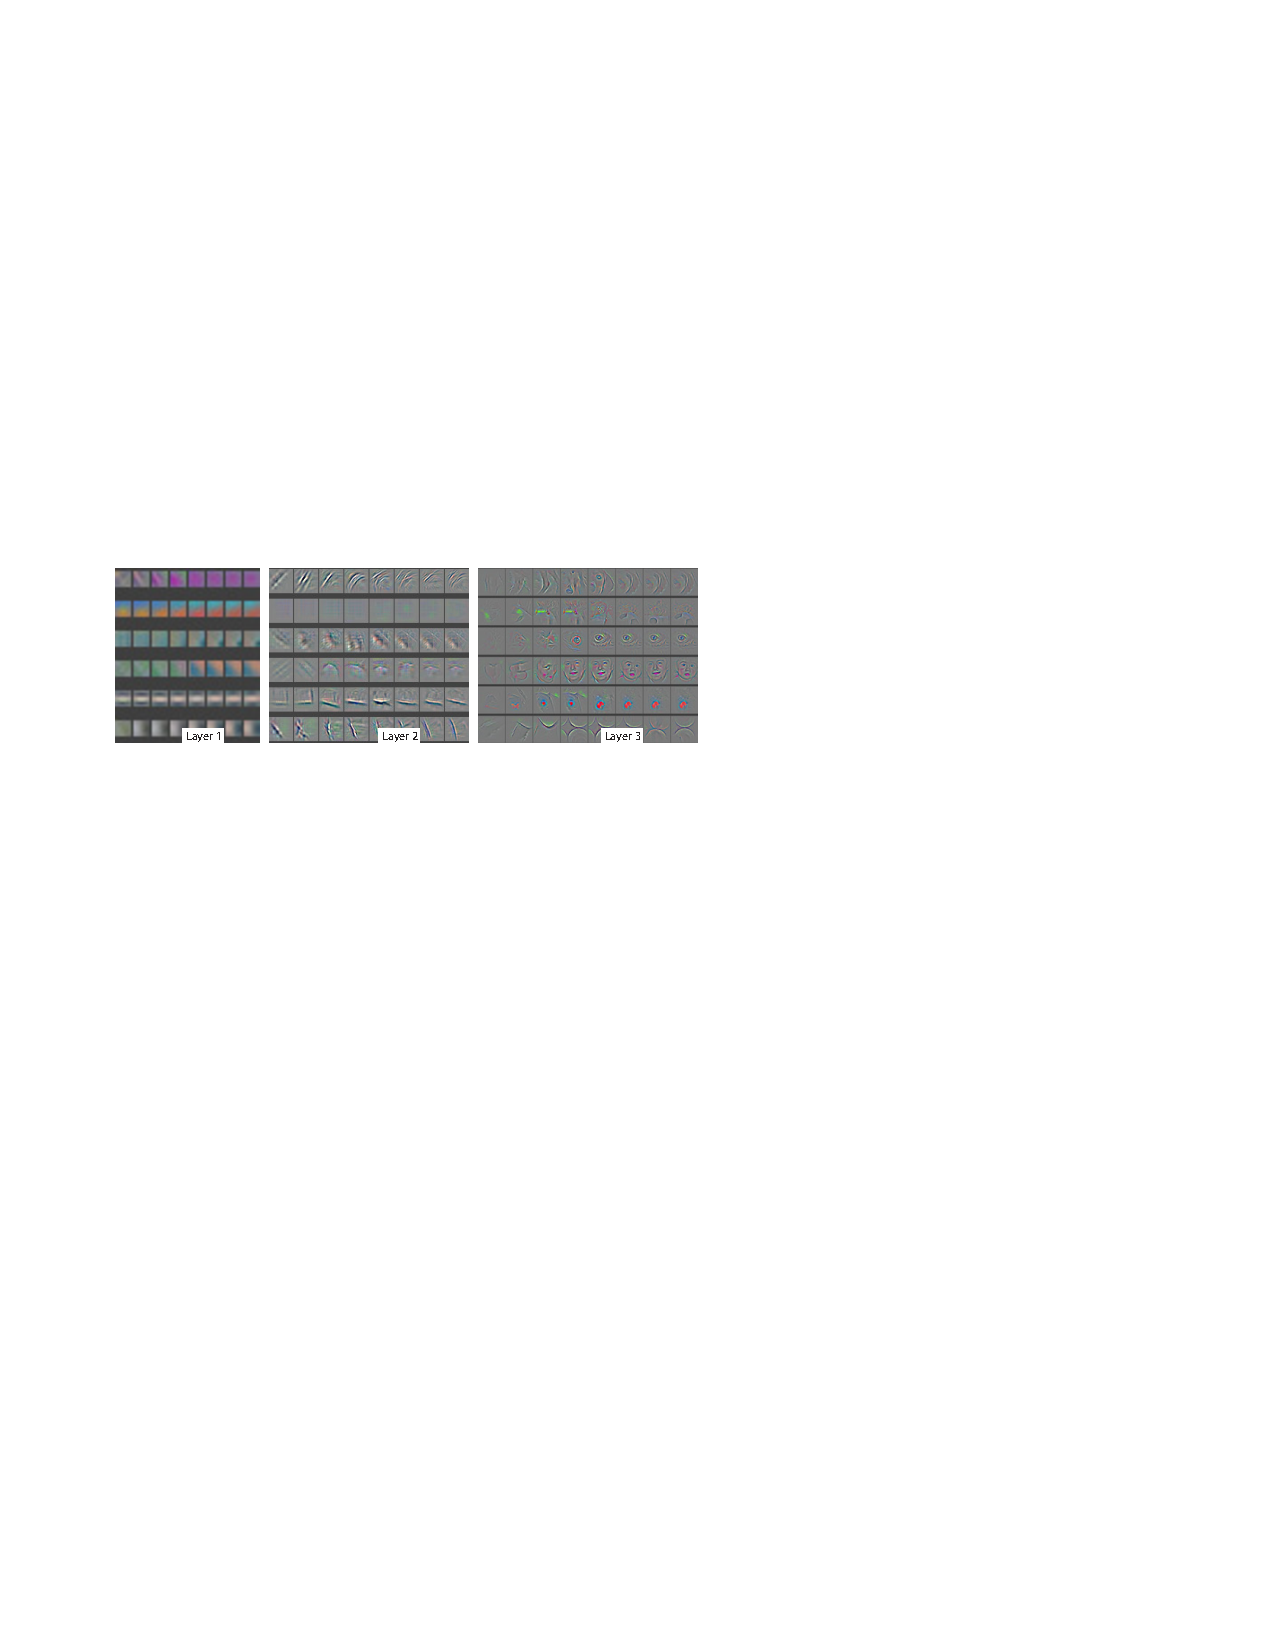
\includegraphics[height=.3\textheight]{../graphics/Vis_activationmaps_training1.pdf}}\\  
  \subfloat{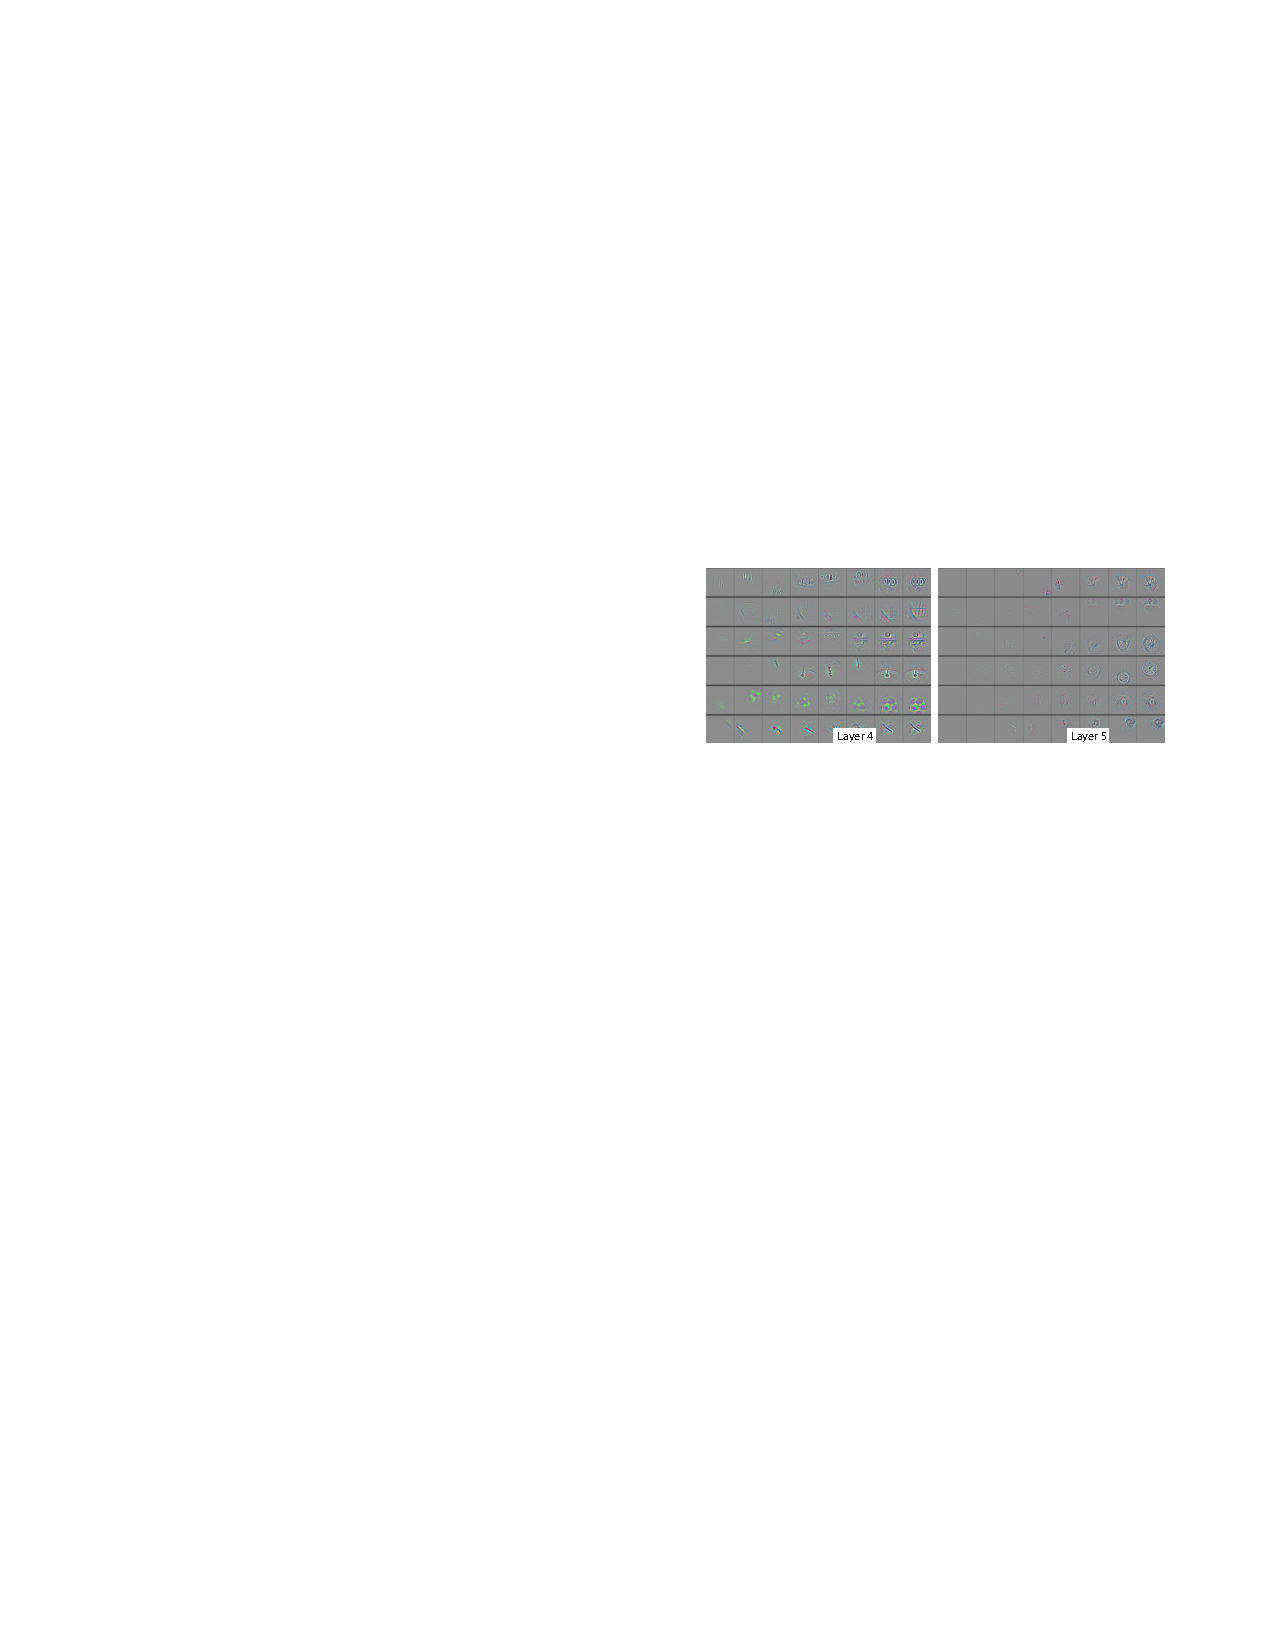
\includegraphics[height=.3\textheight]{../graphics/Vis_activationmaps_training2.pdf}} 
\end{figure}
\begin{itemize}
	\item <1-> Image features for activation maps depending on epochs. What do you observe?
	\item <2-> The lower level features are learned first (a few epochs). Higher level features take more time to converge.
\end{itemize}
\end{frame}

% \begin{frame}{Finding Image features by gradient ascent}
% An alternative approach is to find images by solving the following maximization problem \cite{Yosinski:2015}:
% \begin{equation*}
% x^{\ast} = \argmax_x a_i(\x) - R_{\param}(\x)
% \end{equation*}
% For a given activation map, we will find the "preferred" image, i.e. the image that would 
% \begin{figure}[htb]
%   \centering
%   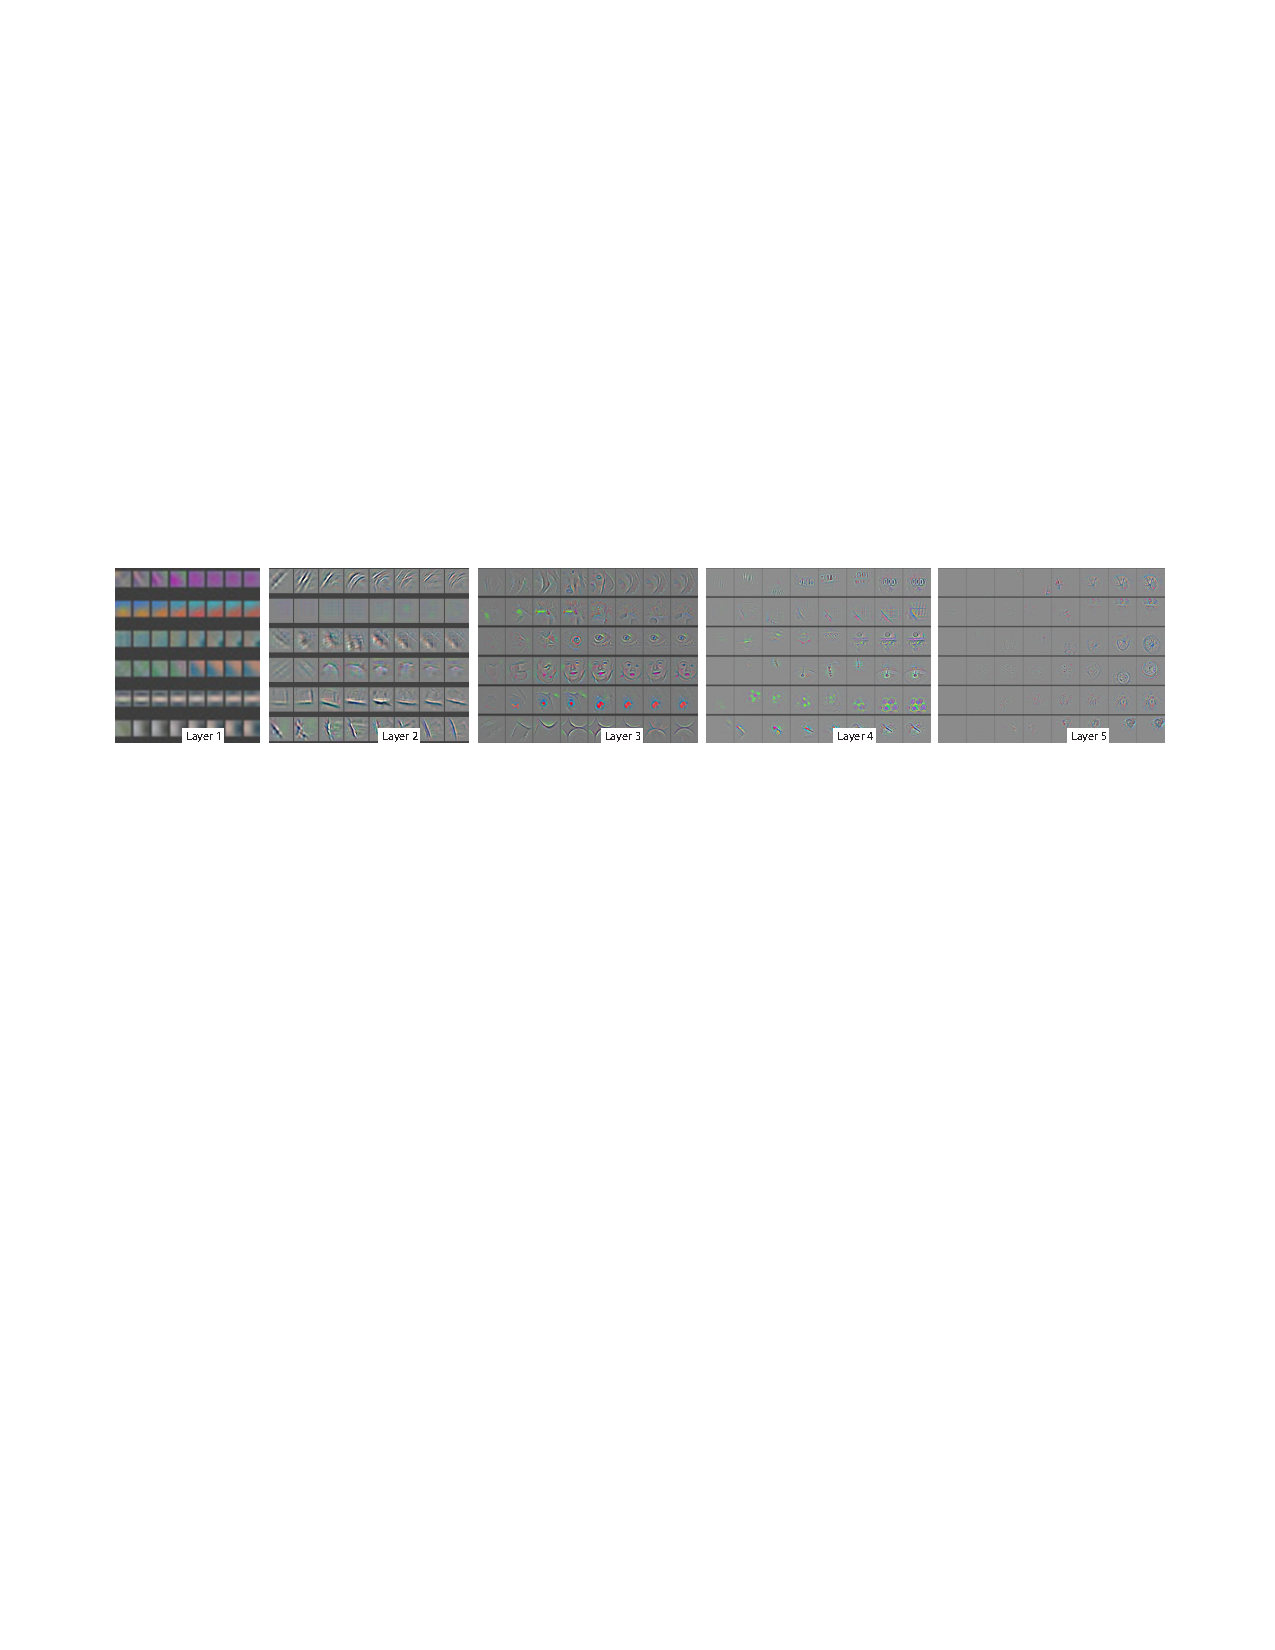
\includegraphics[width=\textwidth]{../graphics/Vis_activationmaps_training.pdf}
% \end{figure}
% \end{frame}

%%%%%%%%%%%%%%%%%%%%%%%%%%%%%%%%%%%%%%%%%%%%%%%%%%%%%%%%%%%%%%%%%%%%%%%%%
%%%%%%%%%%%%%%%%%%%%%%%%%%%%%%%%%%%%%%%%%%%%%%%%%%%%%%%%%%%%%%%%%%%%%%%%%
\section{Visualization of the loss function}
\frame{\frametitle{Overview}\tableofcontents[currentsection]}

\begin{frame}{Motivation: visualization of the loss function}
\begin{itemize}
	\item We have seen that training a Neural Networks corresponds to solving a minimization problem: 
	\begin{equation*}
		\param ^{\ast} = \argmin_{\param} \loss (\param) + \lambda \mathcal{R}(\param)
	\end{equation*}
	where $\param$ is the vector of all parameters, $\mathcal{R}(\param)$ a regularization term and $\loss (\param)$ the loss term calculated on the training data:
	\begin{equation*}
		\loss (\param) = \sum_{i=1}^N \loss_i (\param)
	\end{equation*}
	\item Visualization of the loss can give us a hint on how complicated this task really is. 
	\item Visualization can also allow us to compare different architectures or initialization schemes.
\end{itemize}
\end{frame}


%\begin{frame}{Spotting problems by visual inspection of the loss}
%\begin{itemize}
%\end{itemize}
%\end{frame}

\begin{frame}{Convexity}
\begin{figure}[htb]
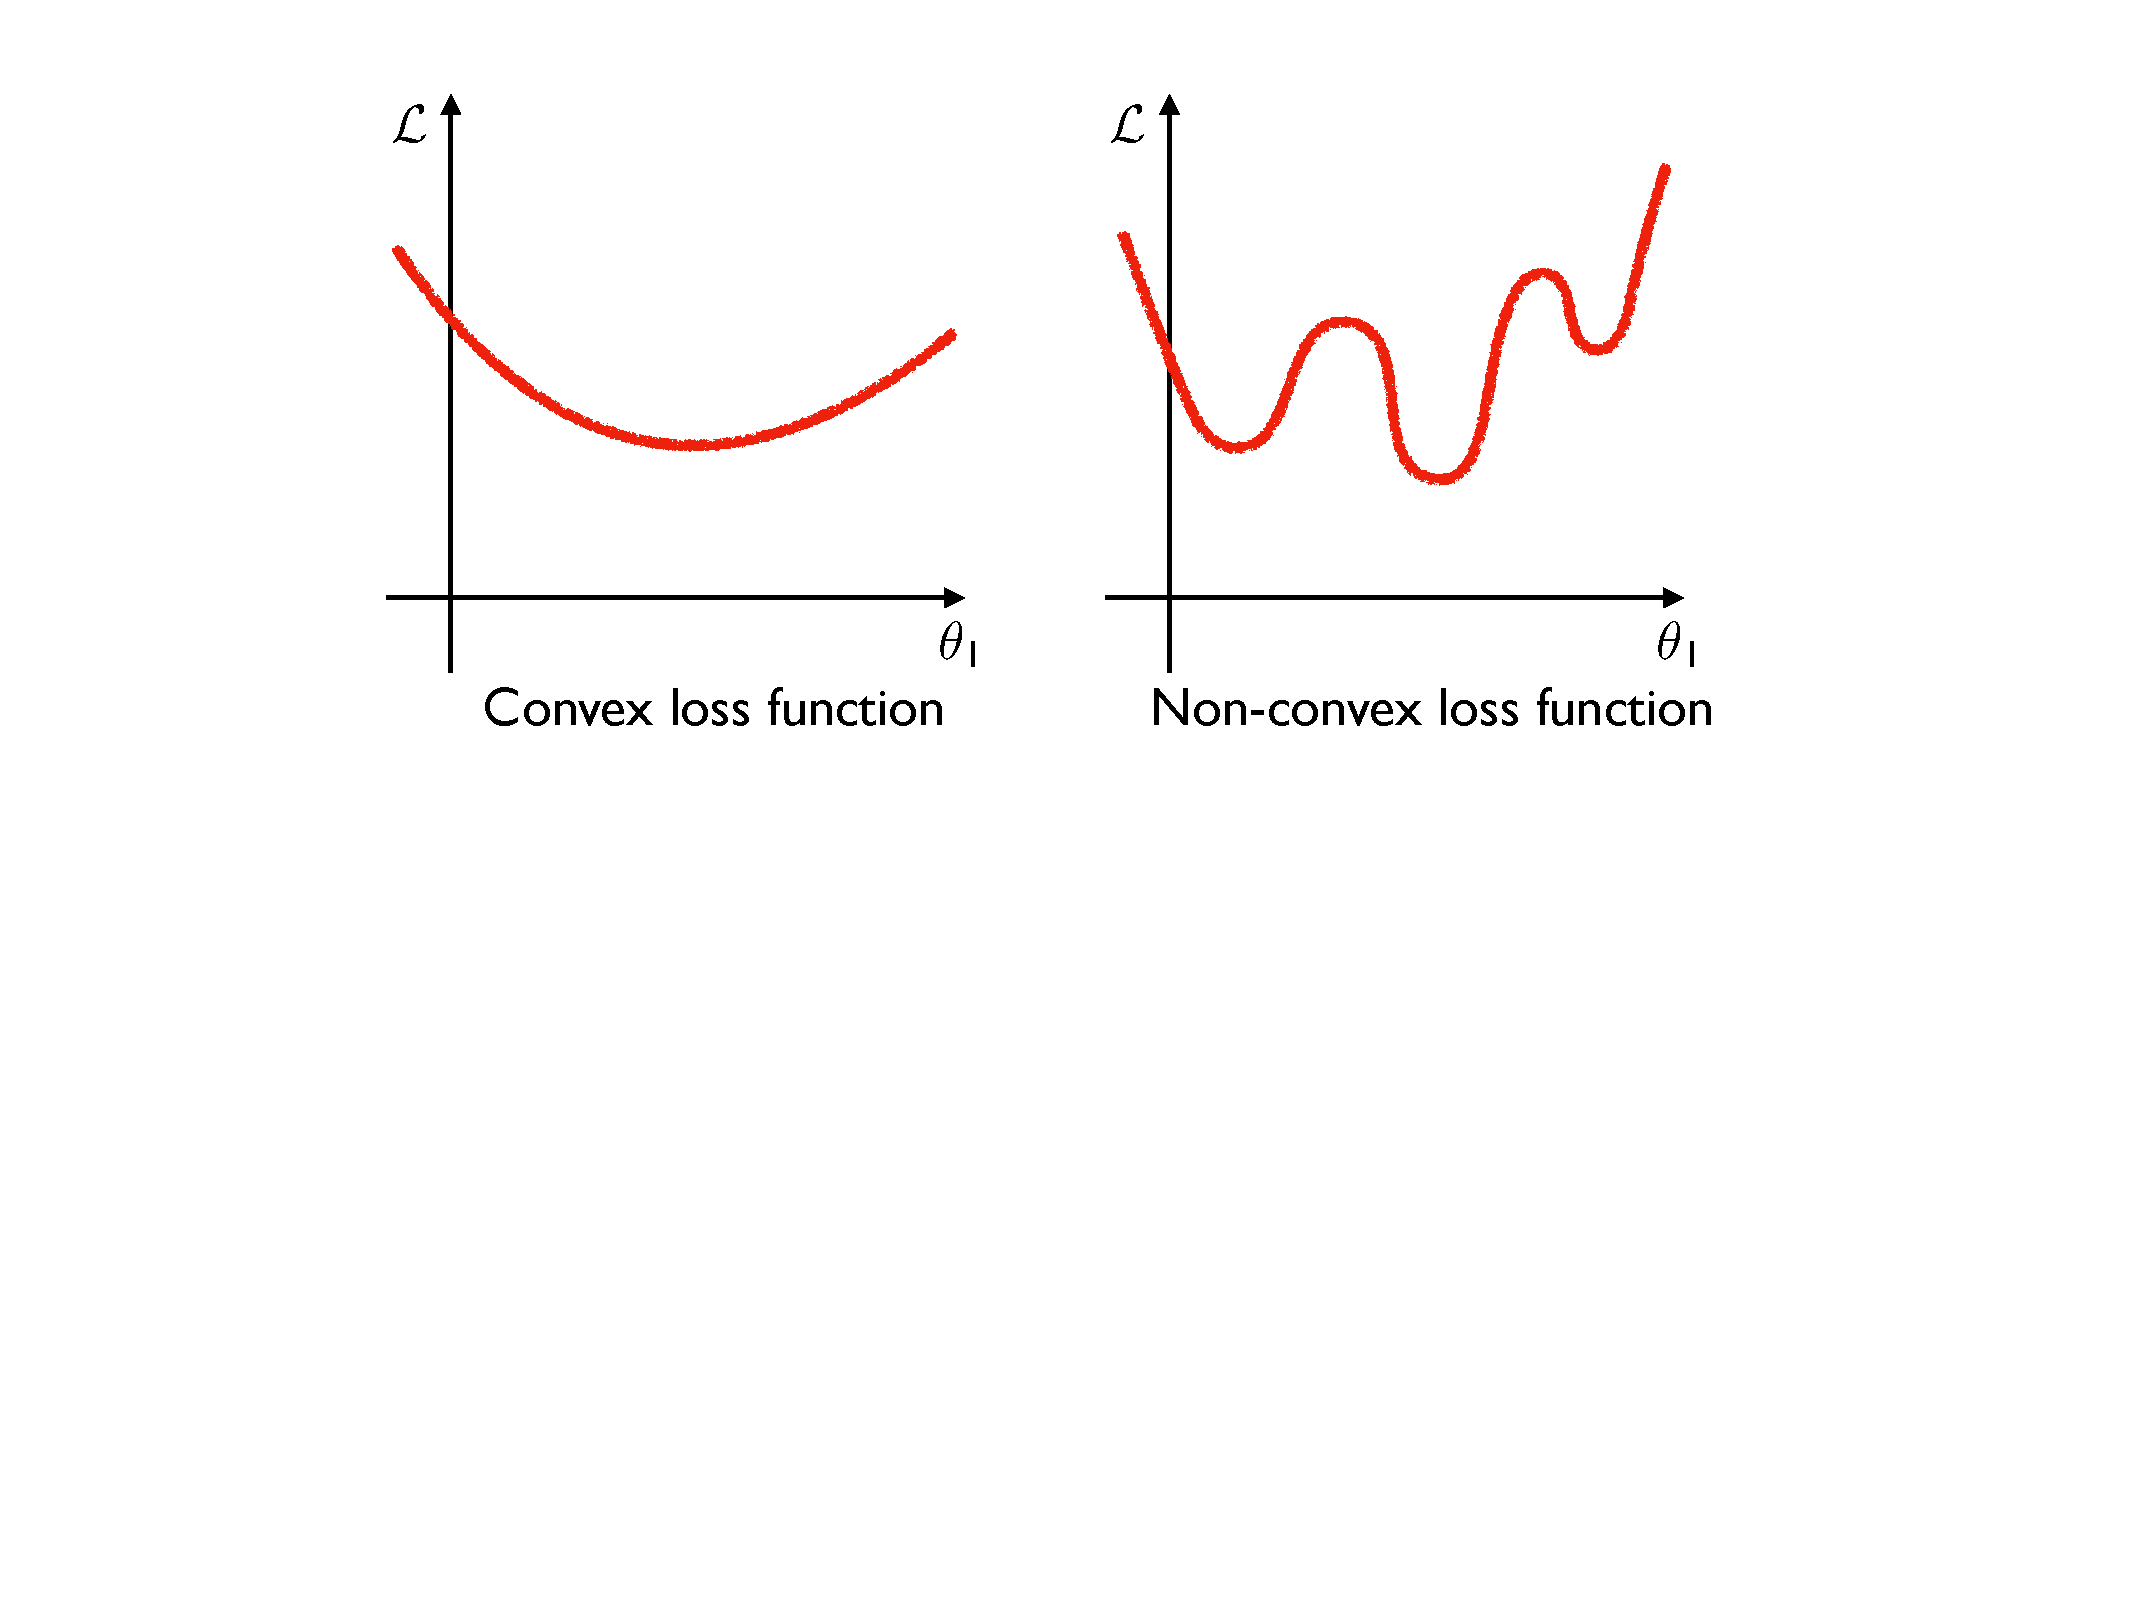
\includegraphics[width=0.9\textwidth]{../graphics/Vis_convexity.pdf}
\end{figure}
\begin{itemize}
	\item Convex optimization functions: only one local minimum (which is also the global minimum). 
	\item In neural networks, the loss is often not convex. 
	\item The shape of the loss is very important for the success of the optimization. 
	\item How can we visualize the loss w.r.t $\sim10^6$ parameters? 
\end{itemize}
\end{frame}

\begin{frame}{Visualization of the loss function}
\begin{itemize}
	\item Visualizations are limited to 2D or 3D plots.
	\item We can only plot the loss as a function of one or two parameters. 
	\item Idea: to draw two {\bf random directions} $\delta$, $\eta$ in parameter space and plot the loss function in these directions:
	\begin{equation}
	\loss (\alpha, \beta) = L(\param^{\ast} + \alpha \delta + \beta \eta) 
	\end{equation}
	with $\param^{\ast}$ our solution which is supposed to be optimal. 
	\item Alternative: if we wish to compare two networks $\param^A$ and $\param^B$, we can also visualize the loss in the direction of the difference between these two points in parameter space \cite{Goodfellow:2015}:
	\begin{equation}
		\param(\alpha) = (1 - \alpha)\param^A + \alpha \param^B
	\end{equation}
\end{itemize}
\end{frame}

\begin{frame}{The sharpness of a minimum}
\begin{figure}[htb]
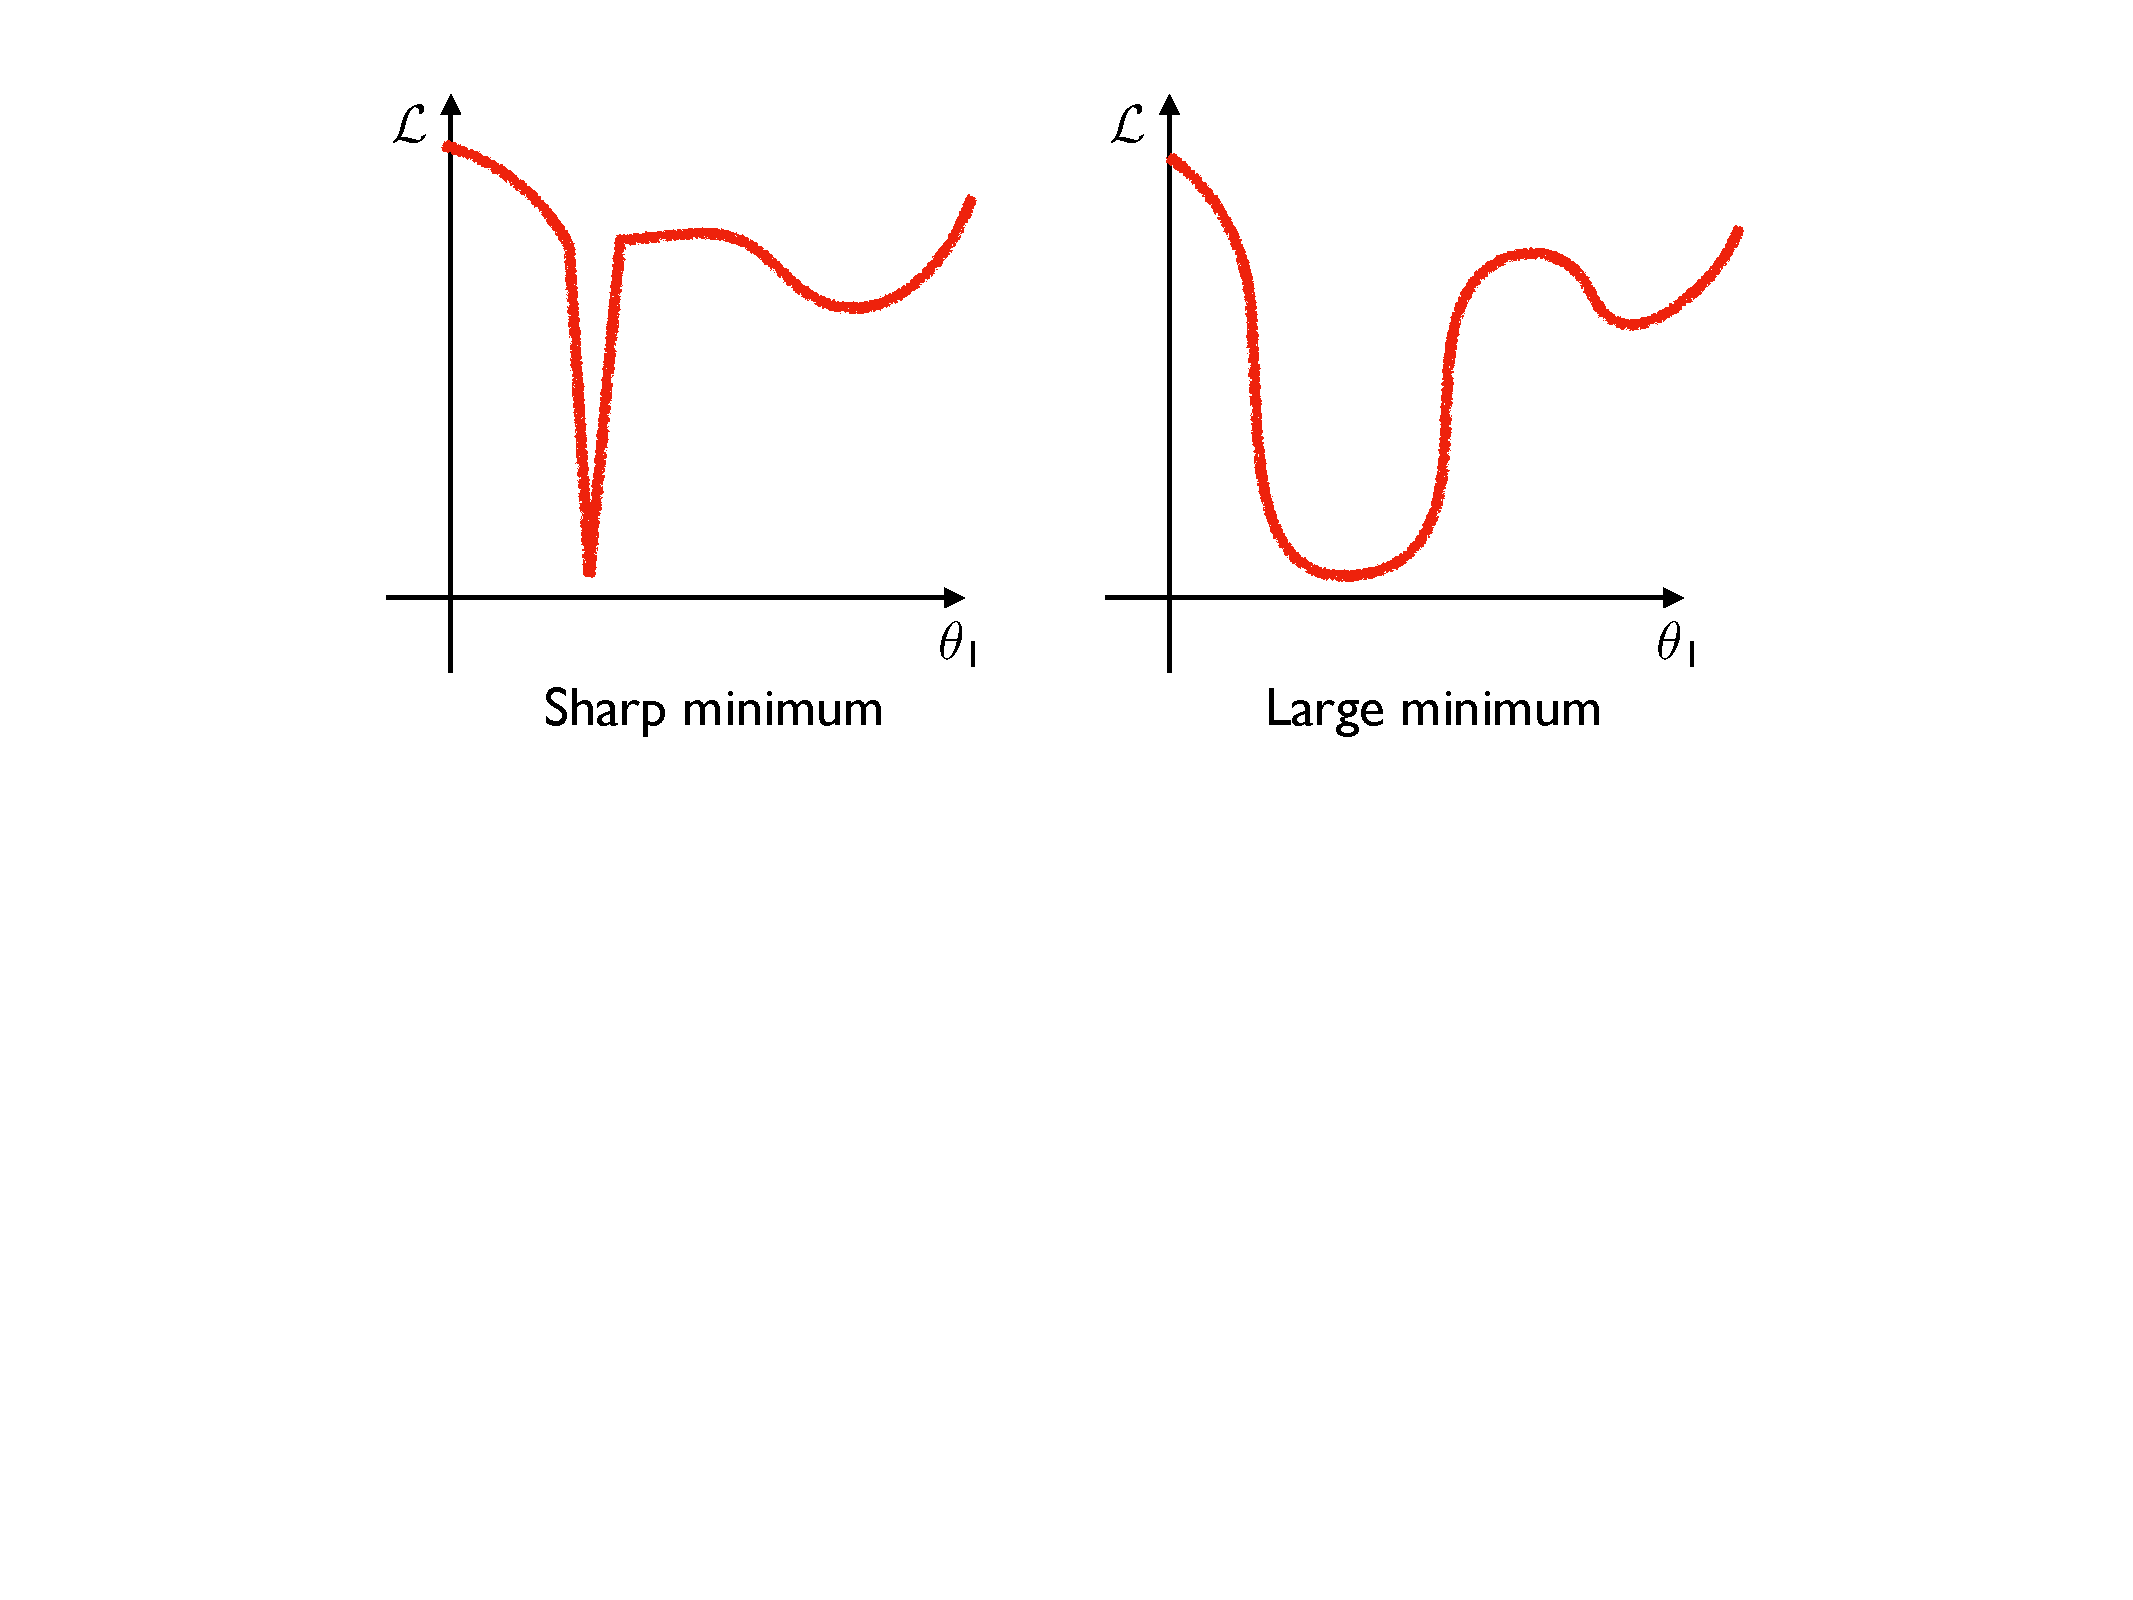
\includegraphics[width=0.9\textwidth]{../graphics/Vis_sharpness.pdf}
\end{figure}
\begin{itemize}
	\item Sharpness of a minimum: the intuition is that sharp minima are hard to find and less robust. 
	\item Can we use visualization in order to assess the sharpness of a minimum? 
\end{itemize}
\end{frame}

\begin{frame}{Scale invariance and filter-wise normalization}
\begin{itemize}
	\item Scale invariance: two neural networks with ReLu as non-linearities are equivalent, if we multiply the weights of one layer with a factor and divide the weights of the next layer by the same factor. 
	\item 1D and 2D plots of the loss can therefore be misleading: the sharpness of a minimum might be due to a large extent to the problem of scale invariance. 
	\item One idea to cope with scale invariance is to normalize the directions with respect to the filter weights \cite{Li:2018}:
	\begin{itemize}
		\item First we draw a random direction $d$ (same dimension as $\param$). 
		\item For visualization, we require that the values in $d$ that correspond to filter $j$ in layer $i$ have the same norm as the parameter values $(i,j)$:
%		directional values in $d$ corresponding to filter parameters $(r,l)$ have the same norm as the filter values. 
		\begin{equation}
			d_{i,j} \leftarrow \frac{d_{i,j}}{\|d_{i,j}\|}\|\param_{i,j}\|
		\end{equation}
		where $\|\cdot\|$ is the Frobenius norm. This filter-wise normalization ensures that we can interpret the produced maps.
	\end{itemize}
\end{itemize}
\end{frame}

\begin{frame}{Example: effect of deeper networks}
\begin{figure}[htb]
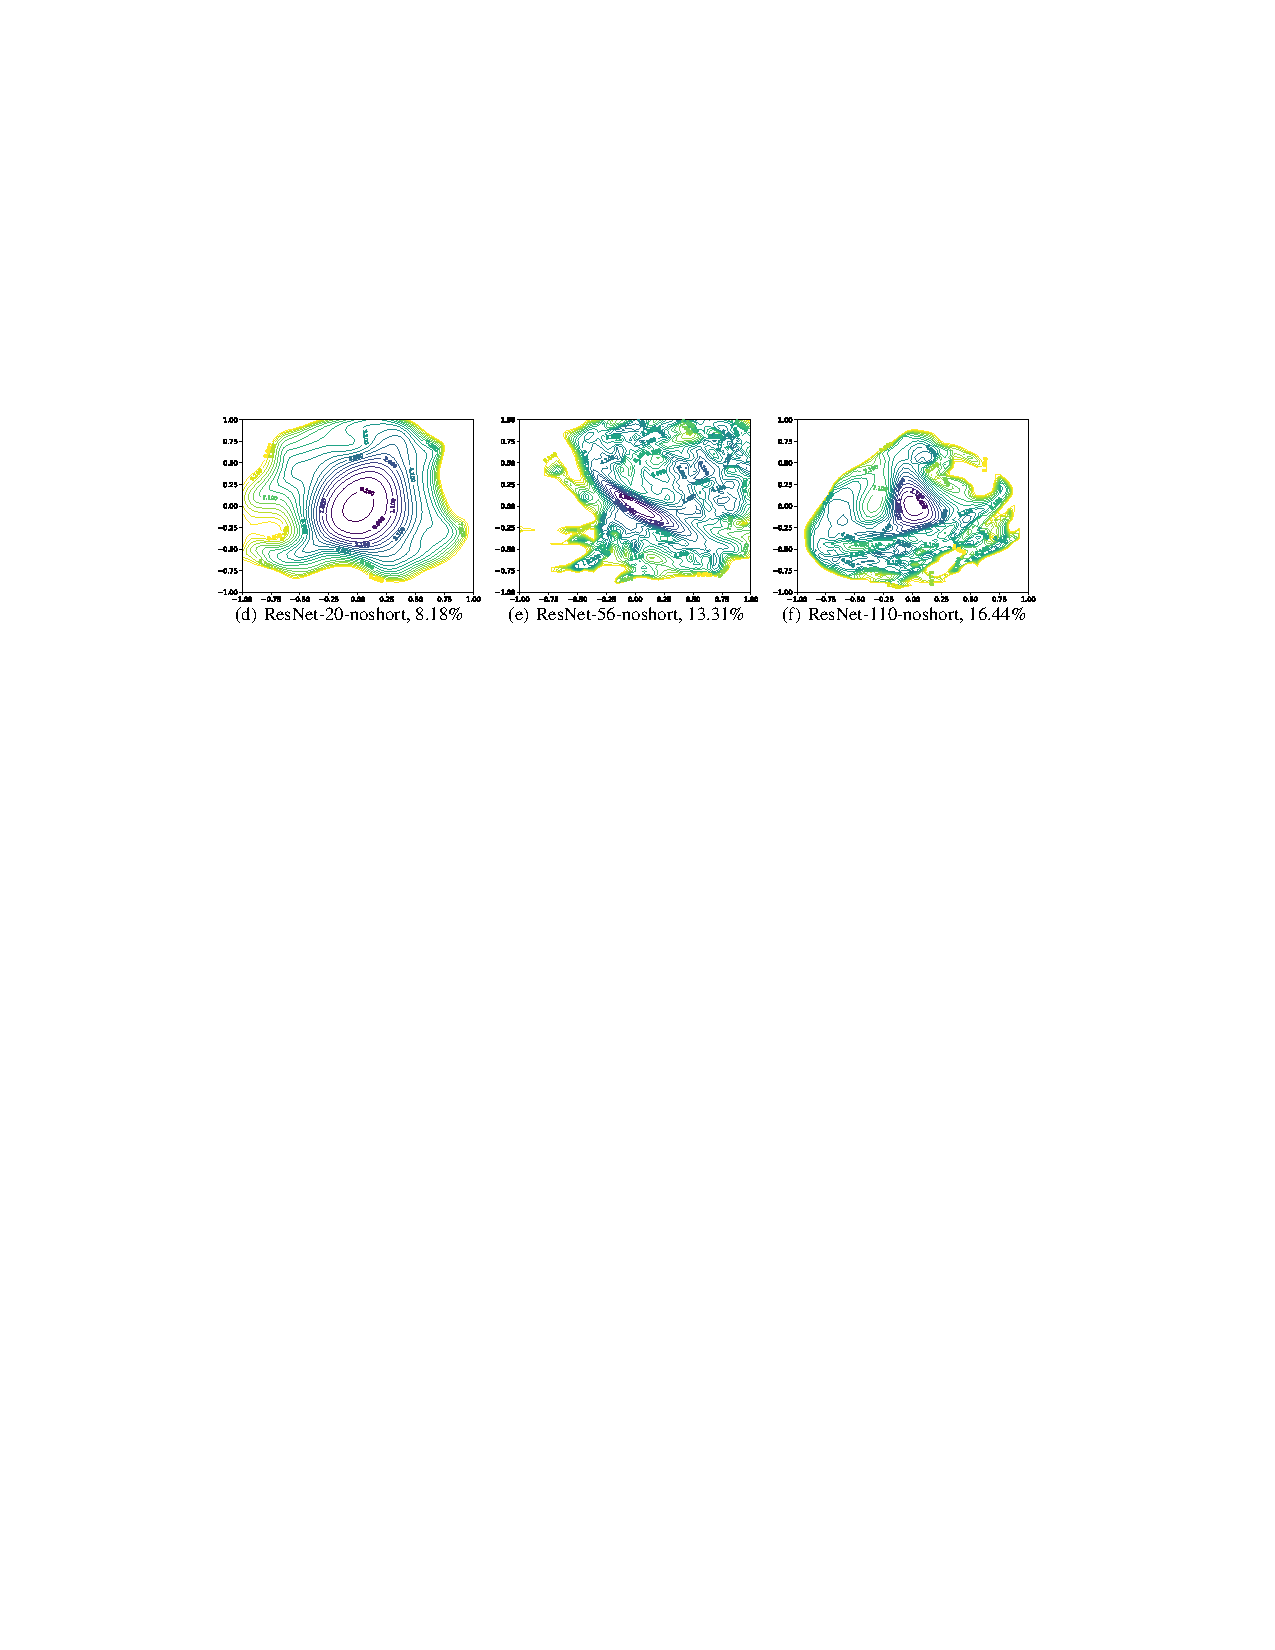
\includegraphics[width=0.9\textwidth]{../graphics/Vis_resnet_without_skip_2d.pdf}
\caption{Resnet architecture without skip connections (varying depth)}
\source{From \cite{Li:2018}}
\end{figure}
\begin{itemize}
	\item With 20 layers, we observe a fairly convex loss function. 
	\item With more layers, the loss function becomes chaotic and the gradient does not point to the global minimum. 
	\item In addition, the minima are steep and sometimes ill-conditioned (anisotropy). 
\end{itemize}
\end{frame}

\begin{frame}{Example: importance of skip-layers}
\begin{figure}[htb]
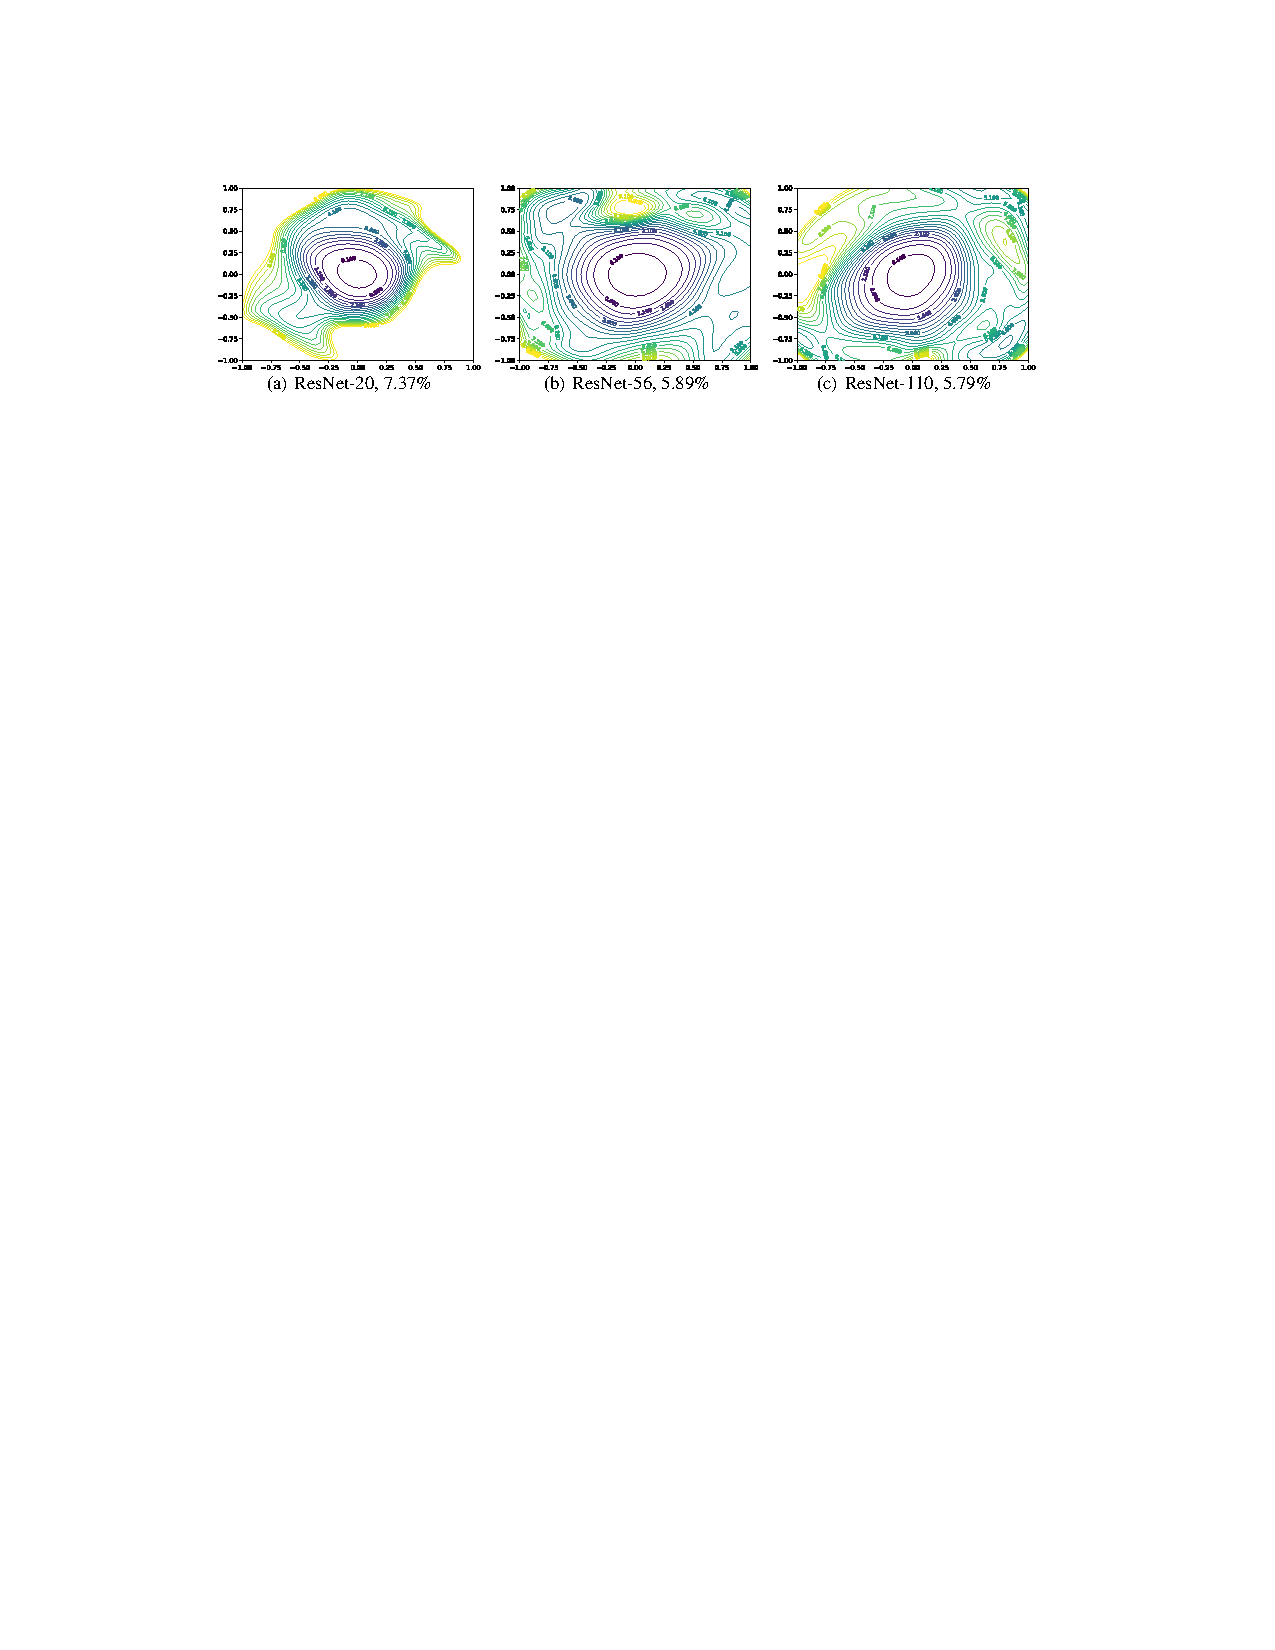
\includegraphics[width=0.9\textwidth]{../graphics/Vis_resnet_with_skip_2d.pdf}
\caption{Resnet architecture with skip connections (varying depth)}
\source{From \cite{Li:2018}}
\end{figure}
\begin{itemize}
\item Adding skip connections makes the objective function "more convex". 
\item This is particularly true for deeper networks (here: 56 and 110 layers). 
\item We therefore understand the impact of this architectural choice.
\end{itemize}
\end{frame}

\begin{frame}{More examples for the importance of skip-layers}
\begin{figure}[htb]
  \centering
  \subfloat{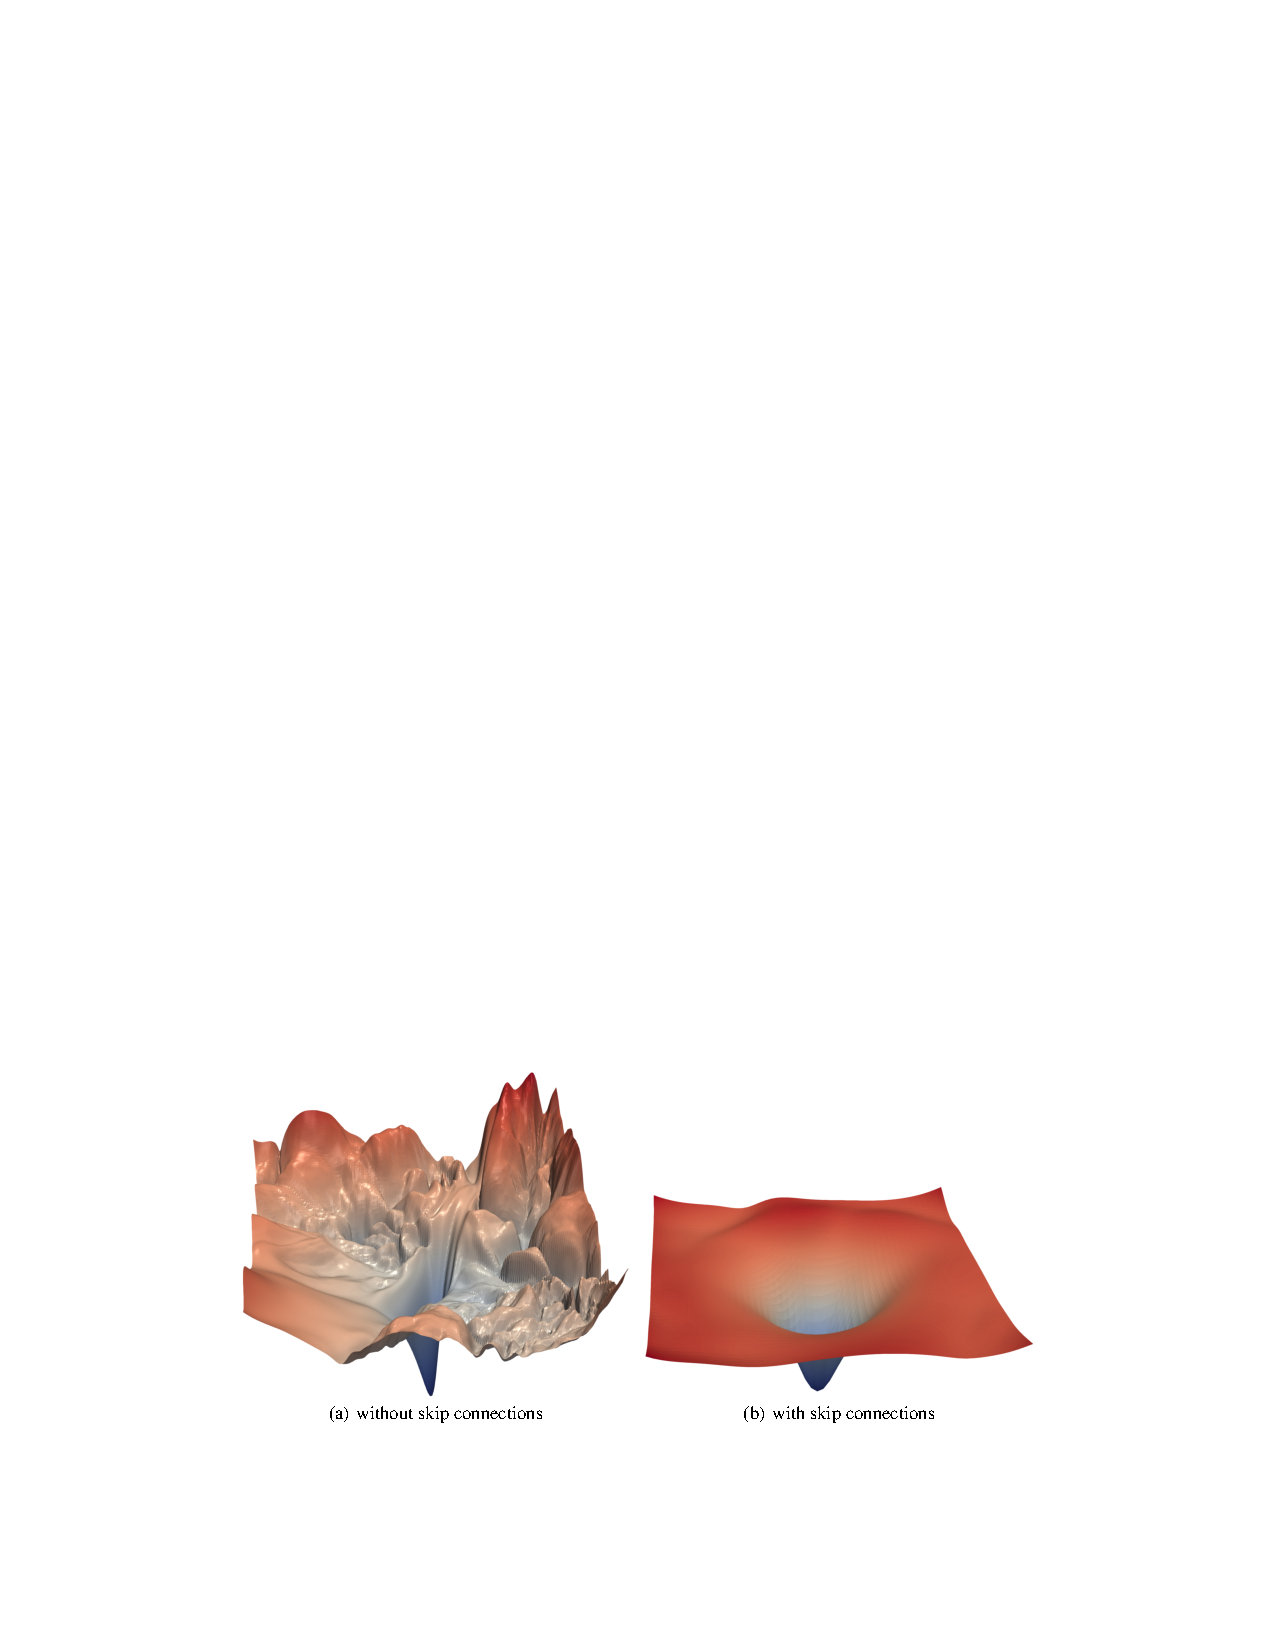
\includegraphics[width=0.7\textwidth]{../graphics/Vis_resnet_comparison_3d.pdf}}\\
  \subfloat{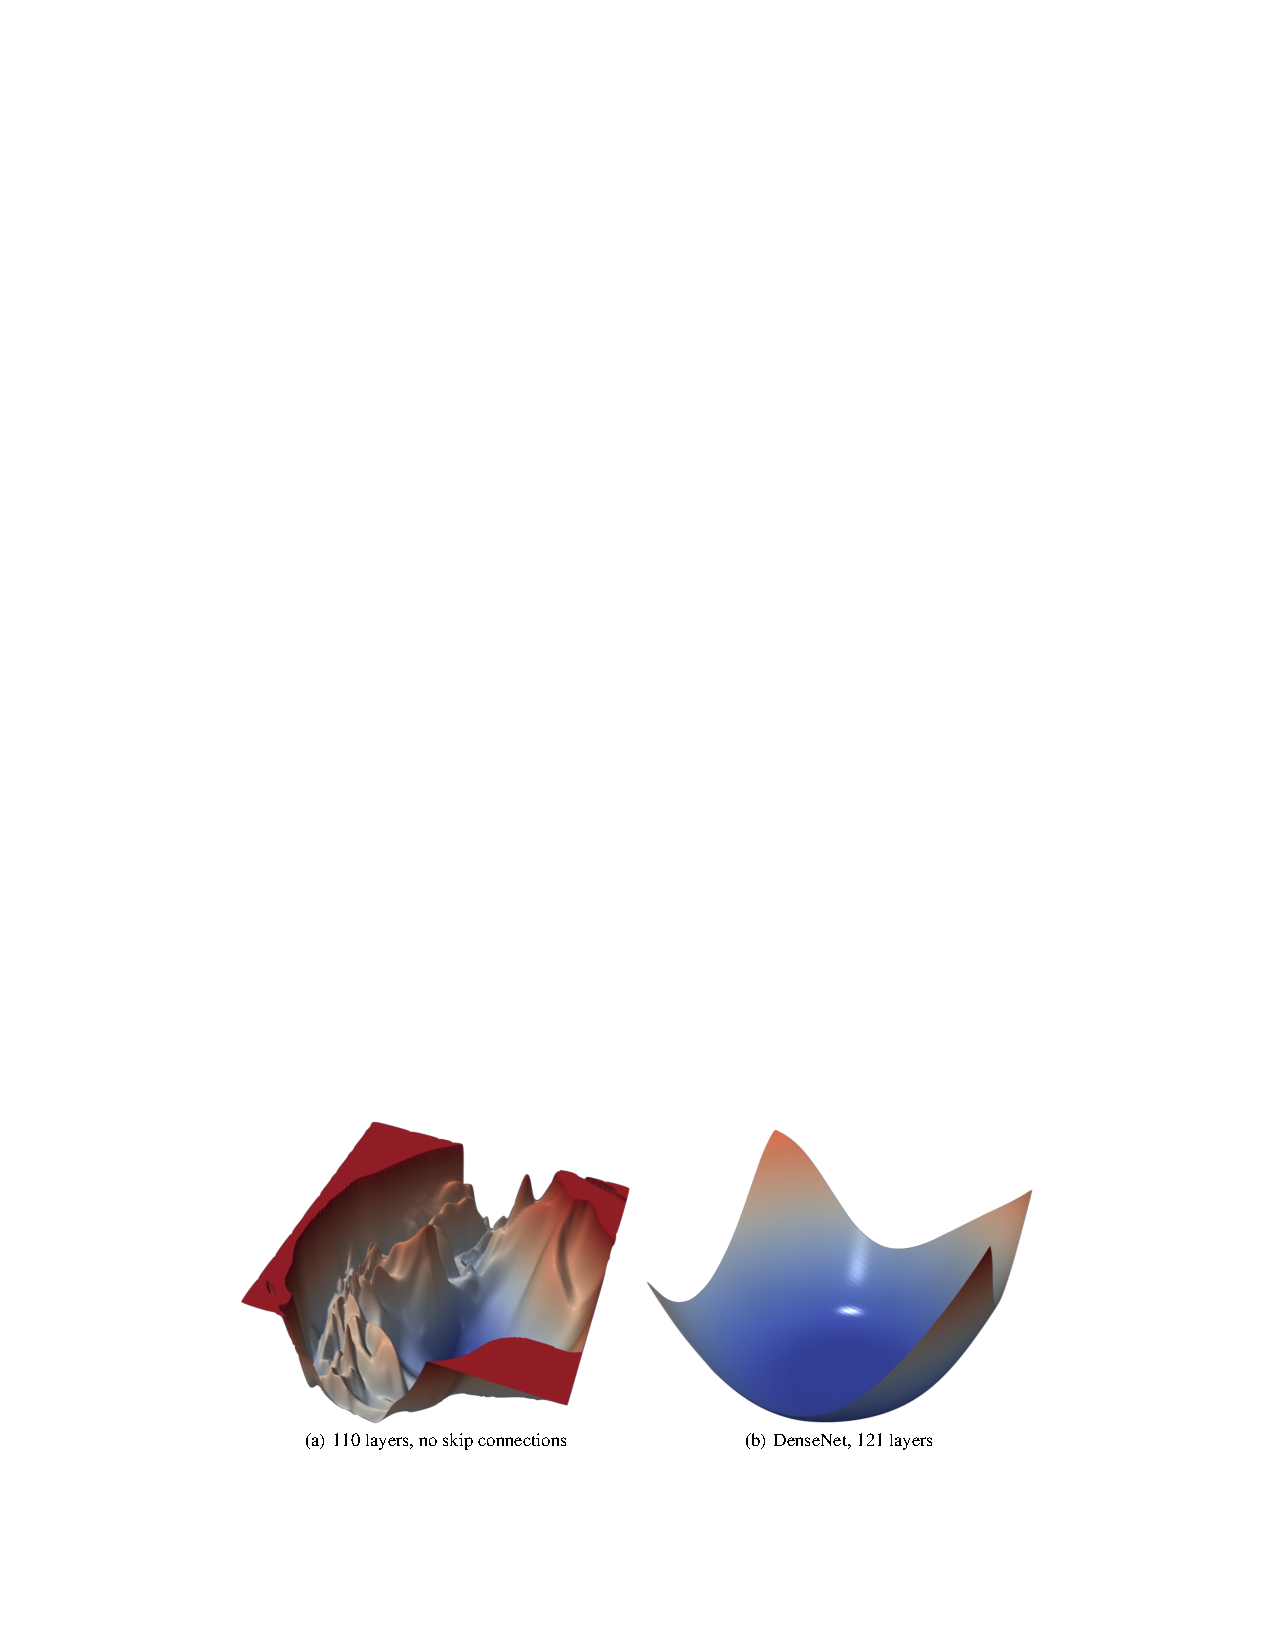
\includegraphics[width=0.7\textwidth]{../graphics/Vis_resnet_comparison2_3d.pdf}} 
  \source{From \cite{Li:2018}}
\end{figure}
\end{frame}

\section{Conclusion}
\frame{\frametitle{Overview}\tableofcontents[currentsection]}

\begin{frame}{What lessons do we learn?}
	\begin{itemize}
		\item Features are extracted hierarchically. 
		\item The first layer typically extracts low-level color and contour features.
		\item Later layers extract more specialized features (combinations of low-level features). This is the reason why you normally extract more feature maps in higher layers.
		\item We have methods to investigate the image regions that are responsible for classification assignments, and we can therefore understand, on which grounds a decision is made.
		\item Visualization of the loss function allows to compare architectures and to study architectural choices. 
		\item As an example, skip layers "convexify" the loss function.
	\end{itemize}
\end{frame}

%%%%%%%%%%%%%%%%%%%%%%%%%%%%%%%%%%%%%%%%%%%%%%%%%%%%%%%%%%%%%%%%%%%%%%%%%
%%%%%%%%%%%%%%%%%%%%%%%%%%%%%%%%%%%%%%%%%%%%%%%%%%%%%%%%%%%%%%%%%%%%%%%%%
\section{References}
\begin{frame}[allowframebreaks]
	\frametitle{References}
	\bibliography{slides_deep.bib}
\end{frame}


\end{document}